\documentclass[10pt,oneside]{book}
\usepackage[T1]{fontenc}
\usepackage{lmodern}
\usepackage{yfd,symbols}
\usepackage{xcolor}
\usepackage{fancyhdr}
\usepackage[normalem]{ulem}
\pagestyle{fancy}
\fancyhead{}
\fancyfoot{}

\fancyhead[C]{\normalsize\bf\sffamily Page:~\thepage}
\fancyhead[R]{\bfseries \rightmark}
\fancyhead[L]{\bfseries \leftmark}
\renewcommand{\chaptermark}[1]{\markboth{#1}{}}
\renewcommand{\sectionmark}[1]{\markright{#1}}
\renewcommand{\headrulewidth}{1pt}
\setcounter{secnumdepth}{3}
\setcounter{tocdepth}{2}

\usepackage[
    backend=biber,
    style=authoryear,
    natbib=true,
    giveninits=true,
    uniquename=init,
    maxbibnames=10,
    minbibnames=10,
    maxcitenames=2,
    mincitenames=1
]{biblatex}
\addbibresource{ref.bib}
\DeclareDelimFormat{nameyeardelim}{\addcomma\space}
\DeclareDelimFormat{multicitedelim}{\addsemicolon\space}
\DeclareDelimFormat{compcitedelim}{\addsemicolon\space}


\begin{document}
\frontmatter
\hypersetup{linkcolor=black}
\begin{titlepage}
\centering
\vspace*{6cm}
{\Huge\bf\sffamily Post-Training HandBook\par}
\vspace{1.5cm}
{\large\sffamily Last Update: \today\par}
\vfill
\end{titlepage}
\tableofcontents
\hypersetup{linkcolor=softblue}

\mainmatter
\chapter{Introduction}
\section{Background Knowledge}

\subsection{Markov Decision Process}
\begin{definition}[State, Action, Trajectory]
A sequence of actions and states with $T$ interactions with environment is defined as a trajectory $\tau = (s_0, a_0, s_1,a_1,s_2,a_2,\ldots, a_{T-1}, s_{T-1})$ 
\end{definition}

\begin{definition}[Reward and Return] 
% A single step reward $r_t$ is determined by the current state $s_t$ the action taken $a_t$ and the state $s_{t+1}$ after the action $a_{t}$ is taken. It is defined as $r_t := R(s_t,a_t,s_{t+1})$. 
At time step $t$, the agent observes state $s_t$, takes action $a_t$, and transitions to the next state $s_{t+1}$. The single-step reward is determined by the transition and is defined as
$$
r_t = R(s_t,a_t,s_{t+1}).
$$ 
The (discounted) \textbf{reward} on the trajectory $\tau$ is defined as 
$$
    R(\tau) = \sum_{t=0}^{t-1}\gamma^{t}r_t,
$$
where $\gamma\in(0,1]$ is the discount factor. The discounted \textbf{return} starting from time step $t$ is defined as
$$
    G_t(\tau) = \sum_{t'=t}^{T-1}\gamma^{t'-t}r_{t'}. 
$$
Equivalently, $G_t$ satisfies the recursive relation
$$
G_t = r_t + \gamma G_{t+1}.
$$
\end{definition}


\begin{definition}[State-Value Function and Value Function]
The value function for the policy $\pi$ is defined as
$$
% V^{\pi}(s_t) = \Embb_{\pi} [G_t | s_t] = \Embb_{a_t\sim \pi(.|s_t)}\Embb_{s_{t+1}\sim P(.|s_t, a_t)}\left[r_t + \gamma V^{\pi}(s_{t+1})\right].
\begin{aligned}
V^\pi(s_t)
&= \Embb_{\pi} [G_t \mid s_t]  = \Embb_{\pi} [r_t + \gamma G_{t+1} \mid s_t] = \mathbb{E}_{a_t\sim \pi(\cdot\mid s_t)}
\mathbb{E}_{s_{t+1}\sim P(\cdot\mid s_t,a_t)}
\left[
r_t + \gamma \Embb_{\pi}[G_{t+1}\mid s_{t+1}]
\right] \\
&= \mathbb{E}_{a_t\sim \pi(\cdot\mid s_t)}
\mathbb{E}_{s_{t+1}\sim P(\cdot\mid s_t,a_t)}
\left[
r_t + \gamma V^\pi(s_{t+1})
\right].
\end{aligned}
$$

The state-value function for the policy $\pi$ is defined as
$$
Q^{\pi}(s_t, a_t) = \Embb_{\pi} [G_t | s_t, a_t] = \Embb_{s_{t+1}\sim P(.|s_t, a_t)}\left[r_t + \gamma V^{\pi}(s_{t+1})\right].
$$
Therefore,
$$
V^{\pi}(s_t) = \Embb_{a_t\sim \pi(.|s_t)} [Q^{\pi}(s_t, a_t)]
$$
\end{definition}



\begin{definition}[Advantage]
The advantage function, by it’s definition, measures whether or not the action is better or worse than the policy’s default behavior.
    \begin{align}
        A^{\pi}(s_t, a_t) 
        & =  Q^{\pi}(s_t, a_t) - V^{\pi}(s_t)  = \Embb_{s_{t+1}\sim P(.|s_t, a_t)} \left[\underbrace{r_t + \gamma V^{\pi}(s_{t+1}) -  V^{\pi}(s_t)}_{\text{temporal difference}}\right]
    \end{align}
    
\end{definition}

\subsection{Useful Facts}

\begin{enumerate}
    \item  Probability of a trajectory 
        \begin{align}
        P(\tau | \theta)=\rho_0\left(s_0\right) \prod_{t=0}^{T-1} P\left(s_{t+1} | s_t, a_t\right) \pi_\theta\left(a_t | s_t\right) \label{eq:prob.of.a.trajectory}
        \end{align}
     \item  log derivative trick
         \begin{align}
        \grad_{\theta} P(\tau | \theta)=  P(\tau | \theta) \grad_\theta \log P(\tau | \theta)\label{eq:log.derivative.trick}
        \end{align}
    \item expected Grad-Log-Prob Lemma
        \begin{align}\label{eq:grad.log.prob}
            \Embb_{x\sim p(\cdot;\theta)} [\grad_{\theta} \log p(x;\theta)] = 0
        \end{align}

    
\end{enumerate}


\subsection{Glossaries}
\begin{definition}[Estimation of the $\operatorname{KL}$ divergence]\label{def:kl-est}
    There are different estimators of the KL divergence, which can be found \href{http://joschu.net/blog/kl-approx.html}{here}. Recall that $\operatorname{KL}(q||p)=E_{x\sim q}\left[\log \frac{q(x)}{p(x)}\right]$,
    
    \begin{itemize}
        \item $k_1$ estimator: $\frac{1}{n}\sum_{i=1}^{n} \log \frac{q(x_i)}{p(x_i)}$. Unbiased, high variance. Can be negative.
        \item $k_2$ estimator:  $\frac{1}{n}\sum_{i=1}^{n} \frac{1}{2}\left(\log \frac{p(x_i)}{q(x_i)}\right)^2$. biased, low variance. Always positive.
        \item  $k_3$ estimator: $\frac{p(x)}{q(x)} - 1 - \log \frac{p(x)}{q(x)}$. Always positive. Better than $k_2$? (non-negativity: $\log a \leq a - 1$ for all $a>0$).
    \end{itemize}
\end{definition}

\yd{To add: comparison with three estimators}
\section{Policy Gradient}

The goal of the policy-based RL is to maximize the expected reward 

\begin{align}
    \max \left\{\Jcal(\theta):= \Embb_{\tau\sim \pi_{\theta}}\left[ R(\tau)\right] = \int P(\tau|\theta)R(\tau) d\tau\right\},
\end{align}
where $P(\tau|\theta)$ is defined in \eqref{eq:prob.of.a.trajectory} and $s_0\sim \rho_0(\cdot)$
\begin{itemize}
    \item $a_t\sim \pi_{\theta}(\cdot | s_t)$ for all $t\in \{0, 1, \ldots, T-1\}$.
    \item $s_{t+1} \sim P(\cdot | s_t, a_t)$ for all $t\in \{0, 1, \ldots, T-1\}$.
    \item $r_t=R(s_t,a_t, s_{t+1})$ for all $t\in \{0, 1, \ldots, T-1\}$.
\end{itemize}

Applying \eqref{eq:prob.of.a.trajectory} and \eqref{eq:log.derivative.trick}, we get 
\begin{align}
    \grad_{\theta} \Jcal(\theta) 
    & = \int \grad_{\theta} P(\tau|\theta)R(\tau) d\tau = \int  P(\tau|\theta) \grad_{\theta}\log  P(\tau|\theta)R(\tau) d\tau = \Embb_{\tau\sim \pi_{\theta}}\left[ \grad_{\theta}\log P(\tau|\theta)R(\tau)\right] \nonumber\\
    & = \Embb_{\tau\sim \pi_{\theta}}\left[ \grad_{\theta}\left(\rho_0\left(s_0\right) + \sum_{t=0}^{T-1} P\left(s_{t+1} | s_t, a_t\right)\right) + \sum_{t=0}^{T-1}\grad_{\theta} \log \pi_\theta\left(a_t | s_t\right)\right] R(\tau) \nonumber\\
    & = \Embb_{\tau\sim \pi_{\theta}}\left[ R(\tau) \sum_{t=0}^{T-1}\grad_{\theta} \log \pi_\theta\left(a_t | s_t\right)\right] \label{eq:policy.grad}
\end{align}



\subsection{Policy Gradient Estimator}

Given $N$ trajectories $\{\tau_1, \ldots, \tau_N\}$ with $\tau_n\sim \pi_{\theta}$ for all $n\in [N]$, how can we construct a "good" policy gradient estimator?

The natural choice would be
\begin{itemize}
    \item Naive unbiased estimator
    $$
    \widetilde{\grad_{\theta} \Jcal(\theta)}  = \frac{1}{N}\sum_{n=1}^{N} \left(  \sum_{t=0}^{T_{n}-1} R(\tau_n) \grad_{\theta} \log \pi_\theta\left(a_t | s_t\right) \right)
    $$
\end{itemize}
However, the above looks a bit weird in the sense that $\log \pi_\theta\left(a_t | s_t\right)$ contains single-step probability while $R(\tau_n)$ represents the whole trajectory. This naturally leads to the following abstraction
 $$
    \widetilde{\grad_{\theta} \Jcal(\theta)}  = \frac{1}{N}\sum_{n=1}^{N} \left(  \sum_{t=0}^{T_{n}-1} \Phi_t \grad_{\theta} \log \pi_\theta\left(a_t | s_t\right) \right)
$$
Some popular choices of $\Phi_t$\citep{schulman2015high}, hence the gradient estimator can be
\begin{itemize}
    \item Reward-to-go unbiased estimator (drops $a_t$'s dependency on the past actions)
    $$
    \widetilde{\grad_{\theta} \Jcal(\theta)}  = \frac{1}{N}\sum_{n=1}^{N} \left(\sum_{t=0}^{T_{n}-1}G_t(\tau_n)\grad_{\theta}\log \pi_\theta\left(a_t | s_t\right) \right)
    $$
    Recall $G_t(\tau) = \sum_{t'=t}^{T-1}\gamma^{t'-t}r_t'$. If one adopts this estimator, then the algorithm is called \textbf{REINFORCE} algorithm. This method drops the need on the Value function (see details below) but suffers from the high variance in gradient estimates.
    \item with baseline (variance reduction)
    $$
    \widetilde{\grad_{\theta} \Jcal(\theta)}  = \frac{1}{N}\sum_{n=1}^{N} \left(  \sum_{t=0}^{T_{n}-1} (G_t(\tau_n) - b(s_t)) \grad_{\theta} \log \pi_\theta\left(a_t | s_t\right) \right)
    $$
    One popular choice of the baseline function is $b(s_t):=V^{\pi}(s_t)$. When $V^{\pi}$ is unknown, we can approximate it with $V^{\pi}_{\phi}(\cdot)$, a neural network parameterized by $\phi$.

    \item Advantages based estimator 
     $$
    \widetilde{\grad_{\theta} \Jcal(\theta)}  = \frac{1}{N}\sum_{n=1}^{N} \left(\sum_{t=0}^{T_{n}-1}A^{\pi}(s_t, a_t) \grad_{\theta} \log \pi_\theta\left(a_t | s_t\right) \right),
    $$
    where $A^{\pi}(s_t, a_t)=Q^{\pi}(s_t, a_t) - V^{\pi}(a_t)$.

    \item TD-error based estimator 
     $$
    \widetilde{\grad_{\theta} \Jcal(\theta)}  = \frac{1}{N}\sum_{n=1}^{N} \left( (r_t+\gamma V^{\pi}(s_{t+1}) - V^{\pi}(s_t)) \sum_{t=0}^{T_{n}-1}\grad_{\theta} \log \pi_\theta\left(a_t | s_t\right) \right),
    $$
    where $r_t+\gamma V^{\pi}(s_{t+1}) - V^{\pi}(s_t)$ is a approximation of the $A^{\pi}(s_t, a_t)$.

    \item GAE$(\gamma, \lambda)$ estimator
    $$
    \widetilde{\grad_{\theta} \Jcal(\theta)}  = \frac{1}{N}\sum_{n=1}^{N} \left( \sum_{\ell=0}^{T_n}(\gamma\lambda)^{\ell}\delta_{t+\ell} \sum_{t=0}^{T_{n}-1}\grad_{\theta} \log \pi_\theta\left(a_t | s_t\right) \right),
    $$
    where $\delta_t=r_t + \gamma V^{\pi}_{\phi}(s_{t+1}) -  V^{\pi}_{\phi}(s_{t})$.
    GAE$(\gamma, 0)$ typically has low variance and GAE$(\gamma, 1)$ has high variance.
\end{itemize}

\subsection{REINFORCE algorithm}
If one adopts the Reward-to-go unbiased estimator, we can reach to the REINFORCE algorithm. The objective function is
\begin{equation}
\label{eq:reinforce.obj}
     \Jcal(\theta)  = \Embb_{\tau\sim \pi_\theta}\left(\sum_{t=0}^{T-1}G_t(\tau)\log \pi_\theta\left(a_t | s_t\right) \right)
\end{equation}
where $G_t(\tau) = \sum_{t'=t}^{T-1}\gamma^{t'-t}r_{t'}$. 
This method drops the need on the Value function but suffers from the high variance in gradient estimates. The algorithm is summarized in Algorithm~\ref{algo:reinforce}

\begin{algorithm}[H]
\caption{REINFORCE}
\begin{algorithmic}[1]
    \State Inputs: Initial Policy network parameter $\theta_0$ and stepsize $\alpha$.
    \For{k=0,1,2....}
        \State Collect a set of trajectories $D_k=\{\tau_n\}_{n=1}^{N}$.
        \State Reward-to-go calculation $G_t(\tau_n) = \sum_{t'=t}^{T_n-1}\gamma^{t'-t}r_t'$ for all $n$.
        \State Compute the gradient estimate
         $$
            \widetilde{\grad_{\theta} \Jcal(\theta_k)}  = \frac{1}{N}\sum_{n=1}^{N} \left(\sum_{t=0}^{T_{n}-1}G_t(\tau_n)\grad_{\theta}\log \pi_{\theta_k}\left(a_t | s_t\right) \right)
        $$
        \State Policy update $\theta_{k+1} \gets \theta_k + \alpha \widetilde{\grad_{\theta} \Jcal(\theta_k)}$
    \EndFor
\end{algorithmic}
\label{algo:reinforce}
\end{algorithm}


\subsection{Actor-Critic Algorithm} 
When one adopts the estimator for the policy gradient, usually the state value function is used. Let us approximate it with $V^{\pi}_{\phi}$ the objective function for TD-residual based gradient estimator can written as

\begin{align*}
     \max \left\{\Jcal_{\text{TD}}(\theta):= \Embb_{\tau\sim \pi_{\theta}}\left[ \sum_{t=0}^{T-1}(r_t+\gamma V^{\pi}_{\phi}(s_{t+1}) - V^{\pi}_{\phi}(s_{t}))\log\pi_{\theta}(a_t|s_t)\right]\right\}.
\end{align*}

Similarly, the $V^{\pi}_{\phi}$ can be updated by

\begin{align}
     \min \left\{\Lcal(\phi):= \Embb_{\tau\sim \pi_{\theta}}\left[ \sum_{t=0}^{T-1}[(r_t+\gamma V^{\pi}_{\phi}(s_{t+1}) - V^{\pi}_{\phi}(s_t)]^2\right]\right\}.
     \label{eq:naive.critic.obj}
\end{align}

This is actually the actor-critic framework. When we drive $\Lcal(\phi)$ to 0, intuitively, the advantage will be close to 0, which means that for the actor, $\pi_{\theta}$ is approaching the optimal policy and the value function is also approaching the optimal.


\yd{To add}

\begin{algorithm}[H]
\caption{Naive Actor-Critic Algorithm}
\begin{algorithmic}[1]
    \State Inputs: Initial Policy network parameter $\theta_0$ and stepsize $\alpha$.
    \For{k=0,1,2....}
        \State Collect a set of trajectories $D_k=\{\tau_n\}_{n=1}^{N}$.
        \State Reward-to-go calculation $G_t(\tau_n) = \sum_{t'=t}^{T_n-1}\gamma^{t'-t}r_t'$ for all $n$.
        \State Compute the gradient estimate
         $$
           ...
        $$
        \State Policy update $\theta_{k+1} \gets \theta_k + \alpha \widetilde{\grad_{\theta} \Jcal(\theta_k)}$
    \EndFor
\end{algorithmic}
\label{algo:actor-critic}
\end{algorithm}




\part{Reinforcement Learning}
\chapter{RL for LLMs}
\section{Proximal Policy Optimization}

\subsection{PPO introduced by OpenAI}
When performing the policy gradient update, each step one needs to sample the trajectories of the environment (since after one update on the policy $\pi_\theta$, the trajectory becomes obsolete. How can we address the sample efficiency issue? Importance sampling comes to rescue.


Consider the gradient estimator function, where $\hat A_\phi$ is any "good" estimate of the advantage\footnote{As the subscripts suggests, the definition of $\hat A_\phi$ usually rely on the value function $V^{\pi}_{\phi}$. }.

\begin{align*}
   \widetilde{\grad_{\theta}\Jcal}(\theta)
   & =\Embb_{\tau\sim \pi_{\theta}}\left[ \sum_{t=0}^{T-1} \hat A_\phi(s_t,a_t)\grad_{\theta}\log\pi_{\theta}(a_t|s_t)\right] 
   =\Embb_{\tau\sim \pi_{\theta_{\text{old}}}}\left[ \sum_{t=0}^{T-1}\frac{\pi_{\theta}(a_t|s_t)}{\pi_{\theta_{\text{old}}}(a_t|s_t)} \hat A_\phi(s_t,a_t)\grad_{\theta}\log\pi_{\theta}(a_t|s_t)\right] \\
   & = \Embb_{\tau\sim \pi_{\theta_{\text{old}}}}\left[ \sum_{t=0}^{T-1}\frac{1}{\pi_{\theta_{\text{old}}}(a_t|s_t)} \hat A_\phi(s_t,a_t)\grad_{\theta}\pi_{\theta}(a_t|s_t)\right].
\end{align*}
The corresponding objective function can be written as 
\begin{align*}
   \Jcal_{\text{advantage}}(\theta):= \Embb_{\tau\sim \pi_{\theta_{\text{old}}}}\left[ \sum_{t=0}^{T-1}  \frac{\pi_{\theta}(a_t|s_t)}{\pi_{\theta_{\text{old}}}(a_t|s_t)}\hat A_\phi(s_t,a_t)\right] 
\end{align*}

In practice,  we cannot sample enough trajectories, hence the estimation of the $ \Jcal_{\text{advantage}}(\theta)$ through sample average is not accurate. This will be worsen by the fact that if $\pi_{\theta_{\text{old}}}$ is very different from $\pi_{\theta}$. This leads to two versions of the PPO objective functions.

\begin{align}
     \max_{\theta} \Jcal_{\text{PPO-clip}}(\theta):= \Embb_{\tau\sim \pi_{\theta_{\text{old}}}}\left[ \sum_{t=0}^{T-1}  \min\left\{\frac{\pi_{\theta}(a_t|s_t)}{\pi_{\theta_{\text{old}}}(a_t|s_t)}\hat A_\phi(s_t,a_t), \operatorname{clip}\left(\frac{\pi_{\theta}(a_t|s_t)}{\pi_{\theta_{\text{old}}}(a_t|s_t)}, 1-\epsilon, 1+\epsilon\right)\hat A_\phi(s_t,a_t)\right\}\right],
\end{align}
where
$$
\operatorname{clip}(x,1-\epsilon, 1+\epsilon) =
\begin{cases}
     x, & \text{ if } 1-\epsilon < x < 1+\epsilon \\
     1-\epsilon, & \text{ if } x \leq 1-\epsilon \\
     1+\epsilon, & \text{ if } x \geq 1+\epsilon. 
\end{cases}
$$

\begin{figure}[H]
    \centering
    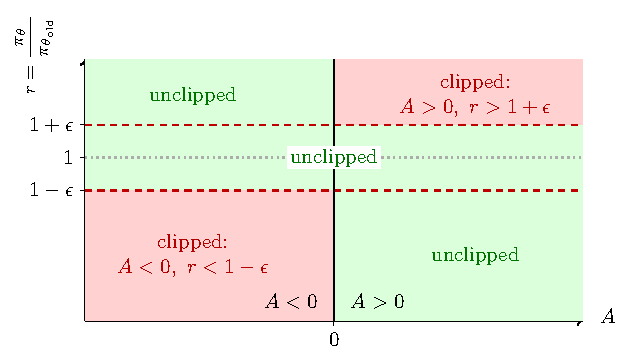
\includegraphics[width=0.7\linewidth]{figures/ppo_clip_region.pdf}
    \caption{PPO-Clip trust region in the $(A,r)$ plane, where $r=\pi_\theta(a|s)/\pi_{\theta_{\text{old}}}(a|s)$. The red region is the clipped region, and the green region is the unclipped region (after the clip and min operation).}
    \label{fig:ppo.clip.region}
\end{figure}

\textbf{Remark}
\begin{itemize}
    \item The popular choice of $\hat A_\phi(s_t,a_t)$ is $A^{\operatorname{GAE}(\gamma, \lambda)}_{\phi} = \sum_{\ell=0}^{T-1-t}(\gamma\lambda)^{\ell}\left(r_{t+\ell} + \gamma V^{\pi}_{\phi}(s_{t+1+\ell}) - V^{\pi}_{\phi}(s_{t+\ell}) \right)$.
    \item When $\hat A_\phi(s_t,a_t)>0$, which means that $a_t$ is better than the average, we want to increase its probability. However, we need to limit the increase to not being greater than the factor of $1+\epsilon$.
     \item When $\hat A_\phi(s_t,a_t)<0$, which means that $a_t$ is worse than the average, we want to decrease its probability. However, we need to limit the decrease to be no greater than the factor of $1-\epsilon$.
    
\end{itemize}

One can also constraint the distribution shift by
\begin{align}
     \max_{\theta} \Jcal_{\text{PPO-KL}}(\theta):= \Embb_{\tau\sim \pi_{\theta_{\text{old}}}}\left[ \sum_{t=0}^{T-1} \frac{\pi_{\theta}(a_t|s_t)}{\pi_{\theta_{\text{old}}}(a_t|s_t)} \hat  A_\phi(s_t,a_t) - \beta \operatorname{K L}\left[\pi_{\theta_{\text{old}}}(\cdot|s_t) || \pi_{\theta}(\cdot|s_t)\right]\right],
\end{align}

\textbf{Remark}
\begin{itemize}
    \item When maximize $\Jcal_{\text{PPO-KL}}(\theta)$, we minimize $\mathbb{D}_{K L}\left[\pi_{\theta_{\text{old}}}(\cdot|s_t)| | \pi_{\theta}(\cdot|s_t)\right]$, i.e., we minimize the forward KL, which has the \href{https://www.tuananhle.co.uk/notes/reverse-forward-kl.html}{mean-seeking behavior}.
\end{itemize}

% There's one missing piece though. How should we update the value (critic) network? Similar to objective funciton \eqref{eq:naive.critic.obj}, the $V^{\pi}_{\phi}$ can be updated by

% \begin{align}
%      \min \left\{\Lcal(\phi):= \Embb_{\tau\sim \pi_{\theta}}\left[ \sum_{t=0}^{T-1}(r_t+\gamma V^{\pi}_{\phi_{\text{old}}}(s_{t+1}) - V^{\pi}_{\phi}(s_t)\right]\right\}.
%      \label{eq:ppo.critic.obj},
% \end{align}
% where $V^{\pi}_{\phi_{\text{old}}}$ is the value network paired with $\pi_{\theta_{\text{old}}}$. There could be other variants for t

To put pieces together, we summarize the PPO-Clip in Algorithm~\ref{algo:ppo}.
\begin{algorithm}[H]
\caption{PPO-Clip Algorithm}
\begin{algorithmic}[1]
    \State Inputs: Initial Policy network parameter $\theta_0$ and value function parameter $\phi_0$.
    \For{k=0,1,2....}
        \State Collect a set of trajectories $D_k=\{\tau_n\}_{n=1}^{N}$.
        \State Reward-to-go calculation $G_t(\tau_n) = \sum_{t'=t}^{T_n-1}\gamma^{t'-t}r_{t'}$ for all $n$.
         \State GAE calculation $A^{\operatorname{GAE(\gamma,\lambda)}}_{\phi_k}(s_t^{(n)},a_t^{(n)})$ for all $t$ and $n$\footnote{Here $(s_t^{(n)},a_t^{(n)})$ means the state and action from t-step and n-th trajectory.}. 
        \State Approximately solve 
            \begin{align*}
                 \theta_{k+1}=\arg\max_{\theta} \frac{1}{N}\sum_{n=1}^{N}\frac{1}{T_n}
                  \sum_{t=0}^{T_n-1}  
                 \min\left\{\frac{\pi_{\theta}(a_t^{(n)}|s_t^{(n)})}{\pi_{\theta_{k}}(a_t^{(n)}|s_t^{(n)})}A^{\operatorname{GAE(\gamma,\lambda)}}_{\phi_k}(s_t^{(n)},a_t^{(n)}),  \right.
                 \\
                 \left.\operatorname{clip}\left(\frac{\pi_{\theta}(a_t|s_t)}{\pi_{\theta_{k}}(a_t|s_t)}, 1-\epsilon, 1+\epsilon\right)
                 A^{\operatorname{GAE(\gamma,\lambda)}}_{\phi_k}(s_t^{(n)},a_t^{(n)})\right\},
            \end{align*}
        \State Approximately solve 
            \begin{align*}
                \phi_{k+1}=\arg\min_{\phi} \frac{1}{N}\sum_{n=1}^{N}\frac{1}{T_n}
                  \sum_{t=0}^{T_n-1}(V^{\pi}_{\phi}(s_t^{(n)}) - G_t(\tau_n))^2
            \end{align*}
    \EndFor
\end{algorithmic}
\label{algo:ppo}
\end{algorithm}

\subsection{PPO in the context of RLHF}
Let us first introduce a new set of notions and setup. Let $\Dcal$ be a set of prompt and $x\in\Dcal$ is any sample from it. $y\sim \pi_{\theta}(\cdot|x)$ be a response sampled from the policy model $\pi_{\theta}$ given the prompt $x$. To simplify the discussion, let us assume that the reward model is given and we focus on the outcome reward $r(x,y)$. 

We consider the following variant objective function inspired by policy gradient and PPO
\begin{align*}
   \Jcal(\theta) = \Embb_{x\sim \Dcal, y\sim\pi_{\theta}(\cdot|x)} \left[ r(x,y) - \beta \operatorname{KL}\left[\pi_{\theta}(\cdot|x) || \pi_{\theta_{\text{ref}}}(\cdot|x)\right]\right],
\end{align*}
note that here we used forward KL divergence.
Then the gradient is 
\begin{align}\label{eq:RLHF.gradient.part1}
\grad \Jcal(\theta) = \int_{x\in \Xcal} p(x)\left\{\left[\int_{y\in\Ycal(x)}r(x,y)\frac{\partial}{\partial \theta}\pi_{\theta}(y|x)dy\right] - \beta \left[\int_{s\in\Ycal(x)}\frac{\partial}{\partial\theta}\pi_{\theta}(s|x)\log\frac{\pi_{\theta}(s|x)}{\pi_{\theta_{\text{ref}}}(y|x)}ds\right] \right\}dx,
\end{align}
where $\Xcal=\Dcal$ and $\Ycal(x)=\text{support}(\pi_{\theta}(y|x))$.
Note that
\begin{align}
    & \int_{s\in\Ycal(x)}\frac{\partial}{\partial\theta}\pi_{\theta}(s|x)\log\frac{\pi_{\theta}(s|x)}{\pi_{\theta_{\text{ref}}}(s|x)}ds  \nonumber\\
    & =  \int_{s\in\Ycal(x)}\left[\grad\pi_{\theta}(s|x)\cdot\log\frac{\pi_{\theta}(s|x)}{\pi_{\theta_{\text{ref}}}(s|x)} + \pi_{\theta}(s|x)\cdot \grad\log\frac{\pi_{\theta}(s|x)}{\pi_{\theta_{\text{ref}}}(s|x)}\right]ds \nonumber\\
    & = \int_{s\in\Ycal(x)}\left[\grad\pi_{\theta}(s|x)\cdot\log\frac{\pi_{\theta}(s|x)}{\pi_{\theta_{\text{ref}}}(s|x)} + \grad \pi_{\theta}(s|x)\right]ds \nonumber\\
    & = \int_{s\in\Ycal(x)}\grad\pi_{\theta}(s|x)\cdot\log\frac{\pi_{\theta}(s|x)}{\pi_{\theta_{\text{ref}}}(s|x)} ds \label{eq:RLHF.gradient.part2}
\end{align}  
where the last line follows from \eqref{eq:grad.log.prob}. Combining \eqref{eq:RLHF.gradient.part1} and \eqref{eq:RLHF.gradient.part2}, one obtains
\begin{align}\label{eq:RLHF.gradient.part3}
\grad \Jcal(\theta)
 & = \int_{x\in \Xcal} p(x)\left\{\left[\int_{y\in\Ycal(x)}r(x,y)\frac{\partial}{\partial \theta}\pi_{\theta}(y|x)dy\right] - \beta \left[\int_{s\in\Ycal(x)}\grad\pi_{\theta}(s|x)\cdot\log\frac{\pi_{\theta}(s|x)}{\pi_{\theta_{\text{ref}}}(s|x)} ds\right] \right\}dx \nonumber\\
 & = \int_{x\in \Xcal, y\in\Ycal(x)} p(x)\left\{ \pi_{\theta}(y|x) \left[ r(x,y)\grad\log \pi_{\theta}(y|x) - \beta\grad\log\pi_{\theta}(y|x)\cdot\log\frac{\pi_{\theta}(y|x)}{\pi_{\theta_{\text{ref}}}(y|x)}\right]  \right\}dydx \nonumber\\
 & = \Embb_{x\sim \Dcal, y\sim\pi_{\theta}(\cdot|x)}\left[\left(r(x,y) - \beta\log\frac{\pi_{\theta}(y|x)}{\pi_{\theta_{\text{ref}}}(y|x)}\right)\grad\log\pi_{\theta}(y|x)\right]
\end{align}
From \eqref{eq:RLHF.gradient.part3}, we conclude the "PPO" version of the RLHF objective function
\begin{align}\label{eq:rlhf.obj}
  \max_{\theta} \Jcal_{\text{RLHF}}(\theta):=\Embb_{x\sim \Dcal, y\sim\pi_{\theta}(\cdot|x)}\left[r(x,y) - \beta\log\frac{\pi_{\theta}(y|x)}{\pi_{\theta_{\text{ref}}}(y|x)}\right],
\end{align}
which recovers the first part of the objective function in Equation (2) of \citet{ouyang2022training}.
\section{REINFORCE++}



REINFORCE++ modifies PPO in the LLM text by introducing
\begin{itemize}
    % \item using outcome reward model $r(x,y)$, where $x$ and $y$ are input prompt and response, respectively;
    \item token-level KL penalty  $\operatorname{KL}(t;\theta)=\log\frac{\pi_{\theta}(a_t|s_t)}{\pi_{\theta_{\text{ref}}}(a_t|s_t)}$, where $\pi_{\theta_{\text{ref}}}$ can be the SFT model;
    \item token-level reward function $r_t=\Imbb(s_t=[\text{EOS}])r(x,y)-\beta\operatorname{KL}(t)$, where $x$ and $y$ are input prompt and response, respectively and $r(x,y)$ is the outcome reward.
\end{itemize}

Recall the advantage used in PPO is $A^{\operatorname{GAE}(\gamma, \lambda)}_{\phi} = \sum_{\ell=0}^{T-1-t}(\gamma\lambda)^{\ell}\left(r_{t+\ell} + \gamma V^{\pi}_{\phi}(s_{t+1+\ell}) - V^{\pi}_{\phi}(s_{t+\ell}) \right)$. If we drop the value network and plug in the new definition of $r_t$, we get 

\begin{align*}
    A^{\operatorname{GAE}(\gamma, \lambda)}_{t} 
    & = \sum_{\ell=0}^{T-1-t}(\gamma\lambda)^{\ell}\left[\Imbb(s_{t+\ell}=[\text{EOS}])r(x,y)-\beta\operatorname{KL}(t+\ell;\theta) \right] \\
    & = \sum_{i=t}^{T-1}(\gamma\lambda)^{\ell}\left[\Imbb(s_{i}=[\text{EOS}])r(x,y)-\beta\operatorname{KL}(i) \right]  = (\gamma\lambda)^{T-1}r(x,y)-\sum_{i=t}^{T-1}(\gamma\lambda)^{i}\left[\beta\operatorname{KL}(i;\theta) \right].
\end{align*}
Specifically, letting $\gamma=\lambda=1$, we get the advantage estimation used in REINFORCE++ as
\begin{equation}
A^{\operatorname{RF++}}_{t}=r(x,y) - \sum_{i=t}^{T-1}\beta\operatorname{KL}(i;\theta). 
\end{equation}


Consequently, for the $k$th episode, REINFORCE++ solves the following problem

\begin{align*}
     \theta_{k+1}=\arg\max_{\theta} \frac{1}{N}\sum_{n=1}^{N}\frac{1}{T_n}
      \sum_{t=0}^{T_n-1}  
     \min\left\{\frac{\pi_{\theta}(a_t^{(n)}|s_t^{(n)})}{\pi_{\theta_{k}}(a_t^{(n)}|s_t^{(n)})}\bar A_{n,t}, \operatorname{clip}\left(\frac{\pi_{\theta}(a_t|s_t)}{\pi_{\theta_{k}}(a_t|s_t)}, 1-\epsilon, 1+\epsilon\right)
     \bar A_{n,t}\right\},
\end{align*}
where $\bar A_{n,t} = \frac{A^{\operatorname{RF++}}_{n,t}-\mu_k}{\sigma_k}$, $\mu_k=\operatorname{mean}\{A^{\operatorname{RF++}}_{n,t}\}_{n\in[1,N], t\in[0,T_n-1]}$, $\sigma_k=\operatorname{std}\{A^{\operatorname{RF++}}_{n,t}\}_{n\in[1,N], t\in[0,T_n-1]}$, $A^{\operatorname{RF++}}_{n,t}=r(x^{(n)},y^{(n)}) - \sum_{i=t}^{T_n-1}\beta\operatorname{KL}(i;\theta_k)$, and $(x^{(n)},y^{(n)})$ is the $n$th sample.

To conclude, we summarize REINFORCE++ in Algorithm~\ref{algo:RF++}.
\begin{algorithm}[H]
\caption{REINFORCE++}
\begin{algorithmic}[1]
    \State Inputs: Initial Policy network parameter $\theta_0$.
    \For{k=0,1,2....}
        \State Collect a set of trajectories $D_k=\{\tau_n\}_{n=1}^{N}$.
        \State $\{A_{n,t}^{\text{RF++}}\}_{n\in[1,N], t\in[0,T_n-1]}$ calculation, batch mean $\mu_k$ and variance $\sigma_k$  calculation.
        \State Compute normalized advantage estimation $\{\bar A_{n,t} = \frac{A^{\operatorname{RF++}}_{n,t}-\mu_k}{\sigma_k}\}_{n\in[1,N], t\in[0,T_n-1]}$.
        \State Approximately solve 
            \begin{align*}
                 \theta_{k+1}=\arg\max_{\theta} \frac{1}{N}\sum_{n=1}^{N}\frac{1}{T_n}
                  \sum_{t=0}^{T_n-1}  
                 \min\left\{\frac{\pi_{\theta}(a_t^{(n)}|s_t^{(n)})}{\pi_{\theta_{k}}(a_t^{(n)}|s_t^{(n)})}\bar A_{n,t}, \operatorname{clip}\left(\frac{\pi_{\theta}(a_t|s_t)}{\pi_{\theta_{k}}(a_t|s_t)}, 1-\epsilon, 1+\epsilon\right)
                 \bar A_{n,t}\right\},                 
            \end{align*}
    \EndFor
\end{algorithmic}
\label{algo:RF++}
\end{algorithm}


\textbf{Remark}
\begin{itemize}
    \item Compared to GRPO, the normalization happens on the "batch" level; while GRPO applies the normalization within the "group" level.
    \item The KL penalty applied in the loss function is different. For GRPO, the KL penalty is taken out of the definition of the advantage estimation and uses the $k_3$ estimator (recall the definition in Definition\ref{def:kl-est}), which is 
    $\beta\mathbb{D}_{K L}\left[\pi_\theta| | \pi_{\text{ref}}\right](i,t)$
   . In REINFORCE++, the $\operatorname{KL}$ penalty is factorized in the definition of the advantage estimation and uses the $k_1$ estimator, which is  $\beta\sum_{i=t}^{T-1}\operatorname{KL}(i;\theta)$. Notice that in the $t$th action, the penalty is the accumulation of all $\operatorname{KL}$ penalties starting from the time step $t$ to the end.
\end{itemize}

Motivated by the discussion above, \citet{xie2025logic} modifies the loss function by combining the GRPO and REINFROCE++ as below.

 \begin{align*}
     \theta_{k+1}=\arg\max_{\theta} \frac{1}{N}\sum_{n=1}^{N}\frac{1}{T_n}
      \sum_{t=0}^{T_n-1}  
     \min\left\{\frac{\pi_{\theta}(a_t^{(n)}|s_t^{(n)})}{\pi_{\theta_{k}}(a_t^{(n)}|s_t^{(n)})}\bar A_{n,t}, \operatorname{clip}\left(\frac{\pi_{\theta}(a_t|s_t)}{\pi_{\theta_{k}}(a_t|s_t)}, 1-\epsilon, 1+\epsilon\right)
     \bar A_{n,t} -\beta \mathbb{D}_{K L}\left[\pi_\theta| | \pi_{\text{ref}}\right](i,t)\right\},                 
\end{align*}
where $\bar A_{n,t} = \frac{A^{\operatorname{Logic}}_{n,t}-\mu_k}{\sigma_k}$, $\mu_k=\operatorname{mean}\{A^{\operatorname{Logic}}_{n,t}\}_{n\in[1,N], t\in[0,T_n-1]}$, $\sigma_k=\operatorname{std}\{A^{\operatorname{Logic}}_{n,t}\}_{n\in[1,N], t\in[0,T_n-1]}$, $A^{\operatorname{Logic}}_{n,t}=r(x^{(n)},y^{(n)})$. Basically, it moves $\operatorname{KL}$ penalty out of the definition of the advantage estimators and use $k_3$ $\operatorname{KL}$  estimation.



\section{Implicit Reward in Direct Preference Optimization}

Direct Preference Optimization (DPO) does not explicitly train a separate reward model. Instead, it implicitly defines a reward function through the relationship between the optimized policy and the reference policy.

DPO can be derived from the KL-regularized RLHF objective:
\[
    \max_{\pi}
    \mathbb{E}_{y\sim \pi(\cdot\mid x)}
    \left[
        r(x,y)
    \right]
    -
    \beta
    D_{\mathrm{KL}}
    \left(
        \pi(\cdot\mid x)
        \middle\|
        \pi_{\mathrm{ref}}(\cdot\mid x)
    \right),
\]
where $\pi_{\mathrm{ref}}$ is a fixed reference policy, usually the supervised fine-tuned model, and $\beta>0$ controls the strength of the KL regularization.

The optimal policy of this objective satisfies
\[
    \pi^\star(y\mid x)
    =
    \frac{1}{Z(x)}
    \pi_{\mathrm{ref}}(y\mid x)
    \exp
    \left(
        \frac{1}{\beta} r(x,y)
    \right),
\]
where $Z(x)$ is the partition function depending only on the prompt $x$.

Solving for the reward gives
\[
    r(x,y)
    =
    \beta
    \log
    \frac{
        \pi^\star(y\mid x)
    }{
        \pi_{\mathrm{ref}}(y\mid x)
    }
    +
    \beta \log Z(x).
\]
Since $\beta\log Z(x)$ depends only on the prompt $x$, it cancels when comparing two responses to the same prompt. Therefore, DPO uses the following implicit reward parameterization:
\[
    r_\theta(x,y)
    =
    \beta
    \log
    \frac{
        \pi_\theta(y\mid x)
    }{
        \pi_{\mathrm{ref}}(y\mid x)
    }
    +
    C(x),
\]
where $C(x)$ is a prompt-dependent constant.

For a preferred response $y_w$ and a rejected response $y_l$, the reward difference is
\[
\begin{aligned}
    r_\theta(x,y_w)-r_\theta(x,y_l)
    &=
    \beta
    \left[
        \log
        \frac{
            \pi_\theta(y_w\mid x)
        }{
            \pi_{\mathrm{ref}}(y_w\mid x)
        }
        -
        \log
        \frac{
            \pi_\theta(y_l\mid x)
        }{
            \pi_{\mathrm{ref}}(y_l\mid x)
        }
    \right] \\
    &=
    \beta
    \left[
        \log \pi_\theta(y_w\mid x)
        -
        \log \pi_\theta(y_l\mid x)
        -
        \log \pi_{\mathrm{ref}}(y_w\mid x)
        +
        \log \pi_{\mathrm{ref}}(y_l\mid x)
    \right].
\end{aligned}
\]
Thus, the implicit reward in DPO measures how much the optimized policy increases the probability of a response relative to the reference policy.

\subsection{DPO Objective}

DPO is trained on preference data of the form
\[
    (x,y_w,y_l)\sim \mathcal{D},
\]
where $x$ is the prompt, $y_w$ is the preferred response, and $y_l$ is the rejected response.

The DPO loss is
\[
    \mathcal{L}_{\mathrm{DPO}}(\theta)
    =
    -
    \mathbb{E}_{(x,y_w,y_l)\sim\mathcal{D}}
    \left[
        \log \sigma
        \left(
            \beta
            \left[
                \log
                \frac{
                    \pi_\theta(y_w\mid x)
                }{
                    \pi_{\mathrm{ref}}(y_w\mid x)
                }
                -
                \log
                \frac{
                    \pi_\theta(y_l\mid x)
                }{
                    \pi_{\mathrm{ref}}(y_l\mid x)
                }
            \right]
        \right)
    \right],
\]
where $\sigma(\cdot)$ is the sigmoid function.

Define
\[
    \Delta_\theta(x,y_w,y_l)
    =
    \log
    \frac{
        \pi_\theta(y_w\mid x)
    }{
        \pi_{\mathrm{ref}}(y_w\mid x)
    }
    -
    \log
    \frac{
        \pi_\theta(y_l\mid x)
    }{
        \pi_{\mathrm{ref}}(y_l\mid x)
    }.
\]
Then the DPO loss can be written compactly as
\[
    \mathcal{L}_{\mathrm{DPO}}(\theta)
    =
    -
    \mathbb{E}_{(x,y_w,y_l)\sim\mathcal{D}}
    \left[
        \log \sigma
        \left(
            \beta \Delta_\theta(x,y_w,y_l)
        \right)
    \right].
\]

Minimizing this loss increases the relative log-probability of the preferred response over the rejected response, after correcting for their probabilities under the reference policy.

\subsection{Reward Hacking in DPO}

DPO does not use an explicit reward model during optimization. Therefore, it is less likely to suffer from the classical online reward hacking problem in PPO-style RLHF, where the policy repeatedly exploits weaknesses of a learned reward model.

However, DPO can still suffer from a different form of reward hacking or over-optimization. Since the implicit reward is determined by the preference dataset,
\[
    (x,y_w,y_l)\sim \mathcal{D},
\]
DPO may exploit biases or artifacts in the preference data.

In this sense, DPO does not hack an explicit reward model. Instead, it may overfit or exploit the implicit preference signal encoded in the dataset:
\[
    \text{DPO may hack the preference dataset rather than a learned reward model.}
\]

For example, if preferred responses are systematically longer than rejected responses, the model may learn the spurious rule
\[
    \text{longer response} \Rightarrow \text{better response}.
\]
If preferred responses often contain certain stylistic patterns, the model may learn to imitate those patterns even when they do not improve semantic quality.

Thus, DPO can still exhibit reward-hacking-like behavior through preference-data bias, distribution shift, or over-optimization of the implicit reward.

\subsection{Common Failure Modes of DPO}

A common failure mode of DPO is length bias. The sequence log-probability is
\[
    \log \pi_\theta(y\mid x)
    =
    \sum_{t=1}^{|y|}
    \log \pi_\theta(y_t\mid x,y_{<t}).
\]
If preferred responses are usually longer than rejected responses, the model may learn to favor longer responses, even when they are not more accurate or helpful.

Another failure mode is style bias. If preferred responses share superficial stylistic features, such as excessive politeness, rigid formatting, or repeated templates, DPO may learn these features as proxies for quality.

DPO may also overfit to easy negatives. If the rejected response $y_l$ is much worse than the preferred response $y_w$, the model only learns a coarse distinction:
\[
    y_w \gg y_l.
\]
This may not teach the model how to distinguish between two high-quality responses.

Finally, DPO is an offline preference optimization method. It is trained on fixed preference data, but after training, the model generates responses from its own policy:
\[
    y\sim \pi_\theta(\cdot\mid x).
\]
If this generation distribution differs significantly from the training preference data distribution, DPO may suffer from distribution shift.

\subsection{Mitigating Reward Hacking and Over-Optimization in DPO}

One important mitigation is improving the quality of the preference data. The preference dataset should minimize spurious correlations between preference labels and superficial features such as length, format, or style. Ideally, the preference label should reflect semantic quality rather than dataset artifacts.

To reduce length bias, one can use length-normalized log-probabilities. Instead of using
\[
    \log \pi_\theta(y\mid x)
    =
    \sum_{t=1}^{|y|}
    \log \pi_\theta(y_t\mid x,y_{<t}),
\]
one may use the average log-probability
\[
    \frac{1}{|y|}
    \log \pi_\theta(y\mid x)
    =
    \frac{1}{|y|}
    \sum_{t=1}^{|y|}
    \log \pi_\theta(y_t\mid x,y_{<t}).
\]

Another mitigation is tuning the temperature parameter $\beta$. The parameter $\beta$ controls the strength of the preference margin in the DPO loss:
\[
    \log \sigma
    \left(
        \beta \Delta_\theta(x,y_w,y_l)
    \right).
\]
If $\beta$ is too large, the optimization may aggressively separate preferred and rejected responses, increasing the risk of over-optimization. A smaller $\beta$ makes the update more conservative.

One can also monitor or explicitly regularize the divergence from the reference model:
\[
    D_{\mathrm{KL}}
    \left(
        \pi_\theta
        \middle\|
        \pi_{\mathrm{ref}}
    \right).
\]
Although DPO already uses the reference policy in its objective, explicit KL monitoring or early stopping can help prevent excessive drift from the reference model.

Another practical method is to mix the DPO loss with a supervised fine-tuning loss:
\[
    \mathcal{L}(\theta)
    =
    \mathcal{L}_{\mathrm{DPO}}(\theta)
    +
    \lambda_{\mathrm{SFT}}
    \mathcal{L}_{\mathrm{SFT}}(\theta),
\]
where
\[
    \mathcal{L}_{\mathrm{SFT}}(\theta)
    =
    -
    \mathbb{E}_{(x,y_w)\sim\mathcal{D}}
    \left[
        \log \pi_\theta(y_w\mid x)
    \right].
\]
The SFT loss helps preserve language quality, instruction-following behavior, and formatting stability.

Finally, iterative preference data collection can reduce distribution shift. Instead of training only on a fixed offline dataset, one can repeatedly sample responses from the current policy,
\[
    y\sim \pi_\theta(\cdot\mid x),
\]
collect new preference labels, and continue preference optimization on data closer to the current model distribution.
\section{Group Relative Policy Optimization}

GRPO is motivated by removing the requirements on estimating the value function is ued PPO Algorithm~\ref{algo:ppo}.


For each question $q\sim P(Q)$, GRPO samples a group of outputs $\{o_1, o_2, \ldots, o_G\}$ from the old policy $\pi_{\theta_{\text{old}}}$.
\begin{align}
& \Jcal_{GRPO}(\theta) \nonumber =\Embb_{\left[q \sim P(Q),\left\{o_i\right\}_{i=1}^G \sim \pi_{\theta_{\text{old}}}(O | q)\right]} \nonumber\\
& \left[\frac{1}{G} \sum_{i=1}^G \frac{1}{\left|o_i\right|} \sum_{t=1}^{\left|o_i\right|}\left\{ \min\left[\frac{\pi_\theta\left(o_{i, t} | q, o_{i,<t}\right)}{\pi_{\theta_{\text{old}}}\left(o_{i, t} | q, o_{i,<t}\right)}\hat{A}_{i, t}, \operatorname{clip}\left(\frac{\pi_\theta\left(o_{i, t} | q, o_{i,<t}\right)}{\pi_{\theta_{o l d}}\left(o_{i, t} | q, o_{i,<t}\right)}, 1-\varepsilon, 1+\varepsilon\right) \hat{A}_{i, t}\right]-\beta \mathbb{D}_{K L}\left[\pi_\theta| | \pi_{\text{ref}}\right](i,t)\right\}\right],
\end{align}

where
\begin{itemize}
    \item $\mathbb{D}_{KL}\left[\pi_\theta| | \pi_{\text{ref}}\right]$ is the $k_3$ estimator of the KL divergence with 
    $$ 
        \mathbb{D}_{K L}\left[\pi_\theta| | \pi_{\text{ref}}\right](i,t)=\frac{\pi_{\text{ref}}\left(o_{i, t} | q, o_{i,<t}\right)}{\pi_\theta\left(o_{i, t} | q, o_{i,<t}\right)}-\log \frac{\pi_{\text{ref}}\left(o_{i, t} | q, o_{i,<t}\right)}{\pi_\theta\left(o_{i, t} | q, o_{i,<t}\right)}-1
    $$
    \item the advantage estimate is defined as $\hat{A}_{i, t}:= \frac{r_i-\operatorname{mean}(\textbf{r})}{\operatorname{std}(\textbf{r})}$ with $\textbf{r}=\{r_1, r_2, \dots, r_G\}$.
\end{itemize}

\textbf{Remark}
\begin{itemize}
    \item The reverse KL divergence is used, which has the mode-seeking behavior. The usage of $k_3$ estimator is crucial for GRPO because $k_3$ guarantee to be non-negative. Otherwise, if one adopts the $k_1$ estimator, then there could be a possibility to "hack" the training process by making the $k_1$ estimator arbitrarily small (very negative), then the reward is $\Jcal_{GRPO}(\theta)$ is also maimized. However, this means that $\pi_\theta$ is very different from  $\pi_{\text{ref}}$.  At the same time, numerical instability is observed during the training dynamics. Because the computation of $\exp \left(\frac{\pi_{\text{ref}}\left(o_{i, t} | q, o_{i,<t}\right)}{\pi_\theta\left(o_{i, t} | q, o_{i,<t}\right)}\right)$ can be unstable.
    \item In the computation of the KL term, note that $o_i\sim \pi_{\theta_{\text{old}}}$. But the link suggests that $o_i$ should be sampled from $\pi_\theta$ to make $\mathbb{D}_{K L}\left[\pi_\theta| | \pi_{\text{ref}}\right]$ an unbiased estimator. In practice, to make these make sense, one has to initialize $\pi_\theta :=\pi_{\theta_{\text{old}}}$ and take only one step update.
    \item When optimize the objective function, one of tries to $\min_{\theta} -\Jcal_{GRPO}(\theta)$. One should notice that $-\Jcal_{GRPO}$ can be smaller than $0$, meaning the loss can be negative. This could happen when "min" term is larger that the KL term, i.e., when either the two distributions are quite different or the advantage is large.
    % \item The definition of the (normalized) advantage estimation is different from that used in PPO, which drops the $\operatorname{KL}$ penalty. 
\end{itemize}
\section{Group Sequence Policy Optimization}

In GRPO, the token-level importance sampling weight $\frac{\pi_\theta\left(o_{i, t} | q, o_{i,<t}\right)}{\pi_{\theta_{\text{old}}}\left(o_{i, t} | q, o_{i,<t}\right)}$ is applied. 

GSPO argues that this is problematic since this weight  is based on a single sample $o_{i,t}$ from each next-token distribution $\pi_{\theta_{\text{old}}}\left(o_{i, t} | q, o_{i,<t}\right)$, it fails to perform  the intended distribution-correction role\footnote{Recall that Importance sampling needs multiple samples from the same distribution to reduce variance.}. Instead, it introduces high-variance noise into the training gradients, which accumulates over long sequences and is exacerbated by the clipping mechanism.

Therefore, GSPO proposes to use the sequence-level importance weight $\frac{\pi_\theta\left(o_{i} | q\right)}{\pi_{\theta_{\text{old}}}\left(o_{i} | q\right)}$. Therefore, the loss function becomes (ignoring the KL regularization term)

\begin{align}
& \Jcal_{GSPO}(\theta) \nonumber =\Embb_{\left[q \sim P(Q),\left\{o_i\right\}_{i=1}^G \sim \pi_{\theta_{\text{old}}}(O | q)\right]} \left[\frac{1}{G} \sum_{i=1}^G \min\left[s_i(\theta)\hat A_i, \operatorname{clip}\left(s_i(\theta), 1-\varepsilon, 1+\varepsilon\right) \hat{A}_{i}\right]\right],
\end{align}
where
$s_i(\theta)=(\frac{\pi_\theta\left(o_{i} | q\right)}{\pi_{\theta_{\text{old}}}\left(o_{i} | q\right)})^{1/|o_i|} = \exp\left(\frac{1}{\left|o_i\right|} \sum_{t=1}^{\left|o_i\right|}\log\left\{\frac{\pi_\theta\left(o_{i, t} | q, o_{i,<t}\right)}{\pi_{\theta_{\text{old}}}\left(o_{i, t} | q, o_{i,<t}\right)}\right\}\right)$, and $\hat A_i = \frac{r(x, o_i) - \text{mean}\left(\{r(x,o_j)\}_{j=1}^G\right)}{\text{std}\left(\{r(x,o_j)\}_{j=1}^G\right)}$.

Therefore, GSPO applies clipping to entire responses instead of individual tokens to exclude the overly "off-policy" samples from gradient estimation, which matches both the sequence-level rewarding and optimization.Also, note that the clipping ranges in GSPO and in previous algorithms (e.g., GRPO) typically differ in order of magnitude due to the distinct definitions of importance ratios.


In scenarios like multi-turn RL, we may desire a finer-grained advantage adjustment than the sequence level.
\begin{align}
& \Jcal_{GSPO-token}(\theta) \nonumber =\Embb_{\left[q \sim P(Q),\left\{o_i\right\}_{i=1}^G \sim \pi_{\theta_{\text{old}}}(O | q)\right]} \left[\frac{1}{G} \sum_{i=1}^G \frac{1}{\left|o_i\right|} \sum_{t=1}^{\left|o_i\right|}\left\{ \min\left[s_{i,t}(\theta)\hat{A}_{i, t}, \operatorname{clip}\left(s_{i,t}(\theta), 1-\varepsilon, 1+\varepsilon\right) \hat{A}_{i, t}\right]\right\}\right],
\end{align}
where $s_{i,t}(\theta) = \text{sg}[s_i(\theta)] \frac{\pi_\theta\left(o_{i, t} | q, o_{i,<t}\right)}{\text{sg}\left[\pi_{\theta}\left(o_{i, t} | q, o_{i,<t}\right)\right]}$ and $\text{sg}$ is the stop gradient operator, so numerically, $s_{i,t}(\theta) = s_i(\theta)$. 


To see more clearly about the gradient of the GSPO, GSPO-token, and GRPO, we can compute (clipping is omitted for brevity

\begin{align*}
\nabla_\theta \mathcal{J}_{\mathrm{GSPO}}(\theta)
&= \nabla_\theta \mathbb{E}_{x \sim \mathcal{D}, \{o_i\}_{i=1}^G \sim \pi_{\theta_{\text{old}}}(\cdot \mid x)}
\left[
\frac{1}{G} \sum_{i=1}^G s_i(\theta)\, \hat{A}_i
\right]  \\
&= \mathbb{E}_{x \sim \mathcal{D}, \{o_i\}_{i=1}^G \sim \pi_{\theta_{\text{old}}}(\cdot \mid x)}
\left[
\frac{1}{G} \sum_{i=1}^G s_i(\theta)\, \hat{A}_i \cdot \nabla_\theta \log s_i(\theta)
\right]  \\
&= \mathbb{E}_{x \sim \mathcal{D}, \{o_i\}_{i=1}^G \sim \pi_{\theta_{\text{old}}}(\cdot \mid x)}
\left[
\frac{1}{G} \sum_{i=1}^G 
\left(
\frac{\pi_\theta(o_i \mid x)}{\pi_{\theta_{\text{old}}}(o_i \mid x)}
\right)^{\frac{1}{|o_i|}}
\hat{A}_i \cdot \frac{1}{|o_i|} \sum_{t=1}^{|o_i|}
\nabla_\theta \log \pi_\theta(o_{i,t} \mid x, o_{i,<t})
\right] 
\end{align*}

\begin{align*}
\nabla_\theta \mathcal{J}_{\mathrm{GSPO\text{-}token}}(\theta)
&= \nabla_\theta \mathbb{E}_{x \sim \mathcal{D}, \{o_i\}_{i=1}^G \sim \pi_{\theta_{\text{old}}}(\cdot \mid x)}
\left[
\frac{1}{G} \sum_{i=1}^G \frac{1}{|o_i|} \sum_{t=1}^{|o_i|} s_{i,t}(\theta)\, \hat{A}_{i,t}
\right] \\
&= \mathbb{E}_{x \sim \mathcal{D}, \{o_i\}_{i=1}^G \sim \pi_{\theta_{\text{old}}}(\cdot \mid x)}
\left[
\frac{1}{G} \sum_{i=1}^G s_i(\theta) \cdot \frac{1}{|o_i|}
\sum_{t=1}^{|o_i|}
\hat{A}_{i,t} \frac{\nabla_\theta \pi_\theta(o_{i,t} \mid x, o_{i,<t})}
{\pi_\theta(o_{i,t} \mid x, o_{i,<t})}
\right] \\
&= \mathbb{E}_{x \sim \mathcal{D}, \{o_i\}_{i=1}^G \sim \pi_{\theta_{\text{old}}}(\cdot \mid x)}
\left[
\frac{1}{G} \sum_{i=1}^G 
\left(
\frac{\pi_\theta(o_i \mid x)}{\pi_{\theta_{\text{old}}}(o_i \mid x)}
\right)^{\frac{1}{|o_i|}}
\cdot \frac{1}{|o_i|}
\sum_{t=1}^{|o_i|}
\hat{A}_{i,t}\, \nabla_\theta \log \pi_\theta(o_{i,t} \mid x, o_{i,<t})
\right]
\end{align*}

\begin{align*}
\nabla_\theta \mathcal{J}_{\mathrm{GRPO}}(\theta)
&= \nabla_\theta \mathbb{E}_{x \sim \mathcal{D}, \{o_i\}_{i=1}^G \sim \pi_{\theta_{\text{old}}}(\cdot \mid x)}
\left[
\frac{1}{G} \sum_{i=1}^G \frac{1}{|o_i|} \sum_{t=1}^{|o_i|} w_{i,t}(\theta)\, \hat{A}_{i,t}
\right] \\
&= \mathbb{E}_{x \sim \mathcal{D}, \{o_i\}_{i=1}^G \sim \pi_{\theta_{\text{old}}}(\cdot \mid x)}
\left[
\frac{1}{G} \sum_{i=1}^G \hat{A}_i \cdot \frac{1}{|o_i|}
\sum_{t=1}^{|o_i|}
\frac{\pi_\theta(o_{i,t} \mid x, o_{i,<t})}
{\pi_{\theta_{\text{old}}}(o_{i,t} \mid x, o_{i,<t})}
\, \nabla_\theta \log \pi_\theta(o_{i,t} \mid x, o_{i,<t})
\right]
\end{align*}

Therefore, the fundamental distinction between GSPO and GRPO lies in how they weight the gradients of the log likelihoods of tokens. In GRPO, the tokens are weighted according to their respective "importance  weight". In contrast, GSPO weights all the tokens in a response equally, eliminating this instability factor of GRPO.

GSPO-token and GSPO are numerically identical in the optimization objective, clipping condition, and theoretical gradient when we set the  advantages of all the tokens in the response $o_i$ to the same value (i.e., $\hat A_{i,t} = \hat A_i$), while GSPO-token enjoys the higher flexibility of adjusting the advantages per token.


\begin{equation}
  r_{i,t} =
  \begin{cases}
    r^{\mathrm{re}}_{i,t} + \gamma^{T_i-t}R_{\text{out},i}, & R_{\mathrm{out},i}=+1,\\[4pt]
    \texttt{sim}_{i^*,t}\cdot r^{\mathrm{re}}_{i^*,t} + \gamma^{T_i-t}R_{\text{out},i}, & R_{\mathrm{out},i}=-1.
  \end{cases}
\end{equation}
\section{Clipped Importance Sampling Policy Optimization}

Clipped Importance Sampling Policy Optimization (CISPO~\citep{minimax2025minimaxm1scalingtesttimecompute}) propsed in MiniMax-M1 optimizes a policy-gradient objective using a clipped importance sampling ratio as a stop-gradient weight.

The CISPO objective is defined as
\[
\mathcal{J}_{\mathrm{CISPO}}(\theta)
=
\mathbb{E}_{(q,a)\sim \mathcal{D},\ \{o_i\}_{i=1}^{G}\sim \pi_{\theta_{\mathrm{old}}}(\cdot\mid q)}
\left[
    \frac{1}{\sum_{i=1}^{G}|o_i|}
    \sum_{i=1}^{G}
    \sum_{t=1}^{|o_i|}
    \operatorname{sg}\!\left(\hat r_{i,t}(\theta)\right)
    \hat A_{i,t}
    \log \pi_\theta(o_{i,t}\mid q,o_{i,<t})
\right].
\]

Here, $\hat A_{i,t}$ is the estimated advantage for token $o_{i,t}$, and $\operatorname{sg}(\cdot)$ denotes the stop-gradient operation. Therefore, $\operatorname{sg}\!\left(\hat r_{i,t}(\theta)\right)$ is treated as a constant when taking gradients with respect to $\theta$. The clipped importance sampling ratio is
\[
    \hat r_{i,t}(\theta)
    =
    \operatorname{clip}
    \left(
        r_{i,t}(\theta),
        1-\epsilon_{\mathrm{low}},
        1+\epsilon_{\mathrm{high}}
    \right),
\]
where the token-level importance sampling ratio is
\[
    r_{i,t}(\theta)
    =
    \frac{
        \pi_\theta(o_{i,t}\mid q,o_{i,<t})
    }{
        \pi_{\theta_{\mathrm{old}}}(o_{i,t}\mid q,o_{i,<t})
    }.
\]

Equivalently,
\[
    \hat r_{i,t}(\theta)
    =
    \begin{cases}
    1-\epsilon_{\mathrm{low}},
    &
    r_{i,t}(\theta) < 1-\epsilon_{\mathrm{low}},
    \\[4pt]
    r_{i,t}(\theta),
    &
    1-\epsilon_{\mathrm{low}}
    \leq r_{i,t}(\theta)
    \leq 1+\epsilon_{\mathrm{high}},
    \\[4pt]
    1+\epsilon_{\mathrm{high}},
    &
    r_{i,t}(\theta) > 1+\epsilon_{\mathrm{high}}.
    \end{cases}
\]

Thus, CISPO does not clip the surrogate objective itself. Instead, it clips the token-level importance sampling ratio and uses the clipped ratio as a stop-gradient coefficient in front of the log-probability term.

\subsection{Gradient Difference between PPO and CISPO}

The main difference between PPO and CISPO is how clipping affects the policy gradient.

For PPO, the clipped surrogate objective at token $(i,t)$ can be written as
\[
    L^{\mathrm{PPO}}_{i,t}(\theta)
    =
    \min
    \left(
        r_{i,t}(\theta)\hat A_{i,t},
        \operatorname{clip}
        \left(
            r_{i,t}(\theta),
            1-\epsilon,
            1+\epsilon
        \right)
        \hat A_{i,t}
    \right),
\]
where
\[
    r_{i,t}(\theta)
    =
    \frac{
        \pi_\theta(o_{i,t}\mid q,o_{i,<t})
    }{
        \pi_{\theta_{\mathrm{old}}}(o_{i,t}\mid q,o_{i,<t})
    }.
\]

Consider the case
\[
    \hat A_{i,t} > 0
    \quad \text{and} \quad
    r_{i,t}(\theta) > 1+\epsilon.
\]
Then the clipped PPO objective becomes
\[
    L^{\mathrm{PPO}}_{i,t}(\theta)
    =
    (1+\epsilon)\hat A_{i,t}.
\]
This term is constant with respect to $\theta$, and therefore
\[
    \nabla_\theta L^{\mathrm{PPO}}_{i,t}(\theta)
    =
    0.
\]
Thus, when the probability of a positive-advantage token has already increased beyond the clipping range, PPO removes the gradient contribution from this token.

Similarly, if
\[
    \hat A_{i,t} < 0
    \quad \text{and} \quad
    r_{i,t}(\theta) < 1-\epsilon,
\]
then the clipped PPO objective becomes
\[
    L^{\mathrm{PPO}}_{i,t}(\theta)
    =
    (1-\epsilon)\hat A_{i,t},
\]
which is also constant with respect to $\theta$. Hence,
\[
    \nabla_\theta L^{\mathrm{PPO}}_{i,t}(\theta)
    =
    0.
\]
In this case, PPO removes the gradient contribution when the probability of a negative-advantage token has already decreased beyond the clipping range.

By contrast, CISPO uses the clipped importance sampling ratio as a stop-gradient coefficient:
\[
    \mathcal{J}_{\mathrm{CISPO}}(\theta)
    =
    \mathbb{E}
    \left[
        \frac{1}{\sum_{i=1}^{G}|o_i|}
        \sum_{i=1}^{G}
        \sum_{t=1}^{|o_i|}
        \operatorname{sg}\!\left(\hat r_{i,t}(\theta)\right)
        \hat A_{i,t}
        \log \pi_\theta(o_{i,t}\mid q,o_{i,<t})
    \right].
\]

Since
\[
    \operatorname{sg}\!\left(\hat r_{i,t}(\theta)\right)
\]
is treated as a constant during backpropagation, the gradient of the CISPO objective is
\[
    \nabla_\theta \mathcal{J}_{\mathrm{CISPO}}(\theta)
    =
    \mathbb{E}
    \left[
        \frac{1}{\sum_{i=1}^{G}|o_i|}
        \sum_{i=1}^{G}
        \sum_{t=1}^{|o_i|}
        \operatorname{sg}\!\left(\hat r_{i,t}(\theta)\right)
        \hat A_{i,t}
        \nabla_\theta
        \log \pi_\theta(o_{i,t}\mid q,o_{i,<t})
    \right].
\]

Therefore, even when the ratio $r_{i,t}(\theta)$ falls outside the clipping interval, CISPO does not make the gradient of that token vanish. Instead, the clipped ratio $\hat r_{i,t}(\theta)$
controls the magnitude of the gradient, while the token still contributes a policy-gradient signal through
\[
    \nabla_\theta \log \pi_\theta(o_{i,t}\mid q,o_{i,<t}).
\]

In short, PPO clips the surrogate objective, which can cause clipped tokens to have zero gradient. CISPO clips the importance sampling ratio and uses it as a stop-gradient weight, so clipped tokens can still contribute to the policy gradient.
% \input{RLOO}
% \section{ReMAX}

Should we accumulate the KL penalty?
\chapter{Agentic RL}

\textbf{Off-policy distillation} trains the student on sequences generated by
another source, such as human-annotated data or outputs produced in advance by
a teacher model. Classical knowledge distillation is typically off-policy: the student learns to match
the teacher's output distribution on teacher-generated trajectories.
Informally, the student learns from model answers written by others.

\textbf{On-policy distillation} instead uses trajectories sampled online from
the student's current policy. The teacher provides token-level supervision on
these student-generated trajectories. After each student update, new
trajectories are sampled from the updated policy. In this setting, the student
produces its own answers, and the teacher evaluates how it should proceed.
 
This distinction is important because it affects \textbf{exposure bias}.
Under off-policy distillation, the student is trained primarily on high-quality
teacher or reference trajectories. During inference, however, it conditions
on its own outputs. An early mistake may move the student into a state rarely
represented in the training data, causing subsequent errors to accumulate.
Exposure bias thus arises partly from the mismatch between the
teacher/reference distribution observed during training and the
student-induced state distribution encountered during generation.

On-policy training reduces this mismatch by training on trajectories produced
by the current student policy. Even erroneous states encountered during
rollout become training examples, allowing the teacher to provide supervision
at states the student is likely to visit. This better aligns the training and
inference distributions, thereby mitigating exposure bias and compounding
errors.

On-policy training does not, however, eliminate exposure bias entirely.
Differences in teacher and student capabilities, low-quality rollouts,
distributional drift over long sequences, and optimization instability may
still create discrepancies between training and inference. More precisely,
on-policy distillation mitigates exposure bias at the data-distribution level
rather than removing it at its source. Its central advantage over purely
off-policy distillation is that the student learns not only what the teacher
would do along ideal trajectories, but also what the teacher recommends in
states reached by the student itself.

\begin{figure}[!ht]
    \centering
    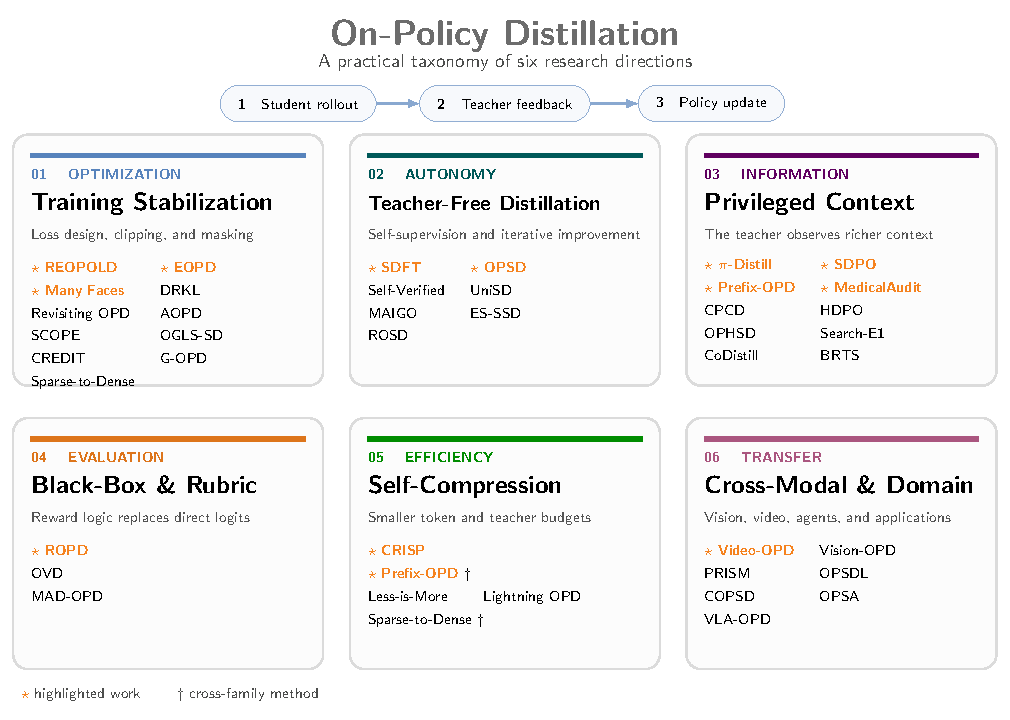
\includegraphics[width=\linewidth]{figures/opd_taxonomy.pdf}
    \caption{Six research directions in on-policy distillation, organized by the
    main source of innovation.}
    \label{fig:opd-taxonomy}
\end{figure}

\clearpage
\section{Context Compression}
\label{sec:context.compression}

\subsection{Motivation}

In a long-horizon agent rollout, the working context contains the original
instructions, model-generated actions, and environment observations.  If every
turn is appended, the context eventually reaches the model's context limit.
Even before that point, a very long context increases rollout cost and can
degrade instruction following.  Merely applying a summarizer at inference time
does not address the training problem: after old interactions are removed, the
summary determines which information is available to every subsequent action.
Summary generation is therefore part of the policy, rather than a lossless
preprocessing operation.

\subsection{Compaction Mechanism}

Both SUPO~\citep{lu2025scaling} and
CompactionRL~\citep{li2026compactionrl} make this idea trainable.  Let the
interaction history after turn $t$ be
\begin{align}
    h_t=(p_0,z_1,\ldots,z_t),
    \qquad z_i=(\ambf_i,o_i),
    \label{eq:compaction.history}
\end{align}
where $p_0$ is the fixed initial context, $\ambf_i$ is a policy-generated
assistant action span, and $o_i$ is the corresponding environment observation.
When a deterministic length threshold is reached, a fixed summarization
instruction $q_{\mathrm{sum}}$ is appended and the same trainable policy
generates
\begin{align}
    S_t\sim\pi_\theta(\cdot\mid h_t\oplus q_{\mathrm{sum}}).
    \label{eq:compaction.summary}
\end{align}
The rollout then resumes from a reconstructed context of the generic form
\begin{align}
    \bar h_t
    =
    p_{\mathrm{keep}}
    \oplus u_{\mathrm{resume}}(S_t)
    \oplus \operatorname{Tail}_\kappa(z_1,\ldots,z_t).
    \label{eq:compaction.reconstruction}
\end{align}
Here $\operatorname{Tail}_\kappa(z_1,\ldots,z_t)
=(z_{t-\kappa+1},\ldots,z_t)$ denotes the $\kappa$ most recent complete
action--observation pairs.  SUPO uses $\kappa=0$, while CompactionRL uses
$\kappa=2$ by default and reduces it when necessary to fit the context budget.  The retained
prefix $p_{\mathrm{keep}}$ is also implementation-specific.  These details do
not change the shared causal mechanism: the generated summary replaces most of
the old history and affects the terminal task reward through all future
decisions.

\begin{figure}[H]
    \centering
    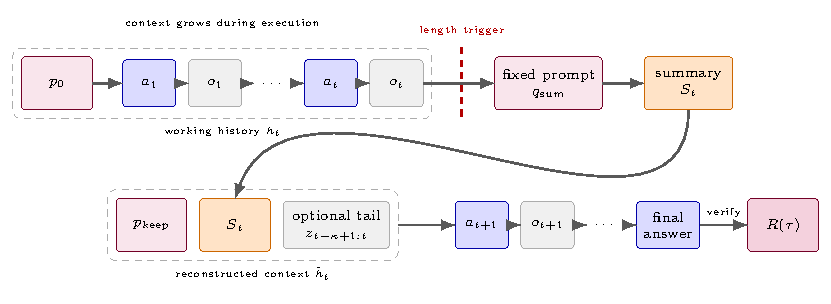
\includegraphics[width=0.98\linewidth]{figures/context_compaction_mechanism.pdf}
    \caption{Shared trainable compaction mechanism in SUPO and CompactionRL.
    A deterministic length rule triggers a fixed summary instruction, and the
    same policy that performs task actions generates the summary.  The working
    context is reconstructed from retained initial context, the summary, and an
    optional recent-history tail before the same rollout continues.  The final
    task reward trains both execution and summary tokens.  The exact retained
    prefix and history tail are method-specific.}
    \label{fig:context.compaction.mechanism}
\end{figure}

It is useful to make precise what is learned.  In both methods, the
\emph{time of compaction is forced by a length rule}; the policy does not learn
whether or when to compact.  The policy learns the summary tokens and the
ordinary execution tokens.  Partition a compacted rollout into context-bounded
multi-turn segments $\tau=(\sigma_1,\ldots,\sigma_K)$.  A typical nonfinal
segment has the form
\begin{align}
    \sigma_k
    =
    \big(
        p_{\mathrm{keep}},
        u_{\mathrm{resume}}(S_{k-1}),
        \operatorname{Tail}_{\kappa_k},
        (\ambf_{k,1},o_{k,1}),\ldots,
        (\ambf_{k,m_k},o_{k,m_k}),
        q_{\mathrm{sum}},S_k
    \big),
    \label{eq:compaction.segment}
\end{align}
where $\ambf_{k,t}$ is an assistant action span and $o_{k,t}$ is its
environment observation.  The previous summary is absent from $\sigma_1$; the
final segment omits $q_{\mathrm{sum}},S_K$ and instead ends with the final
answer.

Each assistant action span is itself a token sequence; for example,
$\ambf_{k,t}=(y_{k,t,1},\ldots,y_{k,t,L_{k,t}})$, and the summary $S_k$
also contains many policy-generated tokens.  Flatten the generated tokens in
the execution and summary spans of $\sigma_k$ in chronological order as
$y_{k,1},\ldots,y_{k,n_k}$.  Let $x_{k,i}$ be the complete visible prefix
immediately before token $y_{k,i}$ is sampled.  Thus observations are
incorporated into later prefixes $x_{k,i}$ but are not themselves optimized
tokens.  Let $\Mcal(\tau)$ collect all such policy-token coordinates $(k,i)$.
Figure~\ref{fig:compacted.rollout.indexing} visualizes this multi-turn
structure.

\begin{figure}[H]
    \centering
    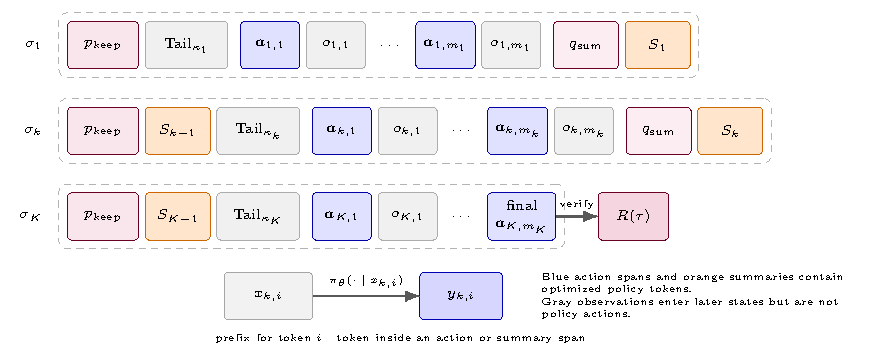
\includegraphics[width=0.98\linewidth]{figures/compacted_rollout_indexing.pdf}
    \caption{Multi-turn segment structure and policy-token indexing.  Every
    segment begins with retained context, the preceding summary when available,
    and an optional recent tail, followed by assistant action--observation
    pairs.  A nonfinal segment ends by generating its next summary.  After
    flattening only the policy-generated execution and summary tokens, $(k,i)$
    selects token $y_{k,i}$ and $x_{k,i}$ is its pre-token prefix.
    Observation tokens affect later prefixes but do not belong to
    $\Mcal(\tau)$.}
    \label{fig:compacted.rollout.indexing}
\end{figure}

With this indexing, the score-function identity gives
\begin{align}
    \grad_\theta \Jcal(\theta)
    =
    \Embb_{\tau\sim\pi_\theta}
    \left[
        R(\tau)
        \sum_{(k,i)\in\Mcal(\tau)}
        \grad_\theta\log\pi_\theta(y_{k,i}\mid x_{k,i})
    \right].
    \label{eq:compaction.policy.gradient}
\end{align}
Thus a separate summary-quality reward is not required: a summary is reinforced
when the information it preserves helps the later policy obtain a larger task
reward.  The main difference between the two algorithms is how the common
terminal reward is converted into an advantage for each token.

\subsection{CompactionRL: PPO with Cross-Segment GAE}

CompactionRL uses a fixed context budget $C$ and triggers compaction when
\begin{align}
    C-\lvert h_t\rvert<T_{\mathrm{comp}}.
\end{align}
It treats each $(\ambf_i,o_i)$ pair as atomic, so a tool call is not separated
from its observation.  After sampling $S_t$, the new context contains the
system prompt, a fixed resume template carrying $S_t$, and the $\kappa$ most
recent action--observation pairs.  The default is $\kappa=2$, reduced if needed
to fit the context budget.  We use the context-bounded segments
$\sigma_1,\ldots,\sigma_K$ defined in
Equation~\eqref{eq:compaction.segment}; execution and summary tokens in every
segment are optimized under the same rollout reward.  Here $\Mcal$ denotes all
token coordinates $(k,i)$ in these segments.

\paragraph{Token-normalized PPO objective.}
For generated token $y_{k,i}$ in $\sigma_k$, conditioned on its visible prefix
$x_{k,i}$, define the ratio against the rollout policy by
\begin{align}
    \rho_{k,i}(\theta)
    :=
    \frac{\pi_\theta(y_{k,i}\mid x_{k,i})}
         {\pi_{\theta_{\mathrm{old}}}(y_{k,i}\mid x_{k,i})}.
\end{align}
CompactionRL maximizes
\begin{align}
    \Jcal_{\mathrm{CompactionRL}}(\theta)
    :=
    \frac{1}{\lvert\Mcal\rvert}
    \sum_{(k,i)\in\Mcal}
    \min\left\{
        \rho_{k,i}(\theta)\widehat A_{k,i},
        \operatorname{clip}\left(
            \rho_{k,i}(\theta),1-\epsilon,1+\epsilon
        \right)\widehat A_{k,i}
    \right\}.
    \label{eq:compactionrl.objective}
\end{align}
The single denominator counts all optimized tokens in the batch.  This avoids
giving every compacted segment equal weight regardless of its length, which
would over-weight rollouts split into many short segments.  It does not make
all rollouts equally weighted: a rollout containing more optimized tokens can
still contribute more terms.

\paragraph{Cross-segment generalized advantage estimation.}
Let segment $\sigma_k$ contain $n_k$ optimized tokens.  CompactionRL first
computes a local GAE
\begin{align}
    \delta_{k,i}
    &:=
    r_{k,i}
    +\gamma V_\phi(x_{k,i+1})
    -V_\phi(x_{k,i}), \\
    A_{k,i}^{\mathrm{loc}}
    &:=
    \sum_{\ell=0}^{n_k-i}
    (\gamma\lambda)^\ell\delta_{k,i+\ell}.
    \label{eq:compactionrl.local.gae}
\end{align}
If this calculation is performed independently on every segment, placing the
shared terminal reward at every segment boundary would make that reward appear
too close to tokens in early segments.  Let
\begin{align}
    N_{>k}:=\sum_{m>k}n_m
\end{align}
be the number of optimized tokens in later segments of the same rollout.
CompactionRL corrects the local estimate by
\begin{align}
    \widehat A_{k,i}
    :=
    (\gamma\lambda)^{N_{>k}}A_{k,i}^{\mathrm{loc}}.
    \label{eq:compactionrl.cross.gae}
\end{align}
In particular, the terminal-reward contribution at token $(k,i)$ is
discounted by
$(\gamma\lambda)^{N_{>k}+n_k-i}$, matching its token distance to the final
outcome in the concatenated rollout.  This exact-distance statement concerns
the terminal-reward term: Equation~\eqref{eq:compactionrl.cross.gae} rescales
the entire local advantage, including its value residuals, so it is an
approximation rather than ordinary GAE over one uninterrupted state sequence.
The paper also does not fully specify the token-level placement of
$r_{k,i}$ or whether the value-regression target uses the local or corrected
advantage.

A critic $V_\phi$ is trained with the standard PPO value-regression loss, so
the method can estimate token-dependent advantages even with one rollout per
prompt.  In the reported implementation, the critic is pretrained and receives
two updates per policy update.  It uses
\begin{align}
    \lambda=1-\frac{1}{\alpha l},
    \qquad \alpha=1.5,
\end{align}
where the paper calls $l$ the response length but does not specify its exact
interpretation across multi-response execution segments.

\subsection{SUPO: GRPO with Rollout-Level Group Advantages}

SUPO augments a multi-turn tool-use MDP with a length threshold $L$.  Once the
threshold is crossed, the policy is prompted to summarize the current
subtrajectory.  The next subtrajectory starts from the original prompt plus
that summary; unlike CompactionRL, no recent action--observation tail is kept.
The practical rollout algorithm also discards the action--observation pair
that caused the threshold crossing before requesting the summary.  This keeps
the summary itself within the training context limit; the paper's theoretical
transition, in contrast, retains that pair.  A complete rollout
$\tau^j$ with $I^j$ summaries is consequently stored as $I^j+1$
subtrajectories.

\paragraph{Advantage estimation before splitting.}
For each prompt, SUPO samples $G$ complete compacted rollouts from
$\pi_{\theta_{\mathrm{old}}}$ and obtains terminal rewards
$\{R^1,\ldots,R^G\}$.  Its GRPO-style advantage is computed over these
original rollouts:
\begin{align}
    \widehat A^j
    :=
    \frac{
        R^j-\operatorname{mean}(\{R^{j'}\}_{j'=1}^{G})
    }{
        \operatorname{std}(\{R^{j'}\}_{j'=1}^{G})
    }.
    \label{eq:supo.advantage}
\end{align}
The same scalar $\widehat A^j$ is then assigned to every execution and summary
token in all $I^j+1$ subtrajectories originating from rollout $j$.  The
important detail is that $R^j$ appears only once in the group statistics.
Computing the mean and standard deviation after splitting would repeat $R^j$
$I^j+1$ times and bias the baseline toward rollouts that compact more often.
As with ordinary GRPO, the implementation must handle a group whose rewards
have zero standard deviation, but the paper does not state the safeguard used.

\paragraph{SUPO objective and overlong mask.}
Write response span $\ambf_t^j$ as
$\ambf_t^j=(y_{t,1}^j,\ldots,y_{t,L_t^j}^j)$, and let
$x_{t,\ell}^j$ be the visible prefix before token $y_{t,\ell}^j$.  The
token-level ratio is
\begin{align}
    \rho_{t,\ell}^j(\theta)
    :=
    \frac{
        \pi_\theta(y_{t,\ell}^j\mid x_{t,\ell}^j)
    }{
        \pi_{\theta_{\mathrm{old}}}
        (y_{t,\ell}^j\mid x_{t,\ell}^j)
    }.
\end{align}
Let $\Mcal^j$ contain all generated-token positions in all subtrajectories of
rollout $j$, and let
\begin{align}
    m^j
    :=
    \Imbb\left\{
        \tau^j \text{ emits a final answer before truncation by } H
        \text{ or } S
    \right\}.
\end{align}
Here $H$ and $S$ are the maximum numbers of interaction steps and
summaries.  Crucially, $m^j$ is a \emph{completion mask}, not a success mask:
a completed but incorrect answer still has $m^j=1$ and therefore remains a
negative training example.  An overlong rollout instead ends because an
external compute limit is reached, without producing a final answer.  Its
failure reward does not reveal which earlier decision caused nontermination.
Because SUPO broadcasts the same $\widehat A^j$ to every execution and summary
token, retaining a negative objective term for such a rollout would suppress
all of those decisions together, including summaries that may have supported
useful continued search.  This creates a shortcut incentive to avoid
summarization and force an early answer.

\begin{figure}[H]
    \centering
    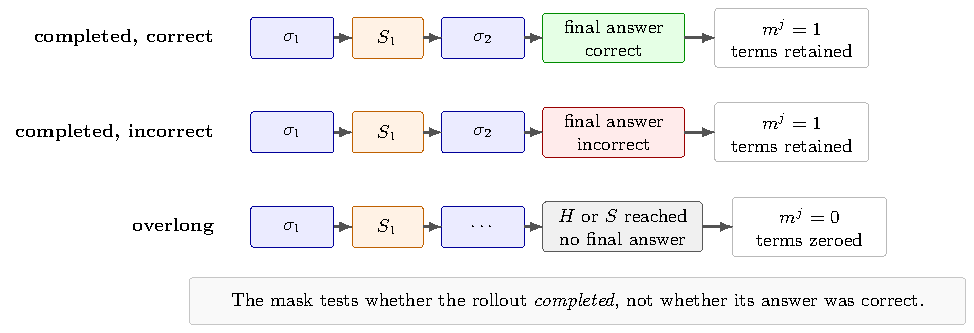
\includegraphics[width=0.98\linewidth]{figures/supo_overlong_mask.pdf}
    \caption{Effect of SUPO's overlong mask.  Both correct and incorrect
    completed rollouts contribute policy-gradient terms.  Only a rollout
    truncated by the step limit $H$ or summary limit $S$ before emitting a
    final answer has all of its token-level terms zeroed.}
    \label{fig:supo.overlong.mask}
\end{figure}

SUPO then maximizes the globally token-normalized objective
\begin{align}
    \Jcal_{\mathrm{SUPO}}(\theta)
    :=
    \frac{1}{\sum_{j=1}^{G}\lvert\Mcal^j\rvert}
    \sum_{j=1}^{G}
    \sum_{(t,\ell)\in\Mcal^j}
    m^j
    \min\left\{
        \rho_{t,\ell}^j(\theta)\widehat A^j,
        \operatorname{clip}\left(
            \rho_{t,\ell}^j(\theta),
            1-\epsilon_{\mathrm{low}},
            1+\epsilon_{\mathrm{high}}
        \right)\widehat A^j
    \right\}.
    \label{eq:supo.objective}
\end{align}
The mask removes the overlong rollout's own policy-gradient terms.  As written,
its reward can still affect the detached group mean and standard deviation in
Equation~\eqref{eq:supo.advantage}.  In the paper's ablation, removing the mask
causes summarization usage to collapse and reduces conditional success.  The
reported experiments use $G=8$, asymmetric clipping
$\epsilon_{\mathrm{low}}=0.20$ and
$\epsilon_{\mathrm{high}}=0.28$, and no KL or entropy penalty.

\paragraph{Comparison.}
The apparent tension between the papers is resolved by the unit at which the
advantage is computed.  CompactionRL avoids group-relative estimation and uses
a critic to give each token a temporally corrected advantage; it therefore
supports group size one.  SUPO remains critic-free by computing one relative
advantage per \emph{complete rollout before segmentation} and broadcasting it
to all of that rollout's tokens.  SUPO thereby handles the variable number of
subtrajectories without duplicating rewards in the group baseline, but it
cannot distinguish an early summary token from a late execution token within
the same rollout.  The compaction mechanism is shared; the principal
algorithmic difference is fine-grained temporal credit assignment versus a
coarser, critic-free group-relative baseline.
\input{agentic-rl/async-rl}

\chapter{Reward Modeling}
\section{Reward Modeling}
\label{sec:reward-modeling}

A reward model (RM) replaces a hand-written objective with a learned scoring function.  For a prompt $x$ and completion $y$, it estimates a scalar or a set
of local scores that can be used for best-of-$N$ selection, search, or policy optimization.  Unlike an environment reward, this signal is inferred from human preferences or correctness annotations and is therefore only a proxy for the desired behavior.

This section uses $x$ for a prompt, $y$ for a completion, $y_c$ for a chosen completion, and $y_r$ for a rejected completion.  It is adapted from Lambert's reward-modeling chapter.\footnote{
\url{https://rlhfbook.com/c/05-reward-models}}

\subsection{Bradley--Terry Preference Reward Model}

\subsubsection{Preference likelihood}

The Bradley--Terry (BT) model assigns each item $i$ a positive latent strength
$p_i$.  Its pairwise preference probability is
\begin{equation}
    P(i \succ j)
    =
    \frac{p_i}{p_i+p_j}.
\end{equation}
Writing $p_i=\exp(r_i)$ gives the logit parameterization
\begin{equation}
    P(i \succ j)
    =
    \frac{\exp(r_i)}{\exp(r_i)+\exp(r_j)}
    =
    \sigma(r_i-r_j),
    \qquad
    \sigma(z)=\frac{1}{1+\exp(-z)}.
\end{equation}
Consequently, only score differences are identifiable: replacing every score
$r_i$ by $r_i+C$ leaves all preference probabilities unchanged.

For an RM $r_\theta(x,y)$ and a preference triple
$(x,y_c,y_r)\sim\mathcal{D}$,
\begin{equation}
    P_\theta(y_c\succ y_r\mid x)
    =
    \sigma\!\left(
        r_\theta(x,y_c)-r_\theta(x,y_r)
    \right).
    \label{eq:bt-probability}
\end{equation}
Maximum likelihood yields the final loss function:
\begin{align}
    \mathcal{L}_{\mathrm{BT}}(\theta)
    &=
    \mathbb{E}_{(x,y_c,y_r)\sim\mathcal{D}}
    - \log \sigma\!\left(
        r_\theta(x,y_c)-r_\theta(x,y_r)
    \right).
    % &=
    % \mathbb{E}_{(x,y_c,y_r)\sim\mathcal{D}}
    % \operatorname{softplus}\!\left(
    %     r_\theta(x,y_r)-r_\theta(x,y_c)
    % \right).
    \label{eq:bt-loss}
\end{align}
The log is applied before averaging; maximizing
$\mathbb{E}[P_\theta(y_c\succ y_r\mid x)]$ is not the same likelihood
objective.

\subsubsection{Architecture}

The standard architecture reuses a causal-transformer backbone and replaces
its vocabulary projection with a scalar head.  For prompt-completion tokens
$z=(x,y)$, let $h_t\in\mathbb{R}^d$ be the final-layer hidden state.  A common
sequence score is
\begin{equation}
    r_\theta(x,y)=w^\top h_{t_{\mathrm{last}}}+b,
\end{equation}
where $t_{\mathrm{last}}$ is the final non-padding token, normally an EOS
token.  Chosen and rejected sequences are scored independently by the same
network.  The loss in \eqref{eq:bt-loss} couples only their scalar outputs.

\begin{codeblock}[language=Python,caption={Minimal Bradley--Terry reward model.}]
import torch
import torch.nn as nn
import torch.nn.functional as F

class BradleyTerryRM(nn.Module):
    def __init__(self, backbone):
        super().__init__()
        # Transformer producing one d-dimensional hidden state per token.
        self.backbone = backbone
        # Shared linear head: final token representation -> scalar reward.
        self.reward_head = nn.Linear(backbone.config.hidden_size, 1)

    def forward(self, input_ids, attention_mask):
        """
        Score each complete prompt-response sequence.

        input_ids:      token IDs, shape [batch_size, sequence_length]
        attention_mask: 1 for real tokens and 0 for padding, same shape
        returns:        one unnormalized reward logit per sequence, shape [B]
        """
        out = self.backbone(
            input_ids=input_ids,
            attention_mask=attention_mask,
            output_hidden_states=True,
            return_dict=True,
        )

        # Last transformer layer: one contextual representation per token.
        hidden = out.hidden_states[-1]              # [B, T, d]

        # Locate the final non-padding token. Unlike mask.sum() - 1, this is
        # correct for both left-padded and right-padded batches.
        positions = torch.arange(
            hidden.size(1), device=hidden.device
        ).expand_as(attention_mask)
        last = positions.masked_fill(attention_mask == 0, -1).max(dim=1).values
        batch = torch.arange(hidden.size(0), device=hidden.device)
        final_hidden = hidden[batch, last]           # [B, d], usually EOS

        # The score is not a probability; only score differences enter BT loss.
        return self.reward_head(final_hidden).squeeze(-1)  # [B]

def preference_loss(model, chosen, rejected):
    """Negative log-likelihood that chosen is preferred to rejected."""
    # Both dictionaries contain the same prompts but different completions.
    # The same reward model (shared parameters) scores both sequences.
    reward_chosen = model(**chosen)
    reward_rejected = model(**rejected)

    # -log sigmoid(r_chosen - r_rejected), averaged over the batch.
    # Minimization pushes the chosen score above the rejected score.
    return -F.logsigmoid(reward_chosen - reward_rejected).mean()
\end{codeblock}

Correct construction of the two inputs is critical: each contains the same
prompt and exactly one completion, and the attention mask must select the
actual final token under either left or right padding.  Reward models are
commonly trained for only one epoch because pairwise datasets are correlated
and overfitting can rapidly degrade held-out ranking accuracy.

\subsection{Outcome Reward Models}

An outcome reward model (ORM) predicts whether a completion eventually reaches
a correct final answer.  It is trained from independently labeled examples
$(x,y,r)$, where $r\in\{0,1\}$ denotes final-answer correctness; paired
chosen--rejected data is unnecessary.

One common ORM emits a binary logit $w_{\theta,t}$ at every completion token.
The sequence outcome label is broadcast across completion positions while
prompt and padding positions are masked:
\begin{equation}
    \mathcal{L}_{\mathrm{ORM}}(\theta)
    =
    -\mathbb{E}_{(x,y,r)\sim\mathcal{D}}
    \left[
        \frac{1}{\sum_t m_t}
        \sum_{t=1}^{T}m_t
        \left(
            r\log p_{\theta,t}
            +(1-r)\log(1-p_{\theta,t})
        \right)
    \right],
    \label{eq:orm-token-loss}
\end{equation}
where $m_t=1$ only for completion tokens and
$p_{\theta,t}=\sigma(w_{\theta,t})$.  These targets contain no direct
information about whether an intermediate step is valid: every token receives
the label determined by the final outcome.

A sequence-pooled alternative first averages logits and then applies the
sigmoid,
\begin{equation}
    \bar p_\theta(x,y)
    =
    \sigma\!\left(
        \frac{1}{\sum_t m_t}\sum_t m_t w_{\theta,t}
    \right),
\end{equation}
followed by sequence-level binary cross entropy.  In general,
$\sigma(\operatorname{mean}(w_t))\neq
\operatorname{mean}(\sigma(w_t))$, so these aggregation orders are not
interchangeable.

\begin{codeblock}[language=Python,caption={Per-token outcome reward model.}]
import torch.nn as nn
import torch.nn.functional as F

class OutcomeRM(nn.Module):
    def __init__(self, backbone):
        super().__init__()
        self.backbone = backbone
        self.outcome_head = nn.Linear(backbone.config.hidden_size, 1)

    def forward(self, input_ids, attention_mask, labels=None):
        out = self.backbone(
            input_ids=input_ids,
            attention_mask=attention_mask,
            output_hidden_states=True,
            return_dict=True,
        )
        hidden = out.hidden_states[-1]
        logits = self.outcome_head(hidden).squeeze(-1)  # [B, T]

        if labels is None:
            return {"logits": logits}

        # labels: -100 for prompt/padding; 0 or 1 for completion tokens
        mask = labels.ne(-100)
        loss = F.binary_cross_entropy_with_logits(
            logits[mask], labels[mask].float()
        )
        return {"loss": loss, "logits": logits}
\end{codeblock}

At inference, the per-token probabilities can be reduced to a candidate score
using the mean, the last few positions, the minimum, or a sum of log
probabilities.  The reduction must match validation-time behavior; products
strongly penalize long completions and minimum aggregation is highly sensitive
to one anomalous token.

\subsection{Process Reward Models}

A process reward model (PRM) evaluates intermediate reasoning steps rather than
only the final answer.  Let
$s=(s_1,\ldots,s_K)$ be an annotated reasoning trace and let
$q_i\in\{0,1\}$ indicate whether step $s_i$ is valid conditioned on the prompt
and previous steps.  A binary PRM minimizes
\begin{equation}
    \mathcal{L}_{\mathrm{PRM}}(\theta)
    =
    -\mathbb{E}_{(x,s)\sim\mathcal{D}}
    \sum_{i=1}^{K}
    \left[
        q_i\log r_\theta(s_i\mid x,s_{<i})
        +(1-q_i)\log\!\left(1-r_\theta(s_i\mid x,s_{<i})\right)
    \right].
    \label{eq:prm-loss}
\end{equation}
In practice, a separator token marks each step boundary.  All non-boundary
positions receive the ignore index $-100$.  A common three-class formulation
uses class indices $0,1,2$ for incorrect, neutral, and correct.

\begin{codeblock}[language=Python,caption={Three-class process reward model.}]
import torch.nn as nn
import torch.nn.functional as F

class ProcessRM(nn.Module):
    def __init__(self, backbone, num_classes=3):
        super().__init__()
        self.backbone = backbone
        self.step_head = nn.Linear(
            backbone.config.hidden_size, num_classes
        )

    def forward(self, input_ids, attention_mask, labels=None):
        out = self.backbone(
            input_ids=input_ids,
            attention_mask=attention_mask,
            output_hidden_states=True,
            return_dict=True,
        )
        logits = self.step_head(out.hidden_states[-1])  # [B, T, 3]

        if labels is None:
            return {"logits": logits}

        # labels: 0=incorrect, 1=neutral, 2=correct at boundaries;
        #         -100 at every other token.
        loss = F.cross_entropy(
            logits.reshape(-1, logits.size(-1)),
            labels.reshape(-1),
            ignore_index=-100,
        )
        return {"loss": loss, "logits": logits}
\end{codeblock}

For search or reranking, PRM outputs are read only at step boundaries.  Step
scores can be averaged, summed with position-dependent weights, or reduced by
the minimum to reject a trace as soon as one step is judged invalid.

\subsection{Reward Models versus Value Functions}

The output shape alone does not define the model.  The supervision target and
its semantics are decisive:

\begin{center}
\small
\begin{tabularx}{\textwidth}{@{}l X X l@{}}
\toprule
Model & Prediction & Supervision & Output location \\
\midrule
BT RM
& Relative quality $r_\theta(x,y)$
& Pairwise preferences
& EOS/last token \\
ORM
& Probability of eventual correctness
& Fixed offline outcome label
& Every completion token \\
PRM
& Validity of the current reasoning step
& Step-level annotations
& Step boundaries \\
Value function
& Expected remaining return $V^\pi(s_t)$
& Return targets from policy rollouts
& Every policy token \\
\bottomrule
\end{tabularx}
\end{center}

A value function predicts
\begin{equation}
    V^\pi(s_t)
    =
    \mathbb{E}_{\pi}\!\left[
        \sum_{k=t}^{T}\gamma^{k-t}r_k
        \,\middle|\,s_t
    \right].
\end{equation}
Its targets generally depend on the current policy's rollouts and change as
that policy changes.  By contrast, an ORM is normally trained offline against
fixed correctness labels broadcast to token prefixes.  Even if both use the
same backbone and scalar per-token head, the ORM estimates outcome
correctness, whereas the value head estimates remaining return and serves as a
baseline for advantages such as
$A_t=\widehat{R}_t-V_\phi(s_t)$.

Training a sequence-level BT model on pairs formed by one correct and one
incorrect response does \emph{not} turn it into an ORM.  If the objective is
\eqref{eq:bt-loss} and the output is one scalar per sequence, it remains a
pairwise preference RM; correctness merely determines how the pairs were
constructed.

\subsection{Inference Interfaces}

\begin{description}
    \item[BT RM.]
    Input $(x,y)$; output one scalar $r_\theta(x,y)$.  Use it as a terminal
    RL reward or rank $N$ sampled completions by their scalar scores.

    \item[ORM.]
    Input $(x,y)$; output
    $p_t\approx P(\text{final answer correct}\mid x,y_{\leq t})$ at completion
    positions.  Aggregate token scores to verify or rerank finished
    candidates.

    \item[PRM.]
    Input $(x,s_1,\ldots,s_K)$; output correctness scores at step boundaries.
    Aggregate across steps for reranking, or use scores online to prune
    low-quality search branches.

    \item[Value function.]
    Input the current prefix state $s_t=(x,y_{<t})$; output $V_\phi(s_t)$.
    During RL training it provides a per-token baseline rather than an
    interpretable probability that the whole response is correct.
\end{description}


\chapter{Distillation}

\textbf{Off-policy distillation} trains the student on sequences generated by
another source, such as human-annotated data or outputs produced in advance by
a teacher model. Classical knowledge distillation is typically off-policy: the student learns to match
the teacher's output distribution on teacher-generated trajectories.
Informally, the student learns from model answers written by others.

\textbf{On-policy distillation} instead uses trajectories sampled online from
the student's current policy. The teacher provides token-level supervision on
these student-generated trajectories. After each student update, new
trajectories are sampled from the updated policy. In this setting, the student
produces its own answers, and the teacher evaluates how it should proceed.
 
This distinction is important because it affects \textbf{exposure bias}.
Under off-policy distillation, the student is trained primarily on high-quality
teacher or reference trajectories. During inference, however, it conditions
on its own outputs. An early mistake may move the student into a state rarely
represented in the training data, causing subsequent errors to accumulate.
Exposure bias thus arises partly from the mismatch between the
teacher/reference distribution observed during training and the
student-induced state distribution encountered during generation.

On-policy training reduces this mismatch by training on trajectories produced
by the current student policy. Even erroneous states encountered during
rollout become training examples, allowing the teacher to provide supervision
at states the student is likely to visit. This better aligns the training and
inference distributions, thereby mitigating exposure bias and compounding
errors.

On-policy training does not, however, eliminate exposure bias entirely.
Differences in teacher and student capabilities, low-quality rollouts,
distributional drift over long sequences, and optimization instability may
still create discrepancies between training and inference. More precisely,
on-policy distillation mitigates exposure bias at the data-distribution level
rather than removing it at its source. Its central advantage over purely
off-policy distillation is that the student learns not only what the teacher
would do along ideal trajectories, but also what the teacher recommends in
states reached by the student itself.

\begin{figure}[!ht]
    \centering
    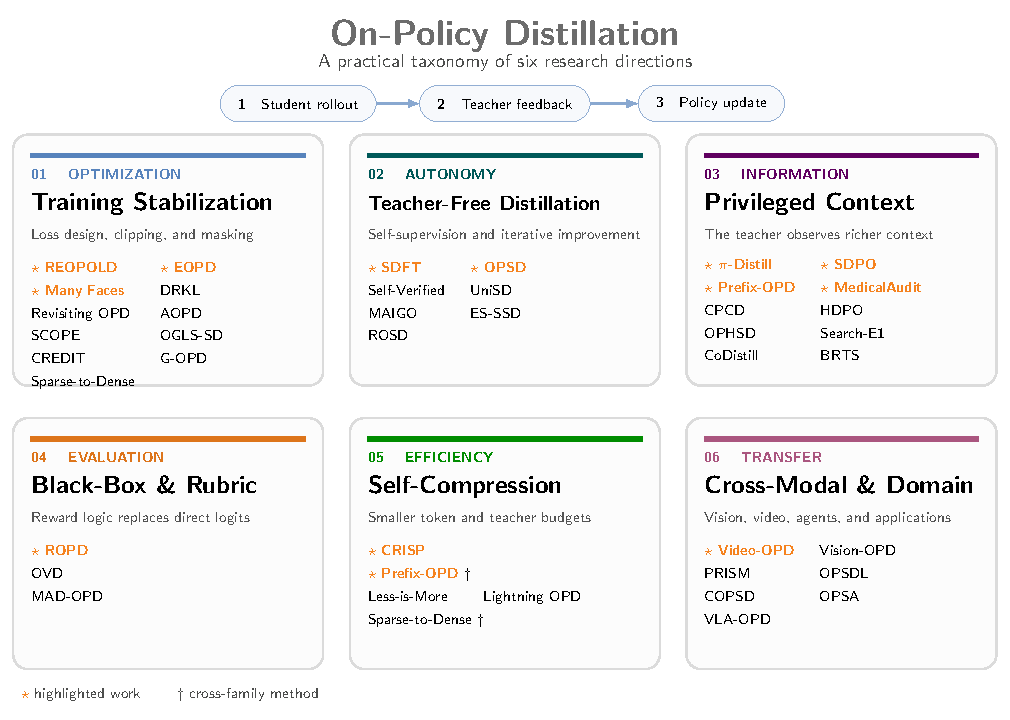
\includegraphics[width=\linewidth]{figures/opd_taxonomy.pdf}
    \caption{Six research directions in on-policy distillation, organized by the
    main source of innovation.}
    \label{fig:opd-taxonomy}
\end{figure}

\clearpage
\section{On-Policy Distillation: Basics}
\label{sec:on-policy-distillation-basics}

On-policy distillation (OPD) computes supervision on trajectories sampled from
the current student policy $\pi_\theta$. Given a prompt $x\sim\Dcal_x$, the
student samples a response
\begin{align*}
    y &\sim \pi_\theta(\cdot\mid x),
    \qquad T(y) \coloneqq |y| \text{ (the length of the response)},\\
    y &= (y_1,\ldots,y_{T(y)}),
\end{align*}
where the end-of-sequence token is included in the response. Both the student
and the fixed teacher $\pi_{\mathrm{Teacher}}$ are evaluated on each
student-generated prefix $y_{<t}$. Their next-token distributions are, for all $v\in\Vcal$ (the vocabulary),
\begin{align*}
    p_t(v)
    \coloneqq \pi_\theta(v\mid x,y_{<t}),
    \quad\text{and}\quad
    q_t(v)
    \coloneqq \pi_{\mathrm{Teacher}}(v\mid x,y_{<t}).
\end{align*}

A standard formulation minimizes the sequence-level reverse KL on the prompt
distribution. Let $\Ycal(x)$ denote the set of complete responses to $x$, and
define the joint distribution $\mu_\theta$ by sampling
$x\sim\Dcal_x$ first and then $y\sim\pi_\theta(\cdot\mid x)$. In the discrete
case, this means
$\mu_\theta(x,y)=\Dcal_x(x)\pi_\theta(y\mid x)$. Expanding the KL before
combining the expectations gives
\begin{align}
    \Lcal_{\mathrm{OPD}}(\theta)
    &=
    \E_{x\sim\Dcal_x}
    \left[
        D_{\mathrm{KL}}\!\left(
            \pi_\theta(\cdot\mid x)
            \,\middle\|\,
            \pi_{\mathrm{Teacher}}(\cdot\mid x)
        \right)
    \right]
    \nonumber\\
    &=
    \E_{x\sim\Dcal_x}
    \left[
        \sum_{y\in\Ycal(x)}
        \pi_\theta(y\mid x)
        \log\frac{\pi_\theta(y\mid x)}
                 {\pi_{\mathrm{Teacher}}(y\mid x)}
    \right]
    \nonumber\\
    &=
    \E_{x\sim\Dcal_x}
    \left[
        \E_{y\sim\pi_\theta(\cdot\mid x)}
        \left[
            \log\frac{\pi_\theta(y\mid x)}
                     {\pi_{\mathrm{Teacher}}(y\mid x)}
        \right]
    \right]
    \nonumber\\
    &=
    \E_{(x,y)\sim\mu_\theta}
    \left[
        \log\frac{\pi_\theta(y\mid x)}
                 {\pi_{\mathrm{Teacher}}(y\mid x)}
    \right].
    \label{eq:opd.sequence-kl}
\end{align}
The last line is the law of total expectation. It does not make $x$ and $y$
independent: their joint law is $\mu_\theta$, under which the response $y$ is
conditioned on the sampled prompt $x$.

\begin{highlight}
    \eqref{eq:opd.sequence-kl} can be equivalently rewritten as the token-level form loss function
    \begin{align*}
        \Lcal_{\mathrm{OPD}}(\theta)
        =
        \E_{(x,y)\sim\mu_\theta}
        \left[
            \sum_{t=1}^{T(y)}
            D_{\mathrm{KL}}\!\left(
                \pi_\theta(\cdot\mid x,y_{<t})
                \,\middle\|\,
                \pi_{\mathrm{Teacher}}(\cdot\mid x,y_{<t})
            \right)
        \right].
    \end{align*}
\end{highlight}

To obtain the token-level form, fix a prompt $x$ and abbreviate the student
and teacher sequence probabilities by $P_\theta(y\mid x)$ and
$Q_{\mathrm{Teacher}}(y\mid x)$. Autoregressive factorization gives
\begin{align}
    P_\theta(y\mid x)
    &=
    \prod_{t=1}^{T(y)}\pi_\theta(y_t\mid x,y_{<t}),
    &
    Q_{\mathrm{Teacher}}(y\mid x)
    &=
    \prod_{t=1}^{T(y)}
    \pi_{\mathrm{Teacher}}(y_t\mid x,y_{<t}).
    \label{eq:opd.factorization}
\end{align}
Substituting these products into the definition of KL and using
$\log\prod_t a_t=\sum_t\log a_t$ yields
\begin{align}
    &D_{\mathrm{KL}}\!\left(
        P_\theta(\cdot\mid x)
        \,\middle\|\,
        Q_{\mathrm{Teacher}}(\cdot\mid x)
    \right)
    \nonumber\\
    &\quad=
    \sum_y P_\theta(y\mid x)
    \log\frac{P_\theta(y\mid x)}{Q_{\mathrm{Teacher}}(y\mid x)}
    = 
    \E_{y\sim\pi_\theta(\cdot\mid x)}
    \left[
        \log
        \frac{
            \prod_{t=1}^{T(y)}\pi_\theta(y_t\mid x,y_{<t})
        }{
            \prod_{t=1}^{T(y)}
            \pi_{\mathrm{Teacher}}(y_t\mid x,y_{<t})
        }
    \right]
    \nonumber\\
    &\quad=
    \E_{y\sim\pi_\theta(\cdot\mid x)}
    \left[
        \sum_{t=1}^{T(y)}
        \log
        \frac{
            \pi_\theta(y_t\mid x,y_{<t})
        }{
            \pi_{\mathrm{Teacher}}(y_t\mid x,y_{<t})
        }
    \right].
    \label{eq:opd.log-ratio-sum}
\end{align}
For a fixed $x$ and a realized prefix $y_{<t}$, define the corresponding conditional reverse KL by
\begin{align}
    \mathrm{kl}_t(x,y_{<t})
    &\coloneqq
    \E_{v\sim\pi_\theta(\cdot\mid x,y_{<t})}
    \left[\log\frac{\pi_\theta(v\mid x,y_{<t})}{\pi_{\mathrm{Teacher}}(v\mid x,y_{<t})}\right]
    \nonumber\\
    &=
    D_{\mathrm{KL}}\!\left(
        \pi_\theta(\cdot\mid x,y_{<t})
        \,\middle\|\,
        \pi_{\mathrm{Teacher}}(\cdot\mid x,y_{<t})
    \right).
    \label{eq:opd.conditional-token-kl}
\end{align}

Assume that generation is capped at $T_{\max}$. For each $t$, the indicator
$\mathbf{1}\{t\leq T(y)\}$ is determined by $y_{<t}$ because it only records
whether an end-of-sequence token has already appeared. Therefore it can be
pulled through the conditional expectation over the next token. Using the
tower property term by term gives
\begin{align}
    &\E_{y\sim\pi_\theta(\cdot\mid x)}
    \left[
        \sum_{t=1}^{T(y)}
        \log\frac{\pi_\theta(y_t\mid x,y_{<t})}{\pi_{\mathrm{Teacher}}(y_t\mid x,y_{<t})}
    \right]
    \nonumber\\
    &\quad=
    \sum_{t=1}^{T_{\max}}
    \E_{y\sim\pi_\theta(\cdot\mid x)}
    \left[
        \mathbf{1}\{t\leq T(y)\}
        \log\frac{\pi_\theta(y_t\mid x,y_{<t})}{\pi_{\mathrm{Teacher}}(y_t\mid x,y_{<t})}
    \right]
    \nonumber\\
    &\quad=
    \sum_{t=1}^{T_{\max}}
    \E_{y\sim\pi_\theta(\cdot\mid x)}
    \left[
        \mathbf{1}\{t\leq T(y)\}
        \E_{v\sim\pi_\theta(\cdot\mid x,y_{<t})}
        \left[\log\frac{\pi_\theta(v\mid x,y_{<t})}{\pi_{\mathrm{Teacher}}(v\mid x,y_{<t})}\right]
    \right]
    \nonumber\\
    &\quad=
    \E_{y\sim\pi_\theta(\cdot\mid x)}
    \left[
        \sum_{t=1}^{T(y)}
        \mathrm{kl}_t(x,y_{<t})
    \right].
    \label{eq:opd.tower-decomposition}
\end{align}
The second equality follows by conditioning each outer expectation on the
realized prefix $y_{<t}$. Conditional on $x$ and $y_{<t}$, the actual next
token has distribution
$y_t\sim\pi_\theta(\cdot\mid x,y_{<t})$. Its conditional mean is therefore
$\E_{v\sim\pi_\theta(\cdot\mid x,y_{<t})} \left[\log\frac{\pi_\theta(v\mid x,y_{<t})}{\pi_{\mathrm{Teacher}}(v\mid x,y_{<t})}\right]$, where $v$ is only a dummy variable for the next token and the resulting quantity depends only on $y_{<t}$;
averaging it under the complete-response distribution $y\sim
\pi_\theta(\cdot\mid x)$ simply averages over the student-induced prefixes.
The unobserved suffix integrates to one.

Combining \eqref{eq:opd.log-ratio-sum},
\eqref{eq:opd.conditional-token-kl}, and
\eqref{eq:opd.tower-decomposition}, then restoring the prompt expectation,
yields
\begin{align}
    \Lcal_{\mathrm{OPD}}(\theta)
    =
    \E_{(x,y)\sim\mu_\theta}
    \left[
        \sum_{t=1}^{T(y)}
        D_{\mathrm{KL}}\!\left(
            \pi_\theta(\cdot\mid x,y_{<t})
            \,\middle\|\,
            \pi_{\mathrm{Teacher}}(\cdot\mid x,y_{<t})
        \right)
    \right].
    \label{eq:opd.token-kl}
\end{align}

\subsection{Implemnted OPD Objectives}
In practice, the actual loss computation varies with different implementations on how this exact per-token reverse KL is computed. We will see some examples below.

\begin{itemize}
    \item \textbf{Sampled-token OPD.}
    The lightest variant evaluates the log-ratio only at the token $y_t$
    sampled by the student. At a realized prefix $(x,y_{<t})$, define
    \begin{align}
        \ell_t^{\mathrm{sample}}(x,y_{\leq t})
        \coloneqq
        \log p_t(y_t)-\log q_t(y_t).
        \label{eq:opd.sampled-token-loss}
    \end{align}
    Its token-level objective is
    \begin{highlight}
        \begin{align}
            \Lcal_{\mathrm{OPD}}^{\mathrm{sample}}(\theta)
            =
            \E_{(x,y)\sim\mu_\theta}
            \left[
                \sum_{t=1}^{T(y)}
                \ell_t^{\mathrm{sample}}(x,y_{\leq t})
            \right].
            \label{eq:opd.sampled-token-objective}
        \end{align}
    \end{highlight}
    Since $y_t\sim p_t$ conditional on $(x,y_{<t})$,
    \begin{align}
        \E_{y_t\sim p_t}
        \left[
            \ell_t^{\mathrm{sample}}(x,y_{\leq t})
        \right]
        =
        \sum_{v\in\Vcal}p_t(v)\log\frac{p_t(v)}{q_t(v)}
        =
        D_{\mathrm{KL}}(p_t\|q_t).
        \label{eq:opd.sampled-token-unbiased}
    \end{align}
    Thus, the sampled-token loss is an unbiased one-sample estimator of the
    scalar token-level reverse KL at the sampled prefix.

    \item \textbf{Full-vocabulary OPD.}
    This variant evaluates the divergence over the entire vocabulary at every
    sampled prefix:
    \begin{highlight}
        \begin{align}
            \Lcal_{\mathrm{OPD}}^{\mathrm{full}}(\theta)
            =
            \E_{(x,y)\sim\mu_\theta}
            \left[
                \sum_{t=1}^{T(y)}
                D_{\mathrm{KL}}(p_t\|q_t)
            \right].
            \label{eq:opd.full-vocabulary-objective}
        \end{align}
    \end{highlight}
    It provides dense supervision but materializing both distributions costs
    $O(BT_{\max}\Vcal)$ ( where $|\Vcal|$ is the vocabulary size) memory for batch size $B$.

    \item \textbf{Student-top-$k$ OPD.}
    This intermediate variant restricts the divergence to the $k$ tokens with
    highest student probability:
    \begin{align*}
        S_t\coloneqq S_t(x,y_{<t})
        \coloneqq
        \operatorname{TopK}(p_t,k)
        \subseteq \Vcal.
    \end{align*}
    Both distributions are renormalized on this same support:
    \begin{align}
        \bar p_t^{(S_t)}(v)
        &\coloneqq
        \frac{p_t(v)\mathbf{1}\{v\in S_t\}}
             {\sum_{u\in S_t}p_t(u)},
        &
        \bar q_t^{(S_t)}(v)
        &\coloneqq
        \frac{q_t(v)\mathbf{1}\{v\in S_t\}}
             {\sum_{u\in S_t}q_t(u)}.
        \label{eq:opd.top-k-renormalization}
    \end{align}
    The resulting objective is
    \begin{highlight}
        \begin{align}
            \Lcal_{\mathrm{OPD}}^{\mathrm{top}\text{-}k}(\theta)
            =
            \E_{(x,y)\sim\mu_\theta}
            \left[
                \sum_{t=1}^{T(y)}
                D_{\mathrm{KL}}\!\left(
                    \bar p_t^{(S_t)}
                    \,\middle\|\,
                    \bar q_t^{(S_t)}
                \right)
            \right].
            \label{eq:opd.top-k-objective}
        \end{align}
    \end{highlight}

    \begin{remark}
        \item
        \begin{itemize}
        \item Probability mass outside $S_t$ is discarded, so this is generally not
        equal to the full-vocabulary reverse KL. It preserves multi-token
        supervision on the student's high-probability region at lower cost. In other words, the sampled-token OPD is unbiased yet suffers from high variance while the full-vocabulary OPD is unbiased and has lower variance, yet it requires more memory. Top-k OPD is a compromise between the two, it is biased but has lower variance than sampled-token OPD. It also loses the probability mass information outside $S_t$.

        \item \textbf{\eqref{eq:opd.top-k-objective} is ill-defined when $k=1$.} When $k=1$, this objective seems to degenerate. If $S_t = \{v^*_t\}$, then both restricted distributions become point masses after renormalization $\bar p_t(v^*_t) = 1, \bar q_t(v^*_t) = 1$, so the KL is identically zero. This would provide no distillation signal.
        
        \item    \textbf{When is top-$k$ OPD a good surrogate for full-vocabulary OPD?}
        Define the mass each distribution places on the student top-$k$ set,
        $P_{S_t}=\sum_{v\in S_t}p_t(v)$ and $Q_{S_t}=\sum_{v\in S_t}q_t(v)$.
        Write $S_t^c=\Vcal\setminus S_t$ for the complement, and assume
        $0<P_{S_t},Q_{S_t}<1$ so that both pieces below are proper distributions.
        Renormalize on the complement in the same way as
        \eqref{eq:opd.top-k-renormalization}:
        \begin{align}
            p_t^{S_t^c}(v)
            &\coloneqq
            \frac{p_t(v)\mathbf{1}\{v\in S_t^c\}}{1-P_{S_t}},
            &
            q_t^{S_t^c}(v)
            &\coloneqq
            \frac{q_t(v)\mathbf{1}\{v\in S_t^c\}}{1-Q_{S_t}}.
            \label{eq:opd.complement-renormalization}
        \end{align}
        Partition the reverse KL into the top-$k$ support and its complement:
        \begin{align}
            D_{\mathrm{KL}}(p_t\|q_t)
            &=
            \sum_{v\in\Vcal}p_t(v)\log\frac{p_t(v)}{q_t(v)}
            \nonumber\\
            &=
            \sum_{v\in S_t}p_t(v)\log\frac{p_t(v)}{q_t(v)}
            +
            \sum_{v\in S_t^c}p_t(v)\log\frac{p_t(v)}{q_t(v)}.
            \label{eq:opd.kl-split}
        \end{align}
        On $S_t$, the renormalization
        \eqref{eq:opd.top-k-renormalization} says
        $p_t(v)=P_{S_t}\bar p_t^{(S_t)}(v)$ and
        $q_t(v)=Q_{S_t}\bar q_t^{(S_t)}(v)$. Substituting and using
        $\sum_{v\in S_t}\bar p_t^{(S_t)}(v)=1$ separates the shape of the
        conditional distribution from the mass on the set:
        \begin{align}
            \sum_{v\in S_t}p_t(v)\log\frac{p_t(v)}{q_t(v)}
            &=
            \sum_{v\in S_t}
            P_{S_t}\bar p_t^{(S_t)}(v)
            \log\frac{P_{S_t}\bar p_t^{(S_t)}(v)}{Q_{S_t}\bar q_t^{(S_t)}(v)}
            \nonumber\\
            &=
            P_{S_t}
            \sum_{v\in S_t}
            \bar p_t^{(S_t)}(v)
            \left(
                \log\frac{\bar p_t^{(S_t)}(v)}{\bar q_t^{(S_t)}(v)}
                +
                \log\frac{P_{S_t}}{Q_{S_t}}
            \right)
            \nonumber\\
            &=
            P_{S_t}\,
            D_{\mathrm{KL}}\!\left(
                \bar p_t^{(S_t)}
                \,\middle\|\,
                \bar q_t^{(S_t)}
            \right)
            +
            P_{S_t}\log\frac{P_{S_t}}{Q_{S_t}}.
            \label{eq:opd.kl-on-support}
        \end{align}
        The same substitution on the complement,
        $p_t(v)=(1-P_{S_t})p_t^{S_t^c}(v)$ and
        $q_t(v)=(1-Q_{S_t})q_t^{S_t^c}(v)$, gives
        \begin{align}
            \sum_{v\in S_t^c}p_t(v)\log\frac{p_t(v)}{q_t(v)}
            &=
            (1-P_{S_t})\,
            D_{\mathrm{KL}}\!\left(
                p_t^{S_t^c}
                \,\middle\|\,
                q_t^{S_t^c}
            \right)
            +
            (1-P_{S_t})\log\frac{1-P_{S_t}}{1-Q_{S_t}}.
            \label{eq:opd.kl-on-complement}
        \end{align}
        The two scalar terms are the KL between Bernoulli random variables that
        only record whether the next token falls in $S_t$. If
        $Z\sim\mathrm{Bern}(P_{S_t})$ and $W\sim\mathrm{Bern}(Q_{S_t})$, then
        \begin{align}
            D_{\mathrm{KL}}(Z\|W)
            &=
            P_{S_t}\log\frac{P_{S_t}}{Q_{S_t}}
            +
            (1-P_{S_t})\log\frac{1-P_{S_t}}{1-Q_{S_t}}.
            \label{eq:opd.bernoulli-kl}
        \end{align}
        Adding \eqref{eq:opd.kl-on-support} and \eqref{eq:opd.kl-on-complement},
        and identifying \eqref{eq:opd.bernoulli-kl}, produces the decomposition
        \begin{align}
            D_{\mathrm{KL}}(p_t\|q_t)
            &=
            P_{S_t}\,
            D_{\mathrm{KL}}\!\left(
                \bar p_t^{(S_t)}
                \,\middle\|\,
                \bar q_t^{(S_t)}
            \right)
            +
            (1-P_{S_t})\,
            D_{\mathrm{KL}}\!\left(
                p_t^{S_t^c}
                \,\middle\|\,
                q_t^{S_t^c}
            \right)
            \nonumber\\
            &\quad+
            D_{\mathrm{KL}}\!\left(
                \mathrm{Bern}(P_{S_t})
                \,\middle\|\,
                \mathrm{Bern}(Q_{S_t})
            \right).
            \label{eq:opd.kl-decomposition}
        \end{align}
        Top-$k$ OPD keeps only the renormalized divergence on $S_t$, and it
        drops the weight $P_{S_t}$. The other two terms are the bias. The
        complement term vanishes as $P_{S_t}\to 1$, which is the regime in which
        the student's top-$k$ set already carries essentially all of its mass.
        The Bernoulli term is small when $P_{S_t}\approx Q_{S_t}$, i.e., when
        the teacher places a similar fraction of its mass on that same set. In
        that regime $P_{S_t}\approx 1$ as well, so dropping the weight changes
        the objective by little. Outside it, top-$k$ OPD ignores both how the
        leftover mass is shaped and how much total mass each model assigns to
        $S_t$.
        \end{itemize}
    \end{remark}
\end{itemize}

\subsection{Gradients of the OPD Objective}
\label{sec:opd.gradients}

The three variants above describe what is \emph{computed}; this section describes what
is \emph{differentiated}. We first derive the exact gradient of
\eqref{eq:opd.token-kl}, then show that standard OPD keeps only part of it, and finally
check, variant by variant, whether plain backpropagation produces that part.

Throughout, the teacher is fixed, so $\nabla_\theta q_t=0$. We use one identity
repeatedly: for any probability $\pi_\theta(z)>0$ that is differentiable in $\theta$,
the chain rule gives
\begin{align}
    \pi_\theta(z)\,\nabla_\theta\log\pi_\theta(z)
    =
    \pi_\theta(z)\,\frac{\nabla_\theta\pi_\theta(z)}{\pi_\theta(z)}
    =
    \nabla_\theta\pi_\theta(z).
    \label{eq:opd.log-derivative}
\end{align}
We also use the stop-gradient operator $\operatorname{sg}[\cdot]$ (\texttt{.detach()} in code), with
the following convention. $\operatorname{sg}$ appears only inside an expression that is still to
be differentiated, i.e., a loss, a surrogate, or an advantage that enters a loss, where it marks a
factor that is treated as a constant under $\nabla_\theta$. An expression that already contains
$\nabla_\theta$ never carries $\operatorname{sg}$: every factor outside $\nabla_\theta$ is simply a
value at the current $\theta$.

\paragraph{The exact gradient.}
In \eqref{eq:opd.token-kl}, $\theta$ enters in two places: inside each per-state KL loss
$\mathrm{kl}_t(x,y_{<t})$ defined in \eqref{eq:opd.conditional-token-kl}, through $\pi_\theta(\cdot\mid x,y_{<t})$, and through $\mu_\theta$, which determines which prefixes $y_{<t}$ are visited. The prompt
distribution $\Dcal_x$ does not depend on $\theta$, so fix $x$ and differentiate
\begin{align*}
    J_x(\theta)
    & \coloneqq
    \E_{y\sim\pi_\theta(\cdot\mid x)}
    \left[
        \sum_{t=1}^{T(y)}
    D_{\mathrm{KL}}\!\left(
        \pi_\theta(\cdot\mid x,y_{<t})
        \,\middle\|\,
        \pi_{\mathrm{Teacher}}(\cdot\mid x,y_{<t})\right)
    \right].
    \nonumber\\
    & =
    \E_{y\sim\pi_\theta(\cdot\mid x)}
    \left[
        \sum_{t=1}^{T(y)}\mathrm{kl}_t(x,y_{<t})
    \right].
\end{align*}
\begin{enumerate}
    \item \emph{Reduce each term to a sum over prefixes.} As in the derivation of
    \eqref{eq:opd.tower-decomposition}, cap generation at $T_{\max}$ and use the indicator
    $\mathbf{1}\{t\leq T(y)\}$, which is determined by $y_{<t}$. The $t$-th summand then
    depends on $y$ only through $y_{<t}$, so its expectation only needs the marginal
    probability of the prefix,
    $\pi_\theta(y_{<t}\mid x)=\prod_{s=1}^{t-1}p_s(y_s)$:
    \begin{align*}
        J_x(\theta)
        =
        \sum_{t=1}^{T_{\max}}
        \sum_{y_{<t}}
        \pi_\theta(y_{<t}\mid x)\,
        \mathbf{1}\{t\leq T(y)\}\,
        \mathrm{kl}_t(x,y_{<t}).
    \end{align*}
    \item \emph{Product rule.} Every sum is finite, so the gradient passes inside. Each
    summand is a product of two $\theta$-dependent factors, $\pi_\theta(y_{<t}\mid x)$ and
    $\mathrm{kl}_t(x,y_{<t})$; the indicator does not depend on $\theta$. Applying the
    product rule, then \eqref{eq:opd.log-derivative} to $\nabla_\theta\pi_\theta(y_{<t}\mid x)$,
    \begin{align*}
        \nabla_\theta J_x(\theta)
        &=
        \sum_{t=1}^{T_{\max}}
        \sum_{y_{<t}}
        \mathbf{1}\{t\leq T(y)\}
        \left[
            \pi_\theta(y_{<t}\mid x)\,\nabla_\theta\mathrm{kl}_t(x,y_{<t})
            +
            \mathrm{kl}_t(x,y_{<t})\,\nabla_\theta\pi_\theta(y_{<t}\mid x)
        \right]
        \\
        &=
        \sum_{t=1}^{T_{\max}}
        \sum_{y_{<t}}
        \pi_\theta(y_{<t}\mid x)\,
        \mathbf{1}\{t\leq T(y)\}
        \left[
            \nabla_\theta\mathrm{kl}_t(x,y_{<t})
            +
            \mathrm{kl}_t(x,y_{<t})\,\nabla_\theta\log\pi_\theta(y_{<t}\mid x)
        \right].
    \end{align*}
    Undoing step 1 (the bracket still depends on $y$ only through $y_{<t}$) turns this
    back into an expectation over complete responses:
    \begin{align*}
        \nabla_\theta J_x(\theta)
        =
        \E_{y\sim\pi_\theta(\cdot\mid x)}
        \left[
            \sum_{t=1}^{T(y)}\nabla_\theta\mathrm{kl}_t(x,y_{<t})
        \right]
        +
        \E_{y\sim\pi_\theta(\cdot\mid x)}
        \left[
            \sum_{t=1}^{T(y)}\mathrm{kl}_t(x,y_{<t})\,\nabla_\theta\log\pi_\theta(y_{<t}\mid x)
        \right].
    \end{align*}
    \item \emph{Expand the prefix score.} Taking the log of
    $\pi_\theta(y_{<t}\mid x)=\prod_{s=1}^{t-1}p_s(y_s)$ gives
    $\nabla_\theta\log\pi_\theta(y_{<t}\mid x)=\sum_{s=1}^{t-1}\nabla_\theta\log p_s(y_s)$.
    The second expectation therefore contains the double sum
    \begin{align*}
        \sum_{t=1}^{T(y)}\sum_{s=1}^{t-1}
        \mathrm{kl}_t(x,y_{<t})\,\nabla_\theta\log p_s(y_s).
    \end{align*}
    \item \emph{Swap the order of summation.} The double sum runs over all pairs
    $1\leq s<t\leq T(y)$. Summing over $s$ on the outside instead,
    \begin{align*}
        \sum_{t=1}^{T(y)}\sum_{s=1}^{t-1}
        \mathrm{kl}_t(x,y_{<t})\,\nabla_\theta\log p_s(y_s)
        =
        \sum_{s=1}^{T(y)}
        \nabla_\theta\log p_s(y_s)
        \sum_{t=s+1}^{T(y)}\mathrm{kl}_t(x,y_{<t}).
    \end{align*}
    Renaming $s\to t$ and $t\to t'$ and restoring the expectation over $x\sim\Dcal_x$ gives
    \begin{align}
        \nabla_\theta\Lcal_{\mathrm{OPD}}(\theta)
        =
        \underbrace{
        \E_{(x,y)\sim\mu_\theta}
        \left[
            \sum_{t=1}^{T(y)}\nabla_\theta \mathrm{kl}_t(x,y_{<t})
        \right]
        }_{\text{(A): current state}}
        +
        \underbrace{
        \E_{(x,y)\sim\mu_\theta}
        \left[
            \sum_{t=1}^{T(y)}\nabla_\theta\log p_t(y_t)
            \sum_{t'=t+1}^{T(y)}\mathrm{kl}_{t'}(x,y_{<t'})
        \right]
        }_{\text{(B): future states}}.
        \label{eq:opd.exact-gradient}
    \end{align}
\end{enumerate}
Term (A) changes $\pi_\theta(\cdot\mid x,y_{<t})$ to reduce the KL at the state already visited. Term (B) is a
REINFORCE term whose ``reward'' for token $y_t$ is the total KL at all later positions:
$y_t$ determines which future states are visited, so it is credited with their KL. Note
that $\mathrm{kl}_t$ itself does not appear in the reward of $y_t$, because
$\mathrm{kl}_t(x,y_{<t})$ does not depend on $y_t$.

\paragraph{What standard OPD keeps.}
Standard OPD drops term (B): each visited state $(x,y_{<t})$ is treated as a constant
and only term (A) is kept. In reinforcement-learning terms, this corresponds to a
discount factor of zero. The three variants differ only in how they compute (or
estimate) $\nabla_\theta\mathrm{kl}_t(x,y_{<t})$, or its top-$k$ analogue, at a fixed state.
Below, write $\delta_t(v)\coloneqq\log p_t(v)-\log q_t(v)$, so that
$\mathrm{kl}_t(x,y_{<t})=\sum_{v\in\Vcal}p_t(v)\,\delta_t(v)$.

\paragraph{Full-vocabulary and top-$k$ OPD: plain backpropagation is correct.}
The full-vocabulary variant computes $\mathrm{kl}_t(x,y_{<t})=\sum_{v\in\Vcal}p_t(v)\,\delta_t(v)$
exactly. The top-$k$ variant computes
$D_{\mathrm{KL}}(\bar p_t^{(S_t)}\|\bar q_t^{(S_t)})$; the renormalized log-probabilities
are obtained by subtracting a log-sum-exp,
$\log p_t(i)-\log\sum_{j\in S_t}p_t(j)=\log\bar p_t^{(S_t)}(i)$ by
\eqref{eq:opd.top-k-renormalization}, and likewise for the teacher. The index set $S_t$
is chosen from detached log-probabilities, so it is held fixed; this is correct
because $S_t$ is piecewise constant in $\theta$. In both variants the value is a
deterministic, differentiable function of $\theta$ at a fixed state, with no sampling
inside, so autograd returns its exact gradient. For the top-$k$ variant this is the
exact gradient of the top-$k$ objective, which is itself a biased stand-in for
$\mathrm{kl}_t$ (see the remark after \eqref{eq:opd.top-k-objective}).

\paragraph{Sampled-token OPD: plain backpropagation is wrong.}
Here the computed value $\ell_t^{\mathrm{sample}}=\delta_t(y_t)$ depends on the token
$y_t\sim p_t$, which is drawn from the distribution being trained. Its expectation is
the target, $\E_{y_t\sim p_t}[\delta_t(y_t)]=\mathrm{kl}_t(x,y_{<t})$ by
\eqref{eq:opd.sampled-token-unbiased}, but autograd cannot differentiate through the
sampling step. The argument is a one-step version of the derivation above.
\begin{enumerate}
    \item \emph{What autograd computes.} Since $\nabla_\theta q_t=0$, backpropagating
    $\ell_t^{\mathrm{sample}}$ gives $\nabla_\theta\delta_t(y_t)=\nabla_\theta\log p_t(y_t)$.
    The teacher does not appear.
    \item \emph{Its expectation is zero.} Because $\Vcal$ is finite, the expectation is
    a finite sum, so
    \begin{align}
        \E_{y_t\sim p_t}\!\left[\nabla_\theta\log p_t(y_t)\right]
        =
        \sum_{v\in\Vcal}p_t(v)\,\nabla_\theta\log p_t(v)
        \overset{\eqref{eq:opd.log-derivative}}{=}
        \sum_{v\in\Vcal}\nabla_\theta p_t(v)
        =
        \nabla_\theta\sum_{v\in\Vcal}p_t(v)
        =
        \nabla_\theta 1
        =
        0 
        \label{eq:opd.sampled-token-gradient-expectation}
    \end{align}
    So the update is zero-mean noise that carries no information from the teacher.
    \item \emph{The true gradient.} Applying the product rule inside the finite sum,
    \begin{align*}
        \nabla_\theta\mathrm{kl}_t(x,y_{<t})
        &=
        \nabla_\theta\sum_{v\in\Vcal}p_t(v)\,\delta_t(v)
        =
        \sum_{v\in\Vcal}\nabla_\theta p_t(v)\,\delta_t(v)
        +
        \sum_{v\in\Vcal}p_t(v)\,\nabla_\theta\delta_t(v)
        \\
        &\overset{\eqref{eq:opd.log-derivative}}{=}
        \underbrace{\sum_{v\in\Vcal}p_t(v)\,\delta_t(v)\,\nabla_\theta\log p_t(v)}_{\E_{y_t\sim p_t}[\delta_t(y_t)\nabla_\theta\log p_t(y_t)]}
        +
        \underbrace{\sum_{v\in\Vcal}p_t(v)\,\nabla_\theta\log p_t(v)}_{=\,0\text{ by \eqref{eq:opd.sampled-token-gradient-expectation}}}.
    \end{align*}
    All of the signal is in the first sum, which comes from differentiating the sampling
    distribution. We record this as
    \begin{align}
        \nabla_\theta\mathrm{kl}_t(x,y_{<t})
        =
        \sum_{v\in\Vcal}p_t(v)\,\delta_t(v)\,\nabla_\theta\log p_t(v).
        \label{eq:opd.full-kl-grad}
    \end{align}
    \item \emph{The surrogate.} The pseudocode below therefore returns the loss as 
    $\operatorname{sg}[\delta_t(y_t)]\log p_t(y_t)$ instead of $\delta_t(y_t)$. Its value
    has no meaning, but its gradient is $\delta_t(y_t)\nabla_\theta\log p_t(y_t)$, whose
    expectation over $y_t\sim p_t$ is the first sum in step 3, i.e.,
    $\nabla_\theta\mathrm{kl}_t(x,y_{<t})$. This is the score-function (REINFORCE)
    estimator, and it is the same construction as $A_t^{\mathrm{OPD}}$ in PG-OPD implemented in VeRL (disscussed below).
\end{enumerate}

\subsection{Pseudocode}

The pseudocode below implements the three variants. In \texttt{full} and \texttt{topk},
the returned value is the per-state divergence itself; in \texttt{sampled}, it is the
surrogate from Section~\ref{sec:opd.gradients}.

\begin{codeblock}[language=Python]
def opd_token_loss(
    student_logits,
    teacher_logits,
    mode="full",
    sampled_tokens=None,
    top_k=None,
):
    """Return one OPD loss per batch element and response position."""
    s_logp = student_logits.float().log_softmax(dim=-1)
    with torch.no_grad():
        t_logp = teacher_logits.float().log_softmax(dim=-1)

    if mode == "sampled":
        if sampled_tokens is None:
            raise ValueError("sampled_tokens is required")
        token_idx = sampled_tokens.unsqueeze(dim=-1)
        s_token = s_logp.gather(dim=-1, index=token_idx).squeeze(dim=-1)
        t_token = t_logp.gather(dim=-1, index=token_idx).squeeze(dim=-1)
        # Not the loss value itself; see the gradient discussion above.
        return (s_token - t_token).detach() * s_token

    if mode == "full":
        return (s_logp.exp() * (s_logp - t_logp)).sum(dim=-1)

    if mode == "topk":
        if top_k is None:
            raise ValueError("top_k is required")

        # Student-selected support S_t.
        idx = s_logp.detach().topk(top_k, dim=-1).indices
        s_top = s_logp.gather(dim=-1, index=idx)
        t_top = t_logp.gather(dim=-1, index=idx)

        # Renormalize student and teacher on the same support.
        s_bar = s_top - s_top.logsumexp(dim=-1, keepdim=True)
        t_bar = t_top - t_top.logsumexp(dim=-1, keepdim=True)
        return (s_bar.exp() * (s_bar - t_bar)).sum(dim=-1)

    raise ValueError(f"unknown OPD mode: {mode}")


teacher = load_teacher()  # A model stronger than the student
student = init_student()
optimizer = AdamW(student.parameters(), lr=1e-6)

for step in range(total_steps):
    prompt = sample(prompts)

    # The student generates the states on which distillation is performed.
    with torch.no_grad():
        response_tokens = student.generate(prompt, max_tokens=max_len)

    trajectory = concatenate(prompt, response_tokens)
    s_all_logits = student(trajectory).logits
    with torch.no_grad():
        t_all_logits = teacher(trajectory).logits

    # Select next-token logits aligned with y_1, ..., y_{T(y)} only.
    s_logits = response_position_logits(s_all_logits, prompt)
    t_logits = response_position_logits(t_all_logits, prompt)

    # Three alternatives; choose one for a training run.
    sampled_loss = opd_token_loss(s_logits, t_logits, mode="sampled", sampled_tokens=response_tokens)
    # full_loss = opd_token_loss(s_logits, t_logits, mode="full")
    # topk_loss = opd_token_loss(s_logits, t_logits, mode="topk", top_k=64)

    # Exclude padding after each response's EOS token.
    active = response_activity_mask(response_tokens)
    loss = (full_loss * active).sum() / active.sum()
    optimizer.zero_grad()
    loss.backward()
    optimizer.step()
\end{codeblock}


\section{OPD Implementation Discussions}

\subsection{Original VeRL}
VeRL has two paths for you to use OPD:
\begin{itemize}
    \item \textbf{PG-OPD}: The negative distillation loss is used as the token-level advantage estimation in the PPO loss. Specifically, for the sampled student token $y_t$, construct the detached token-level signal:
    $$ 
    A_t^{\mathrm{OPD}} = -\operatorname{sg}\left[ \log p_t(y_t) - \log q_t(y_t)\right], 
    $$
    where $\operatorname{sg}$ is the stop-gradient operator, $p_t(v)
    \coloneqq \pi_\theta(v\mid x,y_{<t}), \text{ and }
    q_t(v)\coloneqq \pi_{\mathrm{Teacher}}(v\mid x,y_{<t})$.
    Then feed it into the existing \href{https://github.com/verl-project/verl/blob/adc7eefa16dad75c5f7b878823d5a76eac90c7b3/verl/trainer/distillation/losses.py#L280-L288}{PPO policy-loss calculation}.
    
    \item \textbf{GKD-OPD}: The distillation loss is the target. However, the VeRL implements the \citet{agarwal2024policy} so the forward-KL is used, i.e., when using the top-k to do the KL estimation, the teacher-top-k support is used.
\end{itemize}

\subsubsection{OPD as a PPO Update}
\label{sec:opd.as-ppo}

The VeRL actor is built for PPO. Given responses sampled from the rollout policy
$\pi_{\theta_{\mathrm{old}}}$ and one advantage $\hat A_t$ per response position, it minimizes the
clipped objective, aggregated over response positions according to \texttt{loss\_agg\_mode},
\begin{align}
    \max\!\Big\{
        -\hat A_t\,w_t(\theta),\;
        -\hat A_t\operatorname{clip}\!\big(w_t(\theta),1-\epsilon_{\mathrm{low}},1+\epsilon_{\mathrm{high}}\big)
    \Big\},
    \qquad
    w_t(\theta)
    \coloneqq
    \frac{p_t(y_t)}{p_t^{\mathrm{old}}(y_t)},
    \label{eq:opd.ppo-clip}
\end{align}
where $p_t^{\mathrm{old}}(v)\coloneqq\pi_{\theta_{\mathrm{old}}}(v\mid x,y_{<t})$. PG-OPD reuses this
objective unchanged and only supplies the advantage: in the
\href{https://github.com/verl-project/verl/blob/adc7eefa16dad75c5f7b878823d5a76eac90c7b3/verl/trainer/distillation/losses.py#L280-L288}{code},
\icode{advantages=-distillation_losses.detach()}, where \texttt{distillation\_losses} is the
per-token log-ratio (the \texttt{k1} estimator). In the notation of
Section~\ref{sec:opd.gradients},
\begin{align*}
    \hat A_t=A_t^{\mathrm{OPD}}=-\operatorname{sg}\!\left[\delta_t(y_t)\right].
\end{align*}

\paragraph{The update loop.}
Each PPO iteration of the \href{https://github.com/verl-project/verl/blob/adc7eefa16dad75c5f7b878823d5a76eac90c7b3/verl/trainer/ppo/ray_trainer.py#L1560}{trainer}
samples responses with the current parameters $\theta_{\mathrm{old}}$, computes
\texttt{old\_log\_probs} once, i.e., $\log p_t^{\mathrm{old}}(y_t)$, and then calls the actor
update. The update
(\href{https://github.com/verl-project/verl/blob/adc7eefa16dad75c5f7b878823d5a76eac90c7b3/verl/workers/engine_workers.py#L242-L310}{\texttt{train\_mini\_batch}})
splits the batch into mini-batches, passes over them \texttt{epochs} times, and takes one
optimizer step per mini-batch. Denote the parameters at these successive steps by
$\theta^{(0)}=\theta_{\mathrm{old}},\theta^{(1)},\theta^{(2)},\ldots$. At the next PPO
iteration, $\theta_{\mathrm{old}}$ is reset to the current parameters and the same pattern
repeats. Consequently, $w_t(\theta)=1$ holds only at the first optimizer step of each PPO
iteration; at every later step of the same iteration, $\theta\neq\theta_{\mathrm{old}}$.

In upstream VeRL the advantage is \emph{not} frozen at rollout time: the
\href{https://github.com/verl-project/verl/blob/adc7eefa16dad75c5f7b878823d5a76eac90c7b3/verl/trainer/distillation/losses.py#L373-L405}{per-token distillation loss}
is recomputed in every mini-batch from the current forward pass
(\texttt{model\_output["log\_probs"]}) and then detached. So at step $\theta^{(j)}$,
$\hat A_t=-\operatorname{sg}[\delta_t(y_t)]$ with $\delta_t$ evaluated at $\theta^{(j)}$.

\paragraph{Gradient of one term.}
Since $p_t^{\mathrm{old}}(y_t)$ does not depend on $\theta$, given
\eqref{eq:opd.log-derivative}, one has
\begin{align*}
    \nabla_\theta w_t(\theta)
    =
    \frac{\nabla_\theta p_t(y_t)}{p_t^{\mathrm{old}}(y_t)}
    =
    \frac{p_t(y_t)}{p_t^{\mathrm{old}}(y_t)}\,\nabla_\theta\log p_t(y_t)
    =
    w_t(\theta)\,\nabla_\theta\log p_t(y_t).
\end{align*}
Since $\hat A_t$ is constant in $\theta$ with value $-\delta_t(y_t)$, the gradient of
\eqref{eq:opd.ppo-clip} is
\begin{align*}
    -\hat A_t\,\nabla_\theta w_t(\theta)
    =
    w_t(\theta)\,\delta_t(y_t)\,\nabla_\theta\log p_t(y_t)
\end{align*}
when the clip is not binding, and zero when the clip (or the dual-clip bound) binds,
because the clipped branch is then constant in $\theta$.
\begin{itemize}
    \item \textbf{First optimizer step of each PPO iteration.} Here
    $\theta=\theta_{\mathrm{old}}$, so $w_t=1$ and neither clip binds, because
    $1\in[1-\epsilon_{\mathrm{low}},1+\epsilon_{\mathrm{high}}]$ and the dual-clip bound
    exceeds one. The gradient is $\delta_t(y_t)\nabla_\theta\log p_t(y_t)$, exactly the
    gradient of the sampled-token surrogate $\operatorname{sg}[\delta_t(y_t)]\log p_t(y_t)$ of
    Section~\ref{sec:opd.gradients}. Its expectation over $y_t\sim p_t$ is
    $\nabla_\theta\mathrm{kl}_t(x,y_{<t})$, i.e., term (A) of \eqref{eq:opd.exact-gradient}.
    \item \textbf{Later optimizer steps of the same iteration.} Now $w_t\neq 1$ in general,
    and $y_t$ was drawn from $p_t^{\mathrm{old}}$ rather than $p_t$. Where the clip does not
    bind, the ratio corrects for this exactly:
    \begin{align*}
        \E_{y_t\sim p_t^{\mathrm{old}}(\cdot\mid x,y_{<t})}\!\left[w_t\,\delta_t(y_t)\,\nabla_\theta\log p_t(y_t)\right]
        =
        \sum_{v\in\Vcal}p_t^{\mathrm{old}}(v)\,\frac{p_t(v)}{p_t^{\mathrm{old}}(v)}\,
        \delta_t(v)\,\nabla_\theta\log p_t(v)
        =
        \nabla_\theta\mathrm{kl}_t(x,y_{<t}),
    \end{align*}
    evaluated at the current $\theta$, where the last equality is \eqref{eq:opd.full-kl-grad}.
    This identity holds for a fixed prefix $(x,y_{<t})$; the expectation is over $y_t$ only.
    Two things still separate the update from term (A) of \eqref{eq:opd.exact-gradient} at
    the current $\theta$.
    \begin{enumerate}
        \item \emph{Prefixes.} Term (A) averages $\nabla_\theta\mathrm{kl}_t(x,y_{<t})$ over
        prefixes drawn from $\pi_\theta$, but these prefixes were drawn from
        $\pi_{\theta_{\mathrm{old}}}$. The ratio $w_t$ reweights only $y_t$, not $y_{<t}$.
        \item \emph{Clipping.} The identity uses the unclipped gradient. A token with
        $\hat A_t>0$ and $w_t>1+\epsilon_{\mathrm{high}}$, or with $\hat A_t<0$ and
        $w_t<1-\epsilon_{\mathrm{low}}$ (or beyond the dual-clip bound), contributes zero
        gradient, so the expected update differs from $\nabla_\theta\mathrm{kl}_t(x,y_{<t})$.
        This bias is intentional: it is PPO's trust region, which stops pushing a token's
        probability once it has moved far enough from the rollout policy.
    \end{enumerate}
\end{itemize}

\paragraph{Dictionary between PPO and OPD.}
\begin{itemize}
    \item \textbf{Reward.} The per-token reward is $-\delta_t(y_t)$: the teacher's
    log-probability minus the student's at the sampled token. There is no task reward.
    \item \textbf{Return and discount.} The advantage is the immediate reward only, i.e.,
    discount $\gamma=0$. This is exactly the step of dropping term (B) in
    \eqref{eq:opd.exact-gradient}. Using the reward-to-go
    $\hat A_t=-\sum_{t'\geq t}\operatorname{sg}[\delta_{t'}(y_{t'})]$ ($\gamma=1$) would add an
    unbiased estimate of term (B), since
    $\E[\delta_{t'}(y_{t'})\mid x,y_{<t'}]=\mathrm{kl}_{t'}(x,y_{<t'})$ and
    $\nabla_\theta\log p_t(y_t)$ is fixed given $y_{<t'}$ for $t<t'$.
    \item \textbf{Baseline and critic.} None; the advantage is not centered or normalized.
    \item \textbf{Ratio and clipping.} Inactive at the first optimizer step of each PPO
    iteration. At the later steps of the iteration, the ratio corrects the next-token
    sampling and the clip keeps $\theta$ close to $\theta_{\mathrm{old}}$, exactly as in PPO.
\end{itemize}
\begin{remark}[Is VeRL optimizing the OPD objective?]
    Ignore clipping. At later optimizer steps of a PPO iteration, the expected update is not
    term (A) of \eqref{eq:opd.exact-gradient} at the current $\theta$. This is not a bug, for
    three reasons.
    \begin{enumerate}
        \item \emph{It is the exact gradient of a frozen-state surrogate.} Define the objective
        with the prefix distribution frozen at the rollout policy,
        \begin{align*}
            \tilde J(\theta)
            \coloneqq
            \E_{(x,y)\sim\mu_{\theta_{\mathrm{old}}}}
            \left[
                \sum_{t=1}^{T(y)}\mathrm{kl}_t(x,y_{<t})
            \right],
        \end{align*}
        where only $\mathrm{kl}_t$, through $p_t$, depends on $\theta$. Its gradient is
        $\E_{\mu_{\theta_{\mathrm{old}}}}[\sum_t\nabla_\theta\mathrm{kl}_t(x,y_{<t})]$, which by the
        per-prefix identity above is the expectation of the unclipped update
        $w_t\,\delta_t(y_t)\,\nabla_\theta\log p_t(y_t)$ summed over $t$. So, with clipping
        ignored, VeRL runs unbiased stochastic gradient descent on $\tilde J$. In expectation,
        $\tilde J$ has the same gradient as the unclipped importance-weighted surrogate
        $\E_{\mu_{\theta_{\mathrm{old}}}}[\sum_t w_t(\theta)\hat A_t]$ used by TRPO; PPO optimizes a
        clipped version of that surrogate.
        \item \emph{The surrogate is accurate near $\theta_{\mathrm{old}}$.} At
        $\theta=\theta_{\mathrm{old}}$, $\nabla_\theta\tilde J$ equals term (A). For general
        $\theta$, the two differ only in the prefix distribution. Let
        $G\coloneqq\sup_{(x,y)}\|\sum_{t=1}^{T(y)}\nabla_\theta\mathrm{kl}_t(x,y_{<t})\|$, assumed
        finite (it is whenever $\Dcal_x$ has finite support, since responses are capped at
        $T_{\max}$). Since
        $\|\E_P[f]-\E_Q[f]\|\le 2\,\mathrm{TV}(P,Q)\sup\|f\|$, Pinsker's inequality, and the
        chain rule for the KL divergence give
        \begin{align*}
            \left\|
                \text{(A)}-\nabla_\theta\tilde J(\theta)
            \right\|
            \le
            2G\,\mathrm{TV}(\mu_\theta,\mu_{\theta_{\mathrm{old}}})
            \le
            G\sqrt{2\,D_{\mathrm{KL}}(\mu_{\theta_{\mathrm{old}}}\|\mu_\theta)},
            \\
            D_{\mathrm{KL}}(\mu_{\theta_{\mathrm{old}}}\|\mu_\theta)
            =
            \E_{\mu_{\theta_{\mathrm{old}}}}
            \left[
                \sum_{t=1}^{T(y)}D_{\mathrm{KL}}(p_t^{\mathrm{old}}\|p_t)
            \right].
        \end{align*}
        The gap is therefore controlled by how far the policy has moved since the rollout,
        which is what a trust region (PPO's clip, or TRPO's KL constraint) is designed to keep
        small. The prefix mismatch is thus not a separate flaw next to the trust region; it is
        the reason a trust region is needed.
        \item \emph{OPD already approximates more coarsely.} Dropping term (B), i.e., using
        $\gamma=0$, means that even the first optimizer step of each iteration does not follow
        the gradient of \eqref{eq:opd.token-kl}. Every standard OPD implementation makes this
        choice by design; the later optimizer steps add a second, local approximation on top
        of it.
    \end{enumerate}
    If exactness with respect to term (A) is required, use a single mini-batch and a single
    epoch per rollout. Every update is then an unbiased estimate of term (A), at the cost of
    sample efficiency.
\end{remark}

Rethinking-OPD, discussed next, uses the same machinery but replaces the single sampled
token $y_t$ by $k$ enumerated candidates.

\subsection{Rethink OPD modified VeRL}

\href{https://github.com/Thinking-Space/Rethinking-OPD/tree/ac26e38d6f1572eb027597b48a9f4e01f6915ef8}{Github Repo of Rethinking-OPD} implements a modified version of the student top-k OPD \eqref{eq:opd.top-k-objective}. It keeps the student
top-$k$ set $S_t$, but instead of backpropagating the renormalized divergence
$D_{\mathrm{KL}}(\bar p_t^{(S_t)}\|\bar q_t^{(S_t)})$, it runs the PPO update of
Section~\ref{sec:opd.as-ppo} with one advantage per \emph{candidate} $i\in S_t$ rather than
per sampled token. We first describe and analyze the method, then map it to the code.

\subsubsection{The Method}
\label{sec:opd.rethinking-method}

Throughout, $\delta_t(i)=\log p_t(i)-\log q_t(i)$ as in Section~\ref{sec:opd.gradients}.

\paragraph{Per-candidate advantage.}
Fix a prefix $(x,y_{<t})$. Every variant aims at the per-state gradient
$\nabla_\theta\mathrm{kl}_t(x,y_{<t})$ (term (A) of \eqref{eq:opd.exact-gradient}). Define the
per-token advantage function $\hat A_t(v)\coloneqq-\operatorname{sg}[\delta_t(v)]$ for
$v\in\Vcal$. By \eqref{eq:opd.full-kl-grad}, the target is an expectation under the student's
next-token distribution:
\begin{align}
    \nabla_\theta\mathrm{kl}_t(x,y_{<t})
    =
    \sum_{v\in\Vcal}p_t(v)\,\delta_t(v)\,\nabla_\theta\log p_t(v)
    =
    \E_{v\sim p_t}\!\left[-\hat A_t(v)\,\nabla_\theta\log p_t(v)\right].
    \label{eq:opd.kl-grad-expectation}
\end{align}
There are two natural ways to estimate this expectation.
\begin{itemize}
    \item \textbf{Sample one token (PG-OPD).} Draw $y_t\sim p_t$ and use
    $-\hat A_t(y_t)\nabla_\theta\log p_t(y_t)$. This is a one-sample Monte Carlo estimate of
    \eqref{eq:opd.kl-grad-expectation}: it is random, since it depends on $y_t$; it is
    unbiased; and it has sampling variance.
    \item \textbf{Enumerate a candidate set (Rethinking-OPD).} Replace $p_t$ by its
    renormalization $\bar p_t^{(S_t)}$ on $S_t$ and compute the expectation exactly:
    \begin{align*}
        \E_{i\sim\bar p_t^{(S_t)}}\!\left[-\hat A_t(i)\,\nabla_\theta\log p_t(i)\right]
        =
        -\sum_{i\in S_t}\bar p_t^{(S_t)}(i)\,\hat A_t(i)\,\nabla_\theta\log p_t(i).
    \end{align*}
    This estimate is deterministic given the prefix, so it has no variance over $y_t$. It
    equals \eqref{eq:opd.kl-grad-expectation} exactly when $S_t=\Vcal$ and is biased when
    $|S_t|<|\Vcal|$; the bias is characterized below.
\end{itemize}
The first estimate has the form ``advantage times the score $\nabla_\theta\log p_t(\cdot)$ of a
token''. The second estimate has the same form, once per candidate: the coefficient of
$\nabla_\theta\log p_t(i)$ is
\begin{align}
    A_{t,i}
    \coloneqq
    \bar p_t^{(S_t)}(i)\,\hat A_t(i)
    =
    -\operatorname{sg}\!\left[
        \bar p_t^{(S_t)}(i)\,\delta_t(i)
    \right],
    \qquad i\in S_t,
    \label{eq:opd.rethinking-cand-advantage}
\end{align}
so that the second estimate equals $-\sum_{i\in S_t}A_{t,i}\,\nabla_\theta\log p_t(i)$. That is,
$A_{t,i}$ is the PG-OPD advantage of token $i$, weighted by $\bar p_t^{(S_t)}(i)$. In PG-OPD this
weight is supplied implicitly by sampling; here the candidates are enumerated, so it must
appear explicitly. Because each candidate now looks like a sampled token with its own
advantage, the PPO loss of Section~\ref{sec:opd.as-ppo} can be reused unchanged, as described next.

\paragraph{The loss.}
The PPO objective \eqref{eq:opd.ppo-clip} is applied to each candidate and summed over
$S_t$. With the per-candidate ratio $w_{t,i}(\theta)\coloneqq p_t(i)/p_t^{\mathrm{old}}(i)$, the
per-state loss is
\begin{align}
    \sum_{i\in S_t}
    \max\!\Big\{
        -A_{t,i}\,w_{t,i}(\theta),\;
        -A_{t,i}\operatorname{clip}\!\big(w_{t,i}(\theta),1-\epsilon_{\mathrm{low}},1+\epsilon_{\mathrm{high}}\big)
    \Big\}.
    \label{eq:opd.rethinking-ppo}
\end{align}
The sampled token $y_t$ does not appear in \eqref{eq:opd.rethinking-ppo}; it only determines
which prefixes $(x,y_{<t})$ are visited. At the first optimizer step of each PPO iteration,
$w_{t,i}=1$, the clip is inactive, and $\nabla_\theta w_{t,i}=w_{t,i}\nabla_\theta\log p_t(i)=\nabla_\theta\log p_t(i)$,
exactly as in Section~\ref{sec:opd.as-ppo}. The gradient of \eqref{eq:opd.rethinking-ppo}
therefore equals that of the policy-gradient surrogate (``cand'' for candidate)
\begin{highlight}
    \begin{align}
        \ell_t^{\mathrm{cand}}
        \coloneqq
        -\sum_{i\in S_t}A_{t,i}\log p_t(i)
        =
        \sum_{i\in S_t}
        \operatorname{sg}\!\left[
            \bar p_t^{(S_t)}(i)\,\delta_t(i)
        \right]
        \log p_t(i).
        \label{eq:opd.rethinking-loss}
    \end{align}
\end{highlight}
Like the sampled-token surrogate, its value has no meaning; only its gradient matters.
With $S_t$ held fixed, that gradient is
\begin{align}
    g_t
    \coloneqq
    \nabla_\theta\ell_t^{\mathrm{cand}}
    =
    \sum_{i\in S_t}
    \bar p_t^{(S_t)}(i)\,\delta_t(i)\,\nabla_\theta\log p_t(i).
    \label{eq:opd.rethinking-grad}
\end{align}
At later optimizer steps of the same iteration, the per-candidate ratio and clip act
exactly as in Section~\ref{sec:opd.as-ppo}. The rest of this section analyzes $g_t$.

\paragraph{Relation to the full-vocabulary gradient.}
Compare $g_t$ with the exact per-state gradient \eqref{eq:opd.full-kl-grad}, derived in
step~3 of the sampled-token analysis in Section~\ref{sec:opd.gradients}. Sampled-token OPD estimates \eqref{eq:opd.full-kl-grad} with a single draw
$v=y_t\sim p_t$, so the sampling itself supplies the weight $p_t(v)$. Rethinking-OPD
enumerates the candidates instead of sampling them, so the weight must appear
explicitly: \eqref{eq:opd.rethinking-grad} is \eqref{eq:opd.full-kl-grad} truncated
to $S_t$ and renormalized, and it recovers \eqref{eq:opd.full-kl-grad} exactly when
$S_t=\Vcal$.

\paragraph{Comparison with student-top-$k$ OPD.}
Write $\bar\delta_t(i)\coloneqq\log\bar p_t^{(S_t)}(i)-\log\bar q_t^{(S_t)}(i)$ for the
renormalized log-ratio, so that
$D_{\mathrm{KL}}(\bar p_t^{(S_t)}\|\bar q_t^{(S_t)})=\sum_{i\in S_t}\bar p_t^{(S_t)}(i)\,\bar\delta_t(i)$.
The argument of step~3 in Section~\ref{sec:opd.gradients} applies verbatim to this pair of
distributions on $S_t$. It uses the product rule,
$\nabla_\theta\bar\delta_t(i)=\nabla_\theta\log\bar p_t^{(S_t)}(i)$,
\eqref{eq:opd.log-derivative}, and
\begin{align*}
    \sum_{i\in S_t}\bar p_t^{(S_t)}(i)\,\nabla_\theta\log\bar p_t^{(S_t)}(i)
    =
    \nabla_\theta\sum_{i\in S_t}\bar p_t^{(S_t)}(i)
    =
    \nabla_\theta 1
    =
    0.
\end{align*}
Placing the resulting top-$k$ gradient next to the other two per-state gradients,
\begin{align}
    \text{full vocabulary:}\quad
    \nabla_\theta\mathrm{kl}_t(x,y_{<t})
    &=
    \sum_{v\in\Vcal}p_t(v)\,\delta_t(v)\,\nabla_\theta\log p_t(v),
    \nonumber\\
    \text{student top-}k\text{:}\quad
    \nabla_\theta D_{\mathrm{KL}}\!\left(\bar p_t^{(S_t)}\,\middle\|\,\bar q_t^{(S_t)}\right)
    &=
    \sum_{i\in S_t}\bar p_t^{(S_t)}(i)\,\bar\delta_t(i)\,\nabla_\theta\log\bar p_t^{(S_t)}(i),
    \label{eq:opd.top-k-grad}\\
    \text{Rethinking-OPD:}\quad
    g_t
    &=
    \sum_{i\in S_t}\bar p_t^{(S_t)}(i)\,\delta_t(i)\,\nabla_\theta\log p_t(i).
    \nonumber
\end{align}
Top-$k$ OPD renormalizes everything: the weights, the log-ratio, and the score. It therefore
sees only the \emph{shape} of $p_t$ on $S_t$. Rethinking-OPD renormalizes only the weights and
keeps the unnormalized log-ratio and score of the full-vocabulary gradient.

To relate the last two, for $i\in S_t$, substitute
$\bar\delta_t(i)=\delta_t(i)-c_t$ with $c_t\coloneqq\log(P_{S_t}/Q_{S_t})$, where
$P_{S_t}=\sum_{i\in S_t}p_t(i)$ and $Q_{S_t}=\sum_{i\in S_t}q_t(i)$ are the student and teacher
masses on $S_t$ (as in the remark after \eqref{eq:opd.top-k-objective}), and
$\nabla_\theta\log\bar p_t^{(S_t)}(i)=\nabla_\theta\log p_t(i)-\nabla_\theta\log P_{S_t}$ into
\eqref{eq:opd.top-k-grad}. Using
$\sum_{i\in S_t}\bar p_t^{(S_t)}(i)\nabla_\theta\log p_t(i)=\sum_{i\in S_t}\nabla_\theta p_t(i)/P_{S_t}=\nabla_\theta\log P_{S_t}$
and $\sum_{i\in S_t}\bar p_t^{(S_t)}(i)=1$,
\begin{align*}
    \nabla_\theta D_{\mathrm{KL}}\!\left(\bar p_t^{(S_t)}\,\middle\|\,\bar q_t^{(S_t)}\right)
    &=
    \sum_{i\in S_t}\bar p_t^{(S_t)}(i)\,\big(\delta_t(i)-c_t\big)
    \big(\nabla_\theta\log p_t(i)-\nabla_\theta\log P_{S_t}\big)
    \\
    &=
    g_t
    -
    \E_{i\sim\bar p_t^{(S_t)}}\!\left[\delta_t(i)\right]\nabla_\theta\log P_{S_t}
    -
    c_t\,\nabla_\theta\log P_{S_t}
    +
    c_t\,\nabla_\theta\log P_{S_t}.
\end{align*}
The last two terms cancel, so
\begin{align}
    g_t
    =
    \underbrace{
    \nabla_\theta D_{\mathrm{KL}}\!\left(\bar p_t^{(S_t)}\,\middle\|\,\bar q_t^{(S_t)}\right)
    }_{\text{shape on } S_t}
    +
    \underbrace{
    \E_{i\sim\bar p_t^{(S_t)}}\!\left[\delta_t(i)\right]\nabla_\theta\log P_{S_t}
    }_{\text{mass on } S_t}.
    \label{eq:opd.rethinking-vs-topk}
\end{align}
The first term is exactly the gradient of student-top-$k$ OPD. The second term changes only the
student's total mass $P_{S_t}$ on $S_t$: under gradient descent it moves mass onto $S_t$ when
$\E_{\bar p}[\delta_t]<0$ (on average the teacher assigns more probability to the candidates
than the student) and off $S_t$ otherwise. This is the information that
\eqref{eq:opd.kl-decomposition} shows is discarded by renormalization. At $k=1$ the first term
vanishes and only the mass term remains, which is why Rethinking-OPD does not degenerate.

\paragraph{What $g_t$ descends.}
An update direction alone does not say what the method converges to. We therefore ask
whether $g_t$ is the gradient of some function at a fixed state. Recall the student
and teacher masses on $S_t$ from the remark after \eqref{eq:opd.top-k-objective},
$P_{S_t}=\sum_{i\in S_t}p_t(i)$ and $Q_{S_t}=\sum_{i\in S_t}q_t(i)$, and the
on-support part of the reverse KL in \eqref{eq:opd.kl-split},
\begin{align*}
    F_t
    \coloneqq
    \sum_{i\in S_t}p_t(i)\log\frac{p_t(i)}{q_t(i)}
    =
    \sum_{i\in S_t}p_t(i)\,\delta_t(i).
\end{align*}
By the product rule and \eqref{eq:opd.log-derivative}, with $\nabla_\theta q_t=0$,
\begin{align*}
    \nabla_\theta F_t
    =
    \sum_{i\in S_t}\big(\nabla_\theta p_t(i)\,\delta_t(i)+p_t(i)\,\nabla_\theta\log p_t(i)\big)
    =
    \sum_{i\in S_t}p_t(i)\,\delta_t(i)\,\nabla_\theta\log p_t(i)
    +
    \nabla_\theta P_{S_t}.
\end{align*}
Over the full vocabulary the last term would be $\nabla_\theta 1=0$, but on $S_t$ it is
not. Since $\bar p_t^{(S_t)}(i)=p_t(i)/P_{S_t}$, the first sum equals $P_{S_t}\,g_t$, so
\begin{align}
    g_t
    =
    \frac{1}{P_{S_t}}\,
    \nabla_\theta\Phi_t,
    \qquad
    \Phi_t
    \coloneqq
    F_t-P_{S_t}
    =
    \sum_{i\in S_t}
    \left[
        p_t(i)\log\frac{p_t(i)}{q_t(i)}-p_t(i)
    \right].
    \label{eq:opd.rethinking-potential}
\end{align}
Here $1/P_{S_t}$ is evaluated at the current parameters and not differentiated: it
enters through the detached weights and only rescales the step at each state. Hence,
at a fixed state and with $S_t$ fixed, Rethinking-OPD performs gradient descent on
$\Phi_t$, the on-support part of the reverse KL minus the student mass on $S_t$.

\paragraph{Minimizer of $\Phi_t$.}
Each summand of \eqref{eq:opd.rethinking-potential} depends on a single probability
$u=p_t(i)$ through $\varphi(u)=u\log(u/q_t(i))-u$, with $\varphi'(u)=\log(u/q_t(i))$ and
$\varphi''(u)=1/u>0$. So $\varphi$ is strictly convex and minimized at $u=q_t(i)$, and
$\Phi_t$ is minimized exactly when $p_t(i)=q_t(i)$ for all $i\in S_t$. This is
attainable, since $Q_{S_t}\le 1$ leaves mass $1-Q_{S_t}$ for the complement. Unlike
\eqref{eq:opd.top-k-objective}, the method therefore matches the teacher's
\emph{absolute} probabilities on $S_t$, not only their shape.\footnote{Adding the
constant $Q_{S_t}$, which does not change the gradient, gives
$\Phi_t+Q_{S_t}=\sum_{i\in S_t}[p_t(i)\log(p_t(i)/q_t(i))-p_t(i)+q_t(i)]\ge 0$, with
equality iff $p_t=q_t$ on $S_t$. This is the generalized KL divergence between the
unnormalized vectors $(p_t(i))_{i\in S_t}$ and $(q_t(i))_{i\in S_t}$.}
At $k=1$, $\Phi_t=\varphi(p_t(v_t^*))$ with $S_t=\{v_t^*\}$, minimized at
$p_t(v_t^*)=q_t(v_t^*)$, whereas \eqref{eq:opd.top-k-objective} is identically zero. At the
level of objectives, \eqref{eq:opd.kl-on-support} gives
$\Phi_t=P_{S_t}D_{\mathrm{KL}}(\bar p_t^{(S_t)}\|\bar q_t^{(S_t)})+\big[P_{S_t}\log(P_{S_t}/Q_{S_t})-P_{S_t}\big]$;
the bracket, as a function of $P_{S_t}$, is minimized at $P_{S_t}=Q_{S_t}$, which is the
objective-level counterpart of the mass term in \eqref{eq:opd.rethinking-vs-topk}.

\paragraph{Are the weights necessary?}
In sampled-token OPD the advantage $-\operatorname{sg}[\delta_t(y_t)]$ carries no probability
weight, so the weight $\bar p_t^{(S_t)}(i)$ in \eqref{eq:opd.rethinking-cand-advantage} may look
redundant. This is exactly the question raised in
\href{https://github.com/Thinking-Space/Rethinking-OPD/issues/13}{Rethinking-OPD issue \#13},
which proposes $A_{t,i}=-\operatorname{sg}[\delta_t(i)]$ (\icode{rm_scores = -kl_val}). The
weight is necessary: the candidates are enumerated rather than sampled, so nothing else
supplies the factor $p_t(v)$ of \eqref{eq:opd.full-kl-grad}. Without it the gradient becomes
\begin{align}
    \sum_{i\in S_t}\delta_t(i)\,\nabla_\theta\log p_t(i)
    =
    \nabla_\theta\,
    \frac{1}{2}\sum_{i\in S_t}\delta_t(i)^2,
\end{align}
an unweighted squared log-ratio on $S_t$. It is still minimized at $p_t=q_t$ on
$S_t$, but it is not a KL divergence. It also treats all $k$ candidates equally, so
tail candidates with small $p_t(i)$ and noisy log-ratios count as much as the head of
the distribution.


\subsubsection{Implementation Walkthrough}
\label{sec:opd.rethinking-impl}

The computation flow inside \icode{ppo/ray_trainer.py} is as follows. Each step computes one
of the quantities defined in Section~\ref{sec:opd.rethinking-method}.
\begin{enumerate}

    \item  
    \href{https://github.com/Thinking-Space/Rethinking-OPD/blob/ac26e38d6f1572eb027597b48a9f4e01f6915ef8/verl/verl/trainer/ppo/ray_trainer.py#L1051}
    {Generates the on-policy responses} via
    \newline
    \icode{old_log_probs, entropys, topk_ids, topk_log_probs = self.actor_rollout_wg.generate_sequences(gen_batch)}.

    Here, \icode{generate_sequences} produces the sampled student responses
    $y \sim \pi_\theta(\cdot\mid x)$ using the inference backend, e.g., vLLM or SGLang.

    \item Recomputes the \href{https://github.com/Thinking-Space/Rethinking-OPD/blob/ac26e38d6f1572eb027597b48a9f4e01f6915ef8/verl/verl/trainer/ppo/ray_trainer.py#L1111}{student log-probabilities} \icode{old_log_prob = self.actor_rollout_wg.compute_log_prob(batch)}.
    The training backend, e.g., FSDP, is used to compute the log-probabilities.
    The worker call eventually reaches
    \href{https://github.com/Thinking-Space/Rethinking-OPD/blob/ac26e38d6f1572eb027597b48a9f4e01f6915ef8/verl/verl/workers/actor/dp_actor.py#L648}
    {\texttt{DataParallelPPOActor.compute\_log\_prob}}, which invokes
    \newline
    \href{https://github.com/Thinking-Space/Rethinking-OPD/blob/ac26e38d6f1572eb027597b48a9f4e01f6915ef8/verl/verl/workers/actor/dp_actor.py#L86}{\texttt{DataParallelPPOActor.\_forward\_micro\_batch}}. When \texttt{top\_k > 0}, the actor
    computes the student top-$k$ token IDs and their log-probabilities:
    \begin{codeblock}[language=Python]
# assume input_ids is (B, T) and attention_mask is (B, T)
# attention_mask is 1 for real tokens and 0 for padding.
# NOTE: the input_ids contain (prefix, response, special tokens)
# no generation is performed here.

input_ids = input_ids.unsqueeze(-1) # (B, T) -> (B, T, 1)

# unpad_input removes all positions for which attention_mask == 0
# example: input_ids = [ [11, 12], [21, 0]], attention_mask = [ [1, 1], [1, 0]]
# then after unpad:
# input_ids_rmpad = [ [11], [12], [21]], indices = [0, 1, 3], cu_seqlens = [0, 2, 3]

input_ids_rmpad, indices, cu_seqlens, *_ = unpad_input(input_ids, attention_mask)
input_ids_rmpad = input_ids_rmpad.transpose(0, 1)  # (total_nnz, 1) -> (1, total_nnz)

# skip the details for 
# 1. unpadding the position_ids
# 2. handling the multi-modal inputs, and 
# 3. optionally Ulysses Sequence Parallelism

# compute the selected token ids by shifting the input_ids_rmpad to the right by
# 1 position. Example: input_ids_rmpad = [ [11], [12], [21]], then
# input_ids_rmpad_rolled = [ [12], [21], [11]]

input_ids_rmpad_rolled = torch.roll(input_ids_rmpad, shifts=-1, dims=1)
# (total_nnz, 1) -> (total_nnz,)
input_ids_rmpad_rolled = input_ids_rmpad_rolled.squeeze(0) 

# compute the logits; prevent model thinks we are generating
output = self.actor_module(
    input_ids=input_ids_rmpad,
    attention_mask=None,
    position_ids=position_ids_rmpad,
    ...
)

# get the logits for the full vocabulary
logits_rmpad = output.logits.squeeze(0)  # (total_nnz, vocab_size)
logits_rmpad.div_(temperature)

# compute the log-probabilities for the full vocabulary
log_probs_all = torch.log_softmax(logits_rmpad, dim=-1)  # (total_nnz, vocab_size)
# Gather log_probs for target tokens
log_probs = log_probs_all.gather(
    dim=-1, index=input_ids_rmpad_rolled.unsqueeze(-1)).squeeze(-1) # (total_nnz,)

# compute the top-k log-probabilities
_, topk_ids = torch.topk(logits_rmpad, k=top_k, dim=-1) # (total_nnz, top_k)

topk_log_probs = log_probs_all.gather(dim=-1, index=topk_ids) # (total_nnz, top_k)

full_topk_ids = pad_input(
    hidden_states=topk_ids,
    indices=indices,
    batch=batch_size,
    seqlen=seqlen,
)
full_topk_log_probs = pad_input(
    hidden_states=topk_log_probs,
    indices=indices,
    batch=batch_size,
    seqlen=seqlen,
)
# only return response part:
log_probs = full_log_probs.squeeze(-1)[:, -response_length - 1 : -1]  # (bsz, response_length)
topk_ids = full_topk_ids[:, -response_length - 1 : -1, :]
topk_log_probs = full_topk_log_probs[:, -response_length - 1 : -1, :]
    \end{codeblock}

    Therefore, for each student-visited state $s_t=(x,y_{<t})$,
    \[
        \texttt{student\_top\_k\_ids}
        =
        S_t
        =
        \operatorname{TopK}\!\left(
            \pi_\theta(\cdot\mid s_t)
        \right),
    \]
    and
    \[
        \texttt{student\_top\_k\_log\_probs}[i]
        =
        \log \pi_\theta(i\mid s_t) \equiv \log p_t(i)
        \qquad i\in S_t.
    \]

    % Importantly, the response tokens and the top-$k$ candidate tokens are
    % different objects. The response was sampled during
    % \texttt{generate\_sequences}; the top-$k$ set is computed by the actor
    % forward pass after generation.

    \item Then computes the
    \href{https://github.com/Thinking-Space/Rethinking-OPD/blob/ac26e38d6f1572eb027597b48a9f4e01f6915ef8/verl/verl/trainer/ppo/ray_trainer.py#L1135}
    {teacher log-probabilities} via the reward-model worker
    \newline
    \icode{teacher_data = self.rm_wg.compute_rm_score(batch)}. 
    
    Under the hood, it calls
    \href{https://github.com/Thinking-Space/Rethinking-OPD/blob/ac26e38d6f1572eb027597b48a9f4e01f6915ef8/verl/verl/workers/fsdp_workers.py#L2555}{\texttt{RewardModelWorker.compute\_rm\_score}}, which invokes 
    \newline
    \href{https://github.com/Thinking-Space/Rethinking-OPD/blob/ac26e38d6f1572eb027597b48a9f4e01f6915ef8/verl/verl/workers/fsdp_workers.py#L1925}{\texttt{RewardModelWorker.\_forward\_micro\_batch}}, which is very similar to \icode{DataParallelPPOActor._forward_micro_batch}. To highlight the core logic, we even use the most simple \href{https://github.com/Thinking-Space/Rethinking-OPD/blob/ac26e38d6f1572eb027597b48a9f4e01f6915ef8/verl/verl/workers/fsdp_workers.py#L2229}{branch}, i.e, not removing padding and not using Ulysses Sequence Parallelism.
    \begin{codeblock}[language=Python]
# the same sequence processing as in the actor forward pass
input_ids = micro_batch["input_ids"]        
output = self.reward_module(
    input_ids=input_ids,
    attention_mask=attention_mask,
    position_ids=position_ids,
    ...
)
rm_output_logits = output.logits
# rm_logits_resp: (bsz, response_length, vocab_size)
rm_logits_resp = rm_output_logits[:, -response_length - 1 : -1, :]  
rm_logits_resp = rm_logits_resp.div_(teacher_temperature)

# rm_log_probs: (bsz, response_length, vocab_size)
rm_log_probs = verl_F.logprobs_from_logits(
    logits=rm_logits_resp, labels=micro_batch["responses"])

# compute teacher top k log-probabilities

# rm_logits_resp: (bsz, response_length, vocab_size)
flat_logits = rm_logits_resp.reshape(-1, rm_logits_resp.size(-1)) # (N, vocab_size)
# student_top_k_ids: (bsz, seqlen, K_s)
flat_ids = student_top_k_ids.reshape(-1, student_top_k_ids.size(-1)) # (N, K_s)

flat_on_student_log_probs, flat_counts, flat_overlap_mask, 
    flat_teacher_top_k_ids, flat_teacher_top_k_log_probs, flat_teacher_in_student = 
    self._compute_teacher_top_k_log_probs(
    logits=flat_logits, student_ids=flat_ids, top_k=top_k, strategy=strategy)

# ... omit operations to get the tensors' shapess right
    \end{codeblock}
    At this point, the last piece is on the mechanics of \href{https://github.com/Thinking-Space/Rethinking-OPD/blob/ac26e38d6f1572eb027597b48a9f4e01f6915ef8/verl/verl/workers/actor/dp_actor.py#L1110}{\texttt{\_compute\_teacher\_top\_k\_log\_probs}}. It offers 5 options for selecting the top-k token sets:
    \begin{itemize}
        \item \texttt{only\_stu}: select top-k tokens from the student, then query the teacher for corresponding log-probs
        \item \texttt{only\_tch}: select top-k tokens from the teacher, then query the student for corresponding log-probs
        \item \texttt{intersection}: keep tokens appearing in both student and teacher top-k sets
        \item \texttt{union}: merge student and teacher top-k sets
        \item \texttt{union-intersection}: tokens in either Top-K but not both, i.e. symmetric difference
    \end{itemize}
    
    \begin{codeblock}[language=Python]
# we only show the code for the default strategy: only_stu

# logits: (n_samples, Vocab)
# student_ids: (n_samples, K_s)
# output: (n_samples, K_s)

# use chucked top_k to save the memory
for start in range(0, n_samples, chunk_size):
    end = min(start + chunk_size, n_samples)
    logits_chunk = logits[start:end] # (chunk, Vocab)
    student_ids_chunk = student_ids[start:end] # (chunk, K_s)
    
    # Top-K on Teacher
    # (chunk, K_t) and K_t = K_s = top_k
    t_logits, t_ids = torch.topk(logits_chunk, k=top_k, dim=-1) 
    t_logsumexp = torch.logsumexp(logits_chunk, dim=-1, keepdim=True)
    t_log_probs_top_k = t_logits - t_logsumexp

    # ... omitted for brevity ...
    
    chunk_log_probs = torch.gather(
        logits_chunk, dim=-1, index=student_ids_chunk) - t_logsumexp
    

    \end{codeblock}

    \item Once the student and teacher top-k log-probabilities are computed, the next step is to compute the reward. This is done by \href{https://github.com/Thinking-Space/Rethinking-OPD/blob/ac26e38d6f1572eb027597b48a9f4e01f6915ef8/verl/verl/trainer/ppo/ray_trainer.py#L1143}{\texttt{compute\_distillation\_reward}} 
    \newline
    \icode{distillation_output = self.actor_rollout_wg.compute_distillation_reward(batch)}, which calls
    \href{https://github.com/Thinking-Space/Rethinking-OPD/blob/ac26e38d6f1572eb027597b48a9f4e01f6915ef8/verl/verl/workers/actor/dp_actor.py#L451}{DataParallelPPOActor.compute\_distillation\_reward}. It also support the above 5 strategies. We use the default strategy \texttt{only\_stu} to demonstrate the computation.
    \begin{codeblock}[language=Python]
S_logp = student_top_k_log_probs # (n_samples, top_k)
T_logp = teacher_top_k_log_probs # (n_samples, top_k)
T_on_S = teacher_on_student_log_probs # (n_samples, top_k)

# normalize the student log-probabilities on the top-k support
log_probs = S_logp
norm_log_weights = log_probs - torch.logsumexp(log_probs, dim=-1, keepdim=True)
weights = torch.exp(norm_log_weights)
norm_weights = torch.nan_to_num(weights, nan=0.0, posinf=0.0, neginf=0.0)
kl_val = S_logp - T_on_S
rm_scores = -kl_val * norm_weights
    \end{codeblock}
    Here,
    \[
        \texttt{norm\_weights}_i
        =
        \frac{\pi_\theta(i\mid s_t)}
        {\sum_{j\in S_t}\pi_\theta(j\mid s_t)}
        \equiv \bar{p}_t^{(S_t)}(i)  \text{ for } i\in S_t
    \]
    and \texttt{kl\_val} is $\delta_t(i)$. The produced candidate-level reward is
    \begin{align}
        r_{t,i}
        =
        -\operatorname{sg}\!\left[
            \bar{p}_t^{(S_t)}(i)\,\delta_t(i)
        \right]
        \qquad \text{for } i\in S_t.
        \label{eq:opd.rethinking-reward}
    \end{align}
    i.e., the per-candidate advantage \eqref{eq:opd.rethinking-cand-advantage} before masking.
    The stop-gradient is automatic: \texttt{S\_logp} and \texttt{T\_on\_S} were
    computed in earlier forward passes and carry no gradient. Note that \texttt{rm\_scores}
    itself is never differentiated. Summing it over the candidates gives the value
    $-\sum_{i\in S_t}\bar p_t^{(S_t)}(i)\,\delta_t(i)$, but differentiating that sum through
    $\bar p_t^{(S_t)}$ would not give $g_t$; the gradient enters only through the PPO loss in
    the update step. Finally, \texttt{compute\_reward\_weights} has a \texttt{normalize=False}
    option (used by the \texttt{union-intersection} strategy), which uses the weights $p_t(i)$
    instead of $\bar p_t^{(S_t)}(i)$; the factor $1/P_{S_t}$ in
    \eqref{eq:opd.rethinking-potential} then disappears and the gradient is exactly
    $\nabla_\theta\Phi_t$.
    % At entry to this function, the provenance of its important inputs is
    % therefore
    % \begin{codeblock}[language=Python]
    %     # Produced by the student actor:
    %     S_ids  = data.batch["student_top_k_ids"]
    %     S_logp = data.batch["student_top_k_log_probs"]

    %     # Produced by the teacher/reward-model worker:
    %     T_on_S = data.batch["teacher_on_student_log_probs"]
    % \end{codeblock}

    % Thus,
    % \[
    %     \texttt{S\_logp}_i=\log\pi_\theta(i\mid s_t),
    %     \qquad
    %     \texttt{T\_on\_S}_i=\log\pi_T(i\mid s_t).
    % \]

    \item One the reward is computed, the next step is to compute the advantage. This is done by \href{https://github.com/Thinking-Space/Rethinking-OPD/blob/ac26e38d6f1572eb027597b48a9f4e01f6915ef8/verl/verl/trainer/ppo/ray_trainer.py#L1380}{\texttt{compute\_advantage}}, which ultimately calls \href{https://github.com/Thinking-Space/Rethinking-OPD/blob/ac26e38d6f1572eb027597b48a9f4e01f6915ef8/verl/verl/trainer/ppo/core_algos.py#L884}{\texttt{compute\_token\_reward\_direct\_advantage}}
\begin{codeblock}[language=Python]
advantage = compute_advantage(
    batch, # where you get the reward from
    adv_estimator= "token_reward_direct" # switch for OPD only.
    ... 
)
# in side: compute_token_reward_direct_advantage, rm_scores is reshaped to 
# (bsz, seqlen, top_k) and passed here as the token-level advantage 
advantage = rm_scores * response_mask
\end{codeblock}
    So the reward is used directly as the advantage, with no return, baseline, or
    normalization. Writing $m_t\in\{0,1\}$ for the response mask,
    \begin{align}
        A_{t,i}
        =
        m_t\, r_{t,i}
        =
        -m_t\operatorname{sg}\!\left[
            \bar{p}_t^{(S_t)}(i)\,\delta_t(i)
        \right]
        \qquad \text{for } i\in S_t.
        \label{eq:opd.rethinking-advantage}
    \end{align}
    On response positions this is exactly \eqref{eq:opd.rethinking-cand-advantage}.
    \item Lastly, the code reached to \href{https://github.com/Thinking-Space/Rethinking-OPD/blob/ac26e38d6f1572eb027597b48a9f4e01f6915ef8/verl/verl/trainer/ppo/ray_trainer.py#L2259}{\texttt{self.actor\_rollout\_wg.update\_actor}}, which is the entrypoint of the PPO update. If the FSDP backend is used, then the update done by \href{https://github.com/Thinking-Space/Rethinking-OPD/blob/ac26e38d6f1572eb027597b48a9f4e01f6915ef8/verl/verl/workers/fsdp_workers.py#L880}{self.actor.update\_policy}.
    With a 3D advantage, the actor recomputes $\log p_t(i)$ for the stored candidate
    ids, \icode{log_prob_for_loss = topk_log_probs}, and the
    \href{https://github.com/Thinking-Space/Rethinking-OPD/blob/ac26e38d6f1572eb027597b48a9f4e01f6915ef8/verl/verl/trainer/ppo/core_algos.py#L1118}{PPO loss}
    is applied per candidate and then summed over the candidates:
    \begin{codeblock}[language=Python]
# log_prob, old_log_prob, advantages: (bsz, response_length, top_k)
ratio = torch.exp(log_prob - old_log_prob)
pg_losses1 = -advantages * ratio
pg_losses2 = -advantages * torch.clamp(ratio, 1 - cliprange_low, 1 + cliprange_high)
pg_losses = torch.maximum(pg_losses1, pg_losses2)   # (+ dual-clip for A < 0)
pg_losses = torch.sum(pg_losses, dim=-1)            # sum over the top_k candidates
pg_loss = agg_loss(pg_losses, response_mask, loss_agg_mode)
    \end{codeblock}
    This is the candidate PPO loss \eqref{eq:opd.rethinking-ppo}, aggregated over response
    positions as specified by \texttt{loss\_agg\_mode}. The loop has the same structure as in
    Section~\ref{sec:opd.as-ppo}
    (\href{https://github.com/Thinking-Space/Rethinking-OPD/blob/ac26e38d6f1572eb027597b48a9f4e01f6915ef8/verl/verl/workers/actor/dp_actor.py#L787-L793}{mini-batches $\times$ \texttt{ppo\_epochs}},
    one optimizer step per mini-batch), with two differences. First, the advantage
    \eqref{eq:opd.rethinking-advantage} is computed once per PPO iteration from stored
    log-probabilities, so later optimizer steps of the same iteration use a stale
    $\delta_t(i)$ and $\bar p_t^{(S_t)}(i)$, unlike upstream VeRL. Second, when there is a
    single mini-batch and \texttt{ppo\_epochs=1} (the \texttt{on\_policy} flag), the code
    sets \icode{old_log_prob = log_prob_for_loss.detach()}, so $w_{t,i}\equiv 1$ by
    construction. At the first optimizer step of each PPO iteration (in particular, in the
    \texttt{on\_policy} case), the gradient is therefore $g_t$ of
    \eqref{eq:opd.rethinking-grad}, as established in Section~\ref{sec:opd.rethinking-method}.

\end{enumerate}

\subsubsection{Other unvisited reference}
\href{https://zoeyli.com/reinforcement%20learning/implementing-on-policy-distillation/}{Implementing On-Policy Distillation: Lessons from Building OPD in VeRL}




% There's one \href{https://github.com/verl-project/verl/blob/release/v0.9.0/verl/trainer/distillation/fsdp/losses.py}{implementation trick} for the top-k OPD: Compute selected log-probabilities without materializing an additional full [B,T,V] log-probability tensor.

% ## Discussion

% OPD 究竟在学什么: student 从自身当前的行为出发，通过不断访问真实状态，并在这些状态上对齐 teacher 的行为分布，从而吸收 teacher 在 RL 阶段形成的专精行为。

% OPD 理想的生效条件: 什么情况下，这种能力迁移会比较顺利？
% 1) 起点对齐 (解决的是“student 从哪里出发”的问题): 尽量让 student 在 OPD 开始时，接近各个 teacher 的 RL 起点分布。需要强调的是，这里的“接近”不意味着参数必须完全一致，也不意味着只要起点不同 OPD 就一定失败。更准确地说，它描述的是一种有利于能力迁移的初始化条件：起点越接近，通常越容易让 teacher 的后续行为变化被 student 有效吸收。
% 2) 数据对齐(解决的是“student 在哪里学习”的问题): OPD 阶段尽量直接复用 teacher RL 阶段使用过的 query，保持 query distribution 尽可能一致。原因很简单：teacher 的专精能力本身就是在这批 query 上通过 RL 训练和强化出来的。在相同的 query 上进行 OPD，student 能够直接进入 teacher 已经重点优化过的任务区域，更容易观察到 teacher 相对于自身当前策略所表现出来的专精优势。当然，从理论上说，并不能反过来推出“只有 teacher RL 训练过的 query 才能进行有效 OPD”。teacher 在 RL 阶段学到的能力可能具有一定的泛化性，因此，即使某个 query 没有直接出现在 teacher 的 RL 训练集中，只要它属于 teacher 专精能力能够发挥作用的任务分布，teacher 依然可能在这个 query 上表现出相对于 student 的能力优势。所以，这里需要区分理论上的可能性与工程上的最佳实践：理论上，OPD 不要求 query 必须是 teacher RL 训练集中的原始样本；但在实际工程中，为了最大程度复现 teacher 的 RL 能力、降低额外变量，我们通常直接复用 teacher RL 阶段的 query，并尽量保持数据分布一致。

% 当然，这两个条件并不是 OPD 成功的严格必要条件。它们更像是一个有助于提高迁移效率和稳定性的工程框架。真正的 OPD 成功与否，还取决于 teacher 是否确实提供了 student 尚未具备的有效能力、两者之间的能力差距是否处在可迁移范围内，以及训练过程本身是否稳定。

% 所以在 MOPD 的实现中，我们通常会：
% 各专项准备自己的 SFT 数据 → 统一混合 SFT → 所有 Teacher 从统一 SFT 启动 RL。
% 但是这个往往很难做到，所以现实中如果起点已经不一致，则通过轻量 SFT 尽量构造一个统一的近似起点。真正落到工程上，数据选择还有几个容易踩坑的地方。轻量 SFT 尽量复用 Teacher RL 起点对应的原始 SFT 数据，不随意换源，也不要用 Teacher RL 后的自蒸馏数据替代它。

\appendix
\chapter{Appendix}
\section{Glossary}

\subsection{Reward Model and Critic Model}

\begin{description}
    \item[Reward model.] A model that scores a completed unit of behavior. In single-step LLM RL, the unit is usually the whole response $y$ to a prompt $x$, and the reward model returns an outcome reward $r(x,y)$ only after the response is finished. It acts like the grader: the policy writes the answer first, then the reward model assigns the score being optimized.

    In multi-step LLM RL, such as tool-use or agentic interaction, the completed unit may be an action span $a_i$, a full trajectory, or the final answer after several environment observations. The reward signal may therefore arrive after each completed action, as $R_i$, or only at the end of the episode. In either case, the reward model or verifier evaluates completed behavior, not a half-written prefix.

    \item[Critic model.] A model that predicts the eventual return from the current partial state, usually written as a value function $V_\phi(s_t)$ over the prefix state $s_t$. Unlike the reward model, the critic does not grade the finished answer directly; it is a running estimate of what the future reward signal will imply for the current token position.

    In single-step LLM RL, the critic looks at a partially generated response prefix and predicts the return induced by the final outcome reward $r(x,y)$, possibly together with token-level KL penalties or other shaping terms. In multi-step LLM RL, the critic evaluates states such as $s_{i,j}$ before generating token $a_{i,j}$, and predicts the return over future tokens, future action spans, environment observations, and later rewards. Thus the critic is a partial-credit forecaster for prefixes, while the reward model is the grader for completed behavior. The critic is trained by regression to a return target
\end{description}

\subsection{How to train a Critic Model under the PPO framework}

The critic $V_\phi$ is a separate network---typically the policy or reward model
with the vocabulary head replaced by a scalar head---which emits one number per
position in a single causal forward pass. It is defined by
%
\begin{equation}
  V_{\phi}(s_t) \;=\; \E\!\left[\, r_t + \gamma r_{t+1} + \gamma^2 r_{t+2} + \cdots \,\middle|\, s_t \right],
  \label{eq:vdef}
\end{equation}
%
i.e.\ the expected discounted reward from time $t$ \emph{onward, inclusive of
$r_t$}. 

\subsubsection{TD residual}

The temporal difference residual is defined as
\begin{equation}
    \delta_t \;=\; \underbrace{r_t + \gamma V_{\phi}(s_{t+1})}_{\text{forecast \emph{after} the step}}
               \;-\; \underbrace{V_{\phi}(s_t)}_{\text{forecast \emph{before} the step}}
    \label{eq:delta}
  \end{equation}
   
  Read $V_\phi$ as a live win-probability meter. Before step $t$ you believed
  $V_{\phi}(s_t)$; after taking the step you have banked $r_t$ and can read the meter
  again. The difference is how much your outlook improved or worsened
  \emph{because of this step}. Positive $\delta_t$ means better news than expected. 
   $\delta_t$ measures how badly the
    critic contradicts itself between adjacent steps. A perfect critic has
    $\E[\delta_t]=0$ everywhere. So $\delta$ does double duty---its expectation being
    nonzero trains the critic, its realization trains the actor.

\subsubsection{The $n$-step ladder and GAE}

Everything about GAE rests on the following cancellation. Substitute
\eqref{eq:delta} into a discounted sum of residuals, writing $V_{k}$ for
$V_\phi(s_k)$, and take $t=0$, $T=3$ for concreteness:
%
\begin{equation}
\begin{aligned}
\gamma^0\delta_0 &= r_0        &&+\ \gamma V_{1}   &&-\ V_{0}\\
\gamma^1\delta_1 &= \gamma r_1 &&+\ \gamma^2 V_{2} &&-\ \gamma V_{1}\\
\gamma^2\delta_2 &= \gamma^2 r_2 &&+\ \gamma^3 V_{3} &&-\ \gamma^2 V_{2}\\
\gamma^3\delta_3 &= \gamma^3 r_3 &&+\ \gamma^4 V_{4} &&-\ \gamma^3 V_{3}
\end{aligned}
\label{eq:telescope-rows}
\end{equation}

Consider the value terms alone. The $+\gamma V_{1}$ of the first row cancels the
$-\gamma V_{1}$ of the second; $+\gamma^2V_{2}$ cancels $-\gamma^2V_{2}$;
$+\gamma^3V_{3}$ cancels $-\gamma^3V_{3}$. \emph{Multiplying row $\ell$ by
$\gamma^\ell$ is precisely what makes the powers line up}---this is the only
reason the cancellation works. Two terms survive: $\gamma^4V_{4}$, which is zero
by the terminal condition $V_\phi(s_{T+1})=0$, and $-V_{0}$, which has nothing
to cancel against. In general,
%
\begin{equation}
\boxed{\;\sum_{\ell=0}^{T-t}\gamma^\ell \delta_{t+\ell}
\;=\; \underbrace{\sum_{\ell=0}^{T-t}\gamma^\ell r_{t+\ell}}_{\text{actual discounted return}} \;-\; V_{\phi}(s_t). \;}
\label{eq:telescope}
\end{equation}
%
In words: \emph{the total surprise accumulated over a trajectory equals the
outcome minus what you believed at the start.} The total is fixed; all GAE does
is decide \emph{when} along the trajectory that total gets booked.

Note carefully that \eqref{eq:telescope} is not equation~\eqref{eq:gae} below---it
is that equation evaluated at $\lambda=1$. The telescoping only goes through with
weights $\gamma^\ell$; the general $(\gamma\lambda)^\ell$ case is built later.
   

Truncating \eqref{eq:telescope} after $n$ terms gives the \textbf{$n$-step
advantage estimator}
%
\begin{equation}
A^{(n)}_t \;\equiv\; \sum_{\ell=0}^{n-1}\gamma^\ell\delta_{t+\ell},
\label{eq:nstep-adv}
\end{equation}
%
which interpolates between two extremes. At $n=1$, $A^{(1)}_t=\delta_t$: minimum
variance (only one step of randomness enters) but maximum bias, since you trust
the critic's forecast at $t{+}1$ completely. At $n = T-t+1$ the sum runs to the
end and \eqref{eq:telescope} makes it the Monte Carlo advantage
$\big(\sum_\ell \gamma^\ell r_{t+\ell}\big) - V_{\phi}(s_t)$: unbiased, since the critic
appears only as a constant baseline, but maximum variance, because every random
event after step $t$ is now folded in---including events the token had no
influence over.

GAE takes an exponentially weighted average over the whole ladder rather than
picking one rung:
%
\begin{equation}
A^{\mathrm{GAE}}_t \;=\; (1-\lambda)\sum_{n\ge 1}\lambda^{n-1}\, A^{(n)}_t.
\label{eq:gae-blend}
\end{equation}
%
The weights $(1-\lambda)\lambda^{n-1}$ sum to one, so this is a genuine average.
Substituting \eqref{eq:nstep-adv} and exchanging the order of summation, the
coefficient on $\delta_{t+\ell}$ is
%
\begin{equation}
(1-\lambda)\,\gamma^\ell \sum_{n \ge \ell+1}\lambda^{n-1}
\;=\; (1-\lambda)\,\gamma^\ell \cdot \frac{\lambda^{\ell}}{1-\lambda}
\;=\; (\gamma\lambda)^\ell ,
\end{equation}
%
which recovers the familiar closed form
%
\begin{equation}
\boxed{\;A^{\mathrm{GAE}}_t \;=\; \sum_{\ell=0}^{T-t}(\gamma\lambda)^\ell\,\delta_{t+\ell}.\;}
\label{eq:gae}
\end{equation}

The parameter $\lambda$ controls how far future TD residuals are allowed to
flow back to the current token. At $\lambda=0$, only the immediate residual
$\delta_t$ is used, so the estimate is strongly bootstrapped from the critic:
lower variance, but more bias if the critic is wrong. At $\lambda=1$, every
future residual is included with only the discount factor $\gamma^\ell$, giving
the Monte Carlo-style estimate: lower bias, but higher variance because all
future randomness is credited backward. Intermediate values make this an
exponential credit-assignment rule. In LLM RL, where one often sets
$\gamma=1$ to avoid washing out long completions, $\lambda$ becomes the main
knob deciding how much delayed reward from later tokens, later tool calls, or
the final verifier should influence earlier token decisions.


\subsubsection{The return target}
  
The critic needs a regression target for \eqref{eq:vf} below. There is no unique
choice; there is a ladder, indexed by how many real steps you take before letting
the critic guess the remainder:
%
\begin{equation}
  \hat{R}^{(n)}_t \;=\; \underbrace{r_t + \gamma r_{t+1} + \cdots + \gamma^{n-1}r_{t+n-1}}_{n \text{ steps of observed reward}}
  \;+\; \underbrace{\gamma A^{(n)} V_\phi(s_{t+n})}_{\text{critic guesses the tail}}.
  \label{eq:nstep-ret}
\end{equation}
%
At $n=1$ this is the plain TD target $r_t + \gamma V_{\phi}(s_{t+1})$; at
$n = T-t+1$ the bootstrap term vanishes and it is the full observed return.
   
The key observation is that \emph{each rung of this ladder differs from the
matching rung of the advantage ladder by exactly $V_{\phi}(s_t)$.} Subtracting $V_{\phi}(s_t)$
from \eqref{eq:nstep-ret} and telescoping exactly as in
\eqref{eq:telescope-rows} yields $\hat{R}^{(n)}_t - V_{\phi}(s_t) = A^{(n)}_t$, i.e.
%
\begin{equation}
  A^{(n)}_t = \hat{R}^{(n)}_t - V_{\phi}(s_t)
  \qquad\Longleftrightarrow\qquad
  \hat{R}^{(n)}_t = A^{(n)}_t + V_{\phi}(s_t).
\end{equation}
%
Return targets and advantages are \textbf{the same object shifted by the
baseline} ---and crucially, the shift $V(s_{t})$ is \emph{the same for every rung}:
it carries no $n$.
 
Apply the averaging operator
$\sum_{n\ge1}(1-\lambda)\lambda^{n-1}(\cdot)$ to both sides. On the left it
produces the $\lambda$-return by definition; on the right it splits in two, and
because $V_{\phi}(s_{t})$ is constant in $n$ it factors straight out of the second sum:
%
\begin{equation}
  \underbrace{\sum_{n\ge1}(1-\lambda)\lambda^{n-1}\hat{R}^{(n)}_t}_{\textstyle \hat{R}^\lambda_t}
  \;=\; \underbrace{\sum_{n\ge1}(1-\lambda)\lambda^{n-1}A^{(n)}_t}_{\textstyle A^{\mathrm{GAE}}_t \ \text{by \eqref{eq:gae-blend}}}
  \;+\; V_{\phi}(s_{t})\underbrace{\sum_{n\ge1}(1-\lambda)\lambda^{n-1}}_{\textstyle =\,1}.
  \label{eq:blend-both-sides}
\end{equation}
%
The leftover weight sum is exactly $1$---this is where it matters that
\eqref{eq:gae-blend} is a genuine \emph{average} and not an arbitrary linear
combination---so the baseline passes through untouched and
%
\begin{equation}
  \boxed{\;\hat{R}_t \;\equiv\; \hat{R}^\lambda_t \;=\; A^{\mathrm{GAE}}_t + V_{\phi}(s_{t}).\;}
  \label{eq:target}
\end{equation}
%
Note that no particular $n$ has been selected here; the identity holds because
\emph{every} rung shares the same baseline. The bare $\hat{R}_t$ drops the $\lambda$ superscript
because this blended quantity is \emph{the} target: the one
equation~\eqref{eq:vf} regresses against. So \eqref{eq:target} is not a new estimator---it is a rearrangement. There is one
blended estimate of how good $s_t$ turned out to be. Viewed as a \emph{deviation
from the critic's prediction} it is the advantage that drives the actor; viewed as
an \emph{absolute number} it is the target the critic regresses toward:
%
\begin{equation}
  \mathcal{L}^{\mathrm{VF}}(\phi) \;=\; \E_t\!\left[\big(V_{\phi}(s_t) - \hat{R}_t\big)^2\right].
  \label{eq:vf}
\end{equation}
% 
Informally: $V_{\phi}(s_t)$ is the prior, $A^{\mathrm{GAE}}_t$ is the accumulated ($\gamma$-discounted,
$\lambda$-decayed) news that arrived afterward, and the sum is the posterior
estimate you now wish the critic had produced.
   
\textbf{So is the critic minimizing the advantage?}
 
Substituting \eqref{eq:target} into \eqref{eq:vf} gives
$V_{\phi}(s_t) - \hat{R}_t = -A^{\mathrm{GAE}}_t$, hence
%
\begin{equation}
  \mathcal{L}^{\mathrm{VF}}(\phi) \;=\; \E_t\!\left[\big(A^{\mathrm{GAE}}_t\big)^2\right].
  \label{eq:vf-as-adv}
\end{equation}
%
The critic loss \emph{is} the squared advantage. Two qualifications keep this from
misleading.
 
\paragraph{The target is detached.} $\hat{R}_t$ is computed once from the
\emph{old} critic, before the optimization epochs, and frozen; gradients flow only
through the fresh $V_{\phi}(s_t)$ on the left. So \eqref{eq:vf-as-adv} holds numerically
at the first inner epoch, where $\phi = \phi_{\mathrm{old}}$, and thereafter the
loss is a regression against a stale constant. 
\begin{codeblock}
with torch.no_grad():                            # <-- everything here is frozen
  values     = critic(states)                    # V_{phi_old}
  advantages = compute_gae(rewards, values, gamma, lambda)
  returns    = advantages + values               # hat{R}, a constant tensor

for epoch in range(K):                             # PPO inner epochs
  v = critic(states)                             # only THIS carries gradient
  vf_loss = ((v - returns) ** 2).mean()

\end{codeblock}

What matters is the gradient,
%
\begin{equation}
  \nabla_\phi \mathcal{L}^{\mathrm{VF}}
  \;=\; 2\,\E_t\!\left[\big(V_{\phi}(s_t) - \hat{R}_t\big)\nabla_\phi V_{\phi}(s_t)\right]
  \;=\; -2\,\E_t\!\left[A^{\mathrm{GAE}}_t\,\nabla_\phi V_{\phi}(s_t)\right],
\end{equation}
%
which says: \emph{the advantage is the critic's error signal.} Positive advantage
means the state turned out better than predicted, so raise $V_{\phi}(s_t)$ by an amount
proportional to $|A_t|$. This is exactly the forward view of TD($\lambda$),
$\Delta\phi \propto (\hat{R}^\lambda_t - V_{\phi}(s_t))\nabla_\phi V_{\phi}(s_t)$, rewritten as a
squared error so that autodiff performs the update. Letting gradients flow through
the bootstrapped $V_\phi(s_{t+n})$ inside $\hat{R}_t$ instead yields Baird's
residual-gradient method---a different algorithm with a different fixed point,
which invites the critic to reduce loss by dragging $V_\phi(s_{t+n})$ toward
$V_{\phi}(s_t)$, satisfying self-consistency by chasing its own tail rather than by
becoming accurate. Semi-gradient (detached target) is standard. At $\lambda = 1$
the distinction is moot, since $\hat{R}_t$ is the observed return and contains no
$\phi$.
 
\paragraph{Minimizing $\E[A^2]$ does not drive $A$ to zero.} The minimizer of a
squared error is the conditional mean, $V^\star(s) = \E[\hat{R}_t \mid s_t = s]$,
and the residual there is the conditional variance
$\operatorname{Var}(\hat{R}_t \mid s_t)$---irreducible however good the critic
becomes. A perfect critic yields $\E[A_t \mid s_t] = 0$, not $A_t = 0$.
 
There is a structural reason it cannot collapse: $V_{\phi}(s_t)$ never sees the action
$a_t$. It is evaluated on the prefix \emph{before} the token is sampled, so it can
represent only the average over actions under the current policy. The
action-specific deviation $A_t = Q(s_t,a_t) - V_{\phi}(s_t)$ is precisely the component
the critic is architecturally forbidden to absorb. It strips out what is
predictable from the state and leaves untouched the question of which token was
actually chosen.
 
% That remainder is the entire point, because the policy gradient is
% %
% \begin{equation}
%   \nabla_\theta J \;=\; \E_t\!\left[A_t \,\nabla_\theta \log \pi_\theta(a_t \mid s_t)\right].
% \end{equation}
% %
% Were the critic able to drive every $A_t$ to zero, PPO would have no learning
% signal whatsoever. The two losses are therefore not in competition but a division
% of labor: the critic explains away everything explainable from the state, and
% whatever survives is genuine news about the action. A better critic does not
% shrink the actor's signal---it purifies it, removing state-baseline noise and
% sharpening attribution onto the token actually chosen. This is the whole
% variance-reduction case for maintaining a critic at all.


\subsubsection{Implementation notes}

   
\paragraph{Backward recursion.} Equation \eqref{eq:gae} is never evaluated as a
sum. Expanding it one term gives the recursion actually used,
%
\begin{equation}
  A_t \;=\; \delta_t + \gamma\lambda\,A_{t+1}, \qquad A_{T+1} = 0,
\end{equation}
%
computed in a single backward pass---``my advantage is my own surprise, plus a
discounted share of everything that surprises the future.'' Equation
\eqref{eq:target} is then one addition, \texttt{returns = advantages + values},
which is the real reason the target is written in that form.
  
\paragraph{Normalization ordering.} Advantages are usually normalized to zero mean
and unit variance before the policy loss. The return targets must be computed
\emph{before} that normalization, or the critic is trained toward a rescaled
quantity. This is a common and quiet bug.
  
\paragraph{Discounting at token granularity.} A 20k-token rollout with
$\gamma = 0.99$ discounts the terminal reward by roughly $e^{-200}$, annihilating
the signal. Hence $\gamma = 1$ is effectively universal in LLM RL, which leaves
$\lambda$ carrying the entire bias--variance tradeoff by itself.
  
\paragraph{Masking observations.} Failing to mask environment tokens out of the
policy loss trains the model to \emph{predict tool outputs}, so it learns to
hallucinate plausible observations and answer from them. The environment gets
distilled into the policy and rewarded for confabulating.
  
\paragraph{Stochastic transitions at tool boundaries.} In single-turn LLM RL the
transition is deterministic---$s_{t+1}$ is $s_t$ with your own token appended---so
all randomness lives in the policy. At a tool boundary the transition is genuinely
stochastic: the same query may return an excellent document or garbage. The
residual across that boundary,
$\delta_t = \gamma V_\phi(s_t \oplus \mathrm{obs}) - V_{\phi}(s_t)$, mixes skill (a
well-formed query) with luck (a cooperative index), and PPO cannot separate them.
At $\lambda=1$ that luck propagates undiminished back onto every earlier token,
which is a concrete argument for $\lambda<1$---or for turn-level value
baselines---in agentic training.

\backmatter
\printbibliography
\end{document}





